% !TEX program = tectonic
% Slides V2 « La couche données — collecte & validation » — structure chronologique complète
% (contexte → sources → aperçus → flux → construction piste par piste → validations → entonnoir).
% Tous les chiffres proviennent de docs/RAPPORT_QUALITE.md (généré, cohérent CSV) et de
% docs/RAPPORT_FINAL.tex §4 — références en commentaire sur chaque slide.
% Figures : docs/quality/*.png + docs/slides/*.png + docs/sources/*.png.
\documentclass[11pt,aspectratio=169]{beamer}
\definecolor{helec}{HTML}{3B6EA5}   % couleur maîtresse (Chambre électronique)
\usetheme{Madrid}
\usecolortheme[named=helec]{structure}
\setbeamertemplate{navigation symbols}{}
\setbeamertemplate{blocks}[rounded][shadow=false]
\setbeamerfont{frametitle}{series=\bfseries}
\setbeamertemplate{section in toc}[sections numbered]
\setbeamerfont{section in toc}{size=\large}
\usepackage[T1]{fontenc}
\usepackage{lmodern}
\usepackage[utf8]{inputenc}
\usepackage[french]{babel}
\usepackage{booktabs}
\usepackage{xcolor}
\usepackage{graphicx}
\usepackage{fancyvrb}
\usepackage{amssymb}
\usepackage{textcomp}
\usepackage{array}
\usepackage{newunicodechar}
\usepackage{tikz}
\usetikzlibrary{arrows.meta,positioning,calc}
\graphicspath{{../../00_S1S2_donnees/docs/}{figs/}}   % figures historiques + figures V1
\hypersetup{colorlinks=true, urlcolor=helec, linkcolor=white}   % liens cliquables ; linkcolor=white pour le pied de page Madrid

% Caractères Unicode → commandes (fontes T1)
\newunicodechar{→}{\ensuremath{\rightarrow}}
\newunicodechar{—}{\textemdash}
\newunicodechar{–}{\textendash}
\newunicodechar{…}{\ldots}
\newunicodechar{·}{\textperiodcentered}
\newunicodechar{≈}{\ensuremath{\approx}}
\newunicodechar{×}{\ensuremath{\times}}
\newunicodechar{≤}{\ensuremath{\leq}}
\newunicodechar{≥}{\ensuremath{\geq}}
\newunicodechar{−}{\ensuremath{-}}
\newunicodechar{✓}{\checkmark}
\newunicodechar{✗}{\ensuremath{\times}}
\newunicodechar{↔}{\ensuremath{\leftrightarrow}}
\newunicodechar{⊇}{\ensuremath{\supseteq}}
\newunicodechar{œ}{\oe}
\newunicodechar{Œ}{\OE}
\newunicodechar{°}{\textdegree}
\newunicodechar{§}{\S}
\newunicodechar{«}{\og}
\newunicodechar{»}{\fg{}}

% Code couleur des 4 voies (repris dans toutes les figures matplotlib)
\definecolor{helec}{HTML}{3B6EA5}   % Chambre électronique
\definecolor{hocr}{HTML}{A9C5E2}    % Chambre OCR
\definecolor{selec}{HTML}{8E44AD}   % Sénat électronique
\definecolor{socr}{HTML}{CFAEDE}    % Sénat OCR
\definecolor{okgreen}{HTML}{2E8B57}
\definecolor{alertred}{HTML}{C0392B}
\definecolor{warnorange}{HTML}{E67E22}
\definecolor{dataC}{RGB}{176,110,14}  % tables livrées (ocre, comme le RAPPORT_FINAL)
\definecolor{grisC}{RGB}{90,90,90}    % cartes neutres (mixable en !10)

% Styles TikZ du flux (repris de RAPPORT_FINAL.tex, adaptés)
\newcommand{\co}[1]{\texttt{#1}}
\tikzset{
  step/.style={rectangle, rounded corners=2pt, draw=#1, line width=0.8pt, fill=#1!8,
               align=center, font=\scriptsize, minimum height=0.72cm},
  bande/.style={rectangle, rounded corners=2pt, draw=#1, line width=0.8pt, fill=#1!8,
                align=center, font=\scriptsize, minimum height=0.62cm},
  arr/.style={-{Latex[length=2mm]}, line width=0.8pt, draw=gray!65},
}

% Tuile chiffre-clé : \tuile{couleur}{gros chiffre}{légende}
\newcommand{\tuile}[3]{%
  \begin{minipage}[t]{0.23\textwidth}\centering
    \colorbox{#1}{\parbox[c][21mm][c]{\dimexpr\linewidth-8pt}{\centering
      {\color{white}\Large\textbf{#2}}\\[0.6mm]
      {\color{white}\footnotesize #3}}}
  \end{minipage}}

% Badge coloré une ligne
\newcommand{\badge}[2]{\colorbox{#1}{\textcolor{white}{\footnotesize\textbf{#2}}}}
\newcommand{\badgel}[2]{\colorbox{#1}{\textcolor{black!80}{\footnotesize\textbf{#2}}}}

% Carte source (slide 3) : \carte{couleur}{titre}{contenu}
\newcommand{\carte}[3]{%
  \colorbox{#1!10}{\parbox[t][23mm][t]{\dimexpr\linewidth-8pt}{\vspace{1mm}
    {\color{#1}\footnotesize\textbf{#2}}\\[0.8mm]{\scriptsize #3}}}}

% Séparateur de partie plein cadre : \partdivider{couleur}{PARTIE X}{Grand titre}{sous-titre / pont}
\newcommand{\partdivider}[4]{%
  {\setbeamercolor{background canvas}{bg=#1}
  \begin{frame}[plain]
    \centering\vfill
    {\color{white}\Large\textbf{#2}}\\[3.5mm]
    {\color{white!75}\rule{0.40\textwidth}{1pt}}\\[4.5mm]
    {\color{white}\fontsize{32}{36}\selectfont\textbf{#3}}\\[5.5mm]
    {\color{white!88}\large #4}
    \vfill
  \end{frame}}}

% Intercalaire de chapitre (plus discret que \partdivider) : \chapdivider{label}{Grand titre}{sous-titre}
\newcommand{\chapdivider}[3]{%
  \begin{frame}[plain]
    \centering\vfill
    {\color{helec!85}\large\textbf{#1}}\\[3.5mm]
    {\color{black!88}\fontsize{29}{33}\selectfont\textbf{#2}}\\[4mm]
    {\color{helec!45}\rule{0.30\textwidth}{1.2pt}}\\[4mm]
    {\color{black!55}\large #3}
    \vfill
  \end{frame}}

\title[La couche données]{La couche données — collecte \& validation}
\subtitle{Transactions boursières du Congrès américain · Chambre \& Sénat · 2014--2026}
\author[A.~Lemaire]{Alice Lemaire}
\institute[Ramify]{Document de recherche — livrable Ramify}
\date{Juillet 2026}

\begin{document}

% ═════════════ I. OUVERTURE ═════════════

% ── S1 · Page de titre ──
\begin{frame}[plain]
  \titlepage
\end{frame}

% ── Séparateur · PARTIE I ──
\partdivider{helec}{PARTIE I}{La donnée}{collecter, extraire, valider — une donnée de recherche que l'on peut croire}

\section{Comprendre la donnée — la Chambre}

% ── C1 · Le site du House Clerk (lien cliquable) ── (capture réelle)
\begin{frame}{La Chambre (1/6) — le point de départ : le site officiel}
  \begin{columns}[T]
    \begin{column}{0.64\textwidth}\centering
      \fcolorbox{black!25}{white}{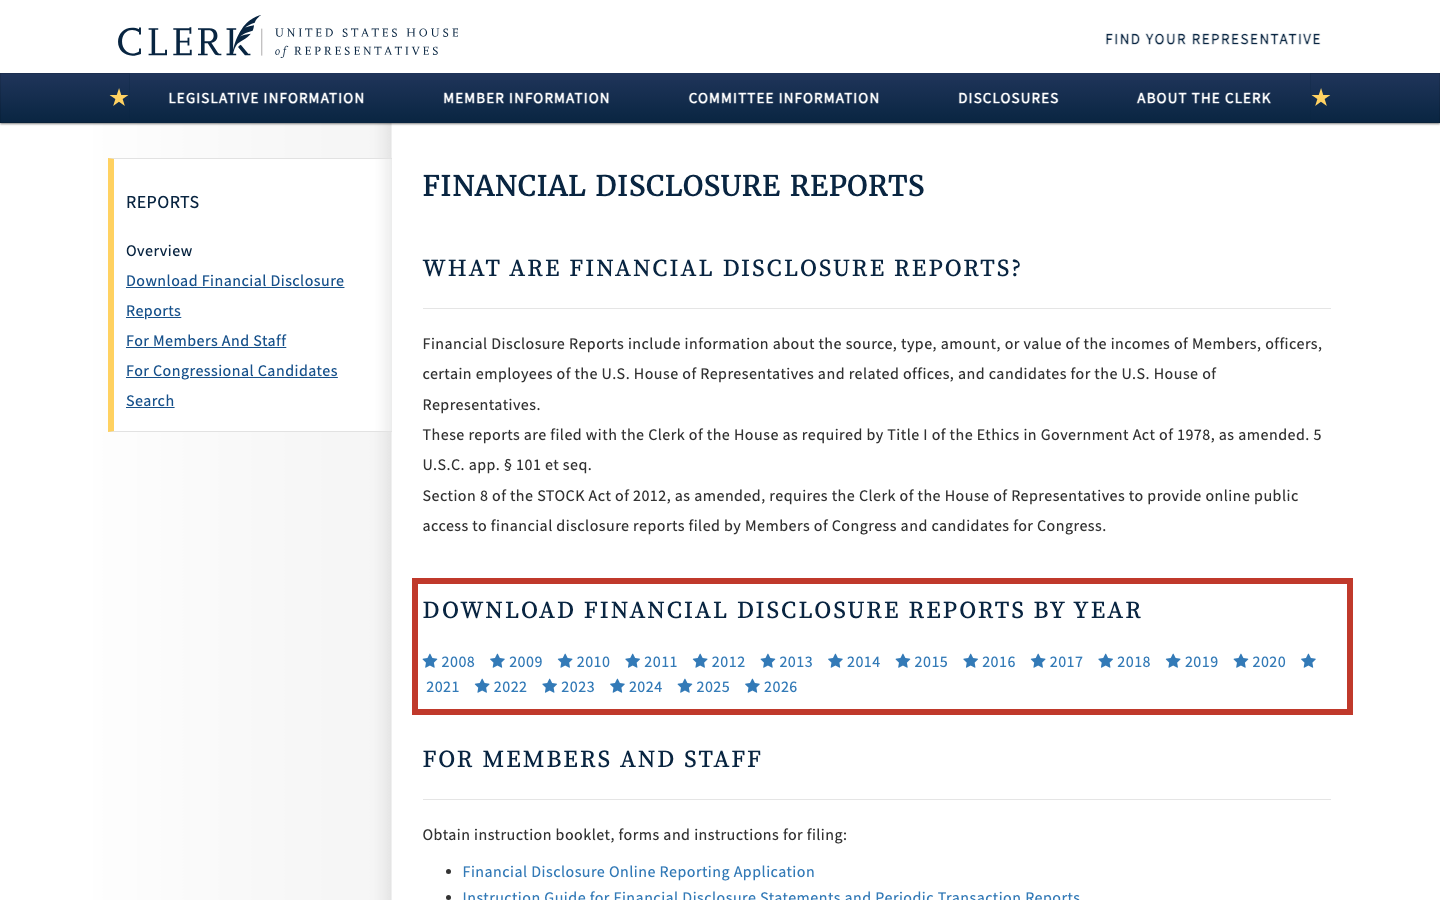
\includegraphics[width=0.97\linewidth]{slides/site_house_clerk.png}}\\[0.8mm]
      {\footnotesize \href{https://disclosures-clerk.house.gov/FinancialDisclosure}%
       {\texttt{disclosures-clerk.house.gov}}} {\scriptsize\color{black!55}(cliquable)}
    \end{column}
    \begin{column}{0.34\textwidth}
      \vspace{6mm}
      {\footnotesize on accède au site public de la Chambre :}\\[3mm]
      · une \textbf{liste de téléchargements}\\[2mm]
      · \textbf{une archive par année} (zone encadrée)\\[2mm]
      · on prend les années \textbf{2014 → 2026}
    \end{column}
  \end{columns}
\end{frame}

% ── C2 · ZIP → index XML ── (URLs house/acquire.py ; un <Member> par dépôt)
\begin{frame}{La Chambre (2/6) — l'archive ZIP contient l'index XML}
  \begin{columns}[T]
    \begin{column}{0.44\textwidth}
      \centering
      \begin{tikzpicture}[node distance=6mm]
        \node[step=helec, text width=4.6cm] (z) {on télécharge l'archive de l'année\\[1mm]\co{2024FD.zip}};
        \node[step=helec, text width=4.6cm, below=of z] (x) {on la dézippe → un fichier\\[1mm]\co{2024FD.xml}};
        \node[step=grisC, text width=4.6cm, below=of x] (i) {c'est l'\textbf{index annuel} :\\un bloc \co{<Member>} par \textbf{dépôt}};
        \draw[arr] (z) -- (x); \draw[arr] (x) -- (i);
      \end{tikzpicture}\\[2mm]
      {\scriptsize\color{black!55} \href{https://disclosures-clerk.house.gov/public_disc/financial-pdfs/2024FD.zip}%
       {\texttt{…/financial-pdfs/2024FD.zip}}}
    \end{column}
    \begin{column}{0.54\textwidth}\centering
      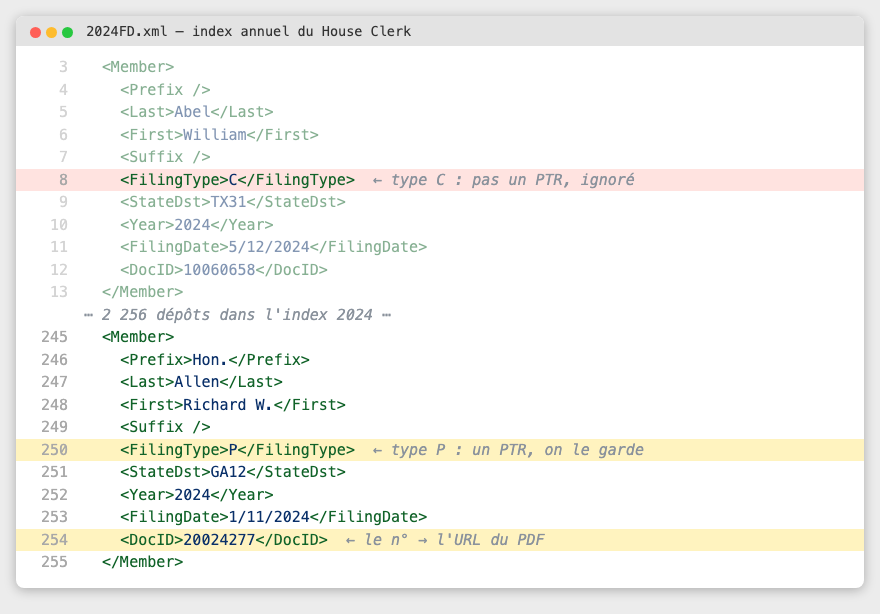
\includegraphics[width=\linewidth]{slides/fichier_index_xml.png}
    \end{column}
  \end{columns}
\end{frame}

% ── C3 · FilingType = P ── (répartition réelle 35 315 dépôts ; fig_filingtypes)
\begin{frame}{La Chambre (3/6) — on ne garde que les PTR (\texttt{FilingType = P})}
  \centering
  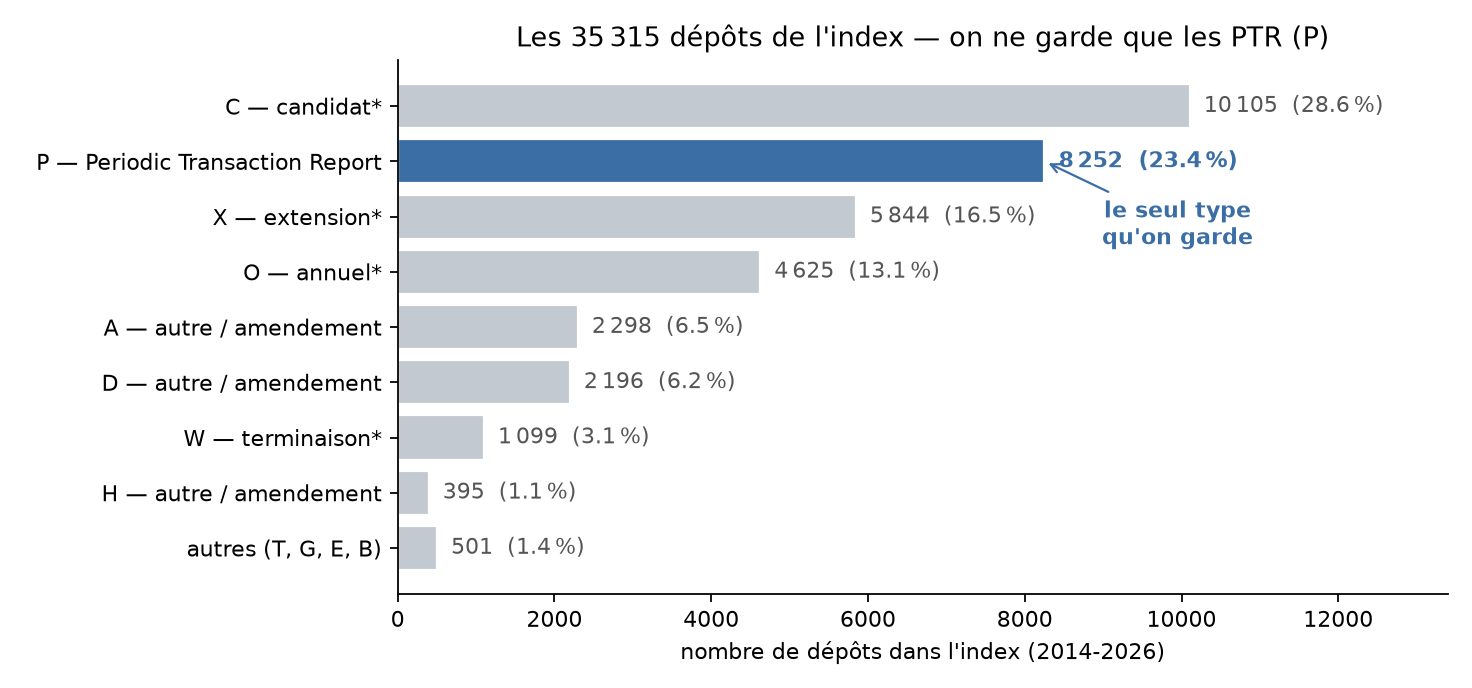
\includegraphics[width=0.76\textwidth]{slides/fig_filingtypes.png}\\[1.5mm]
  {\footnotesize \textbf{P} = \emph{Periodic Transaction Report} — les \textbf{déclarations de
   transactions boursières}, la seule chose qui nous intéresse.}\\[0.8mm]
  {\scriptsize\color{black!60} les autres = candidatures, rapports annuels, demandes de délai,
   notices de campagne, amendements, terminaisons… — pas des transactions
   \;(significations vérifiées en ouvrant les documents)}
\end{frame}

% ═════ Aparté « Les autres dépôts » (5 slides ; les 5 fiches par type sont en annexe) ═════
% chiffres : docs/ANALYSE_FILING_TYPES_HOUSE.md

% ── AD0 · Récap visuel : le cycle de vie ── (schéma fig_cycle_vie, profil mesuré)
\begin{frame}{Les autres dépôts (1/5) — le cycle de vie d'un élu}
  \centering
  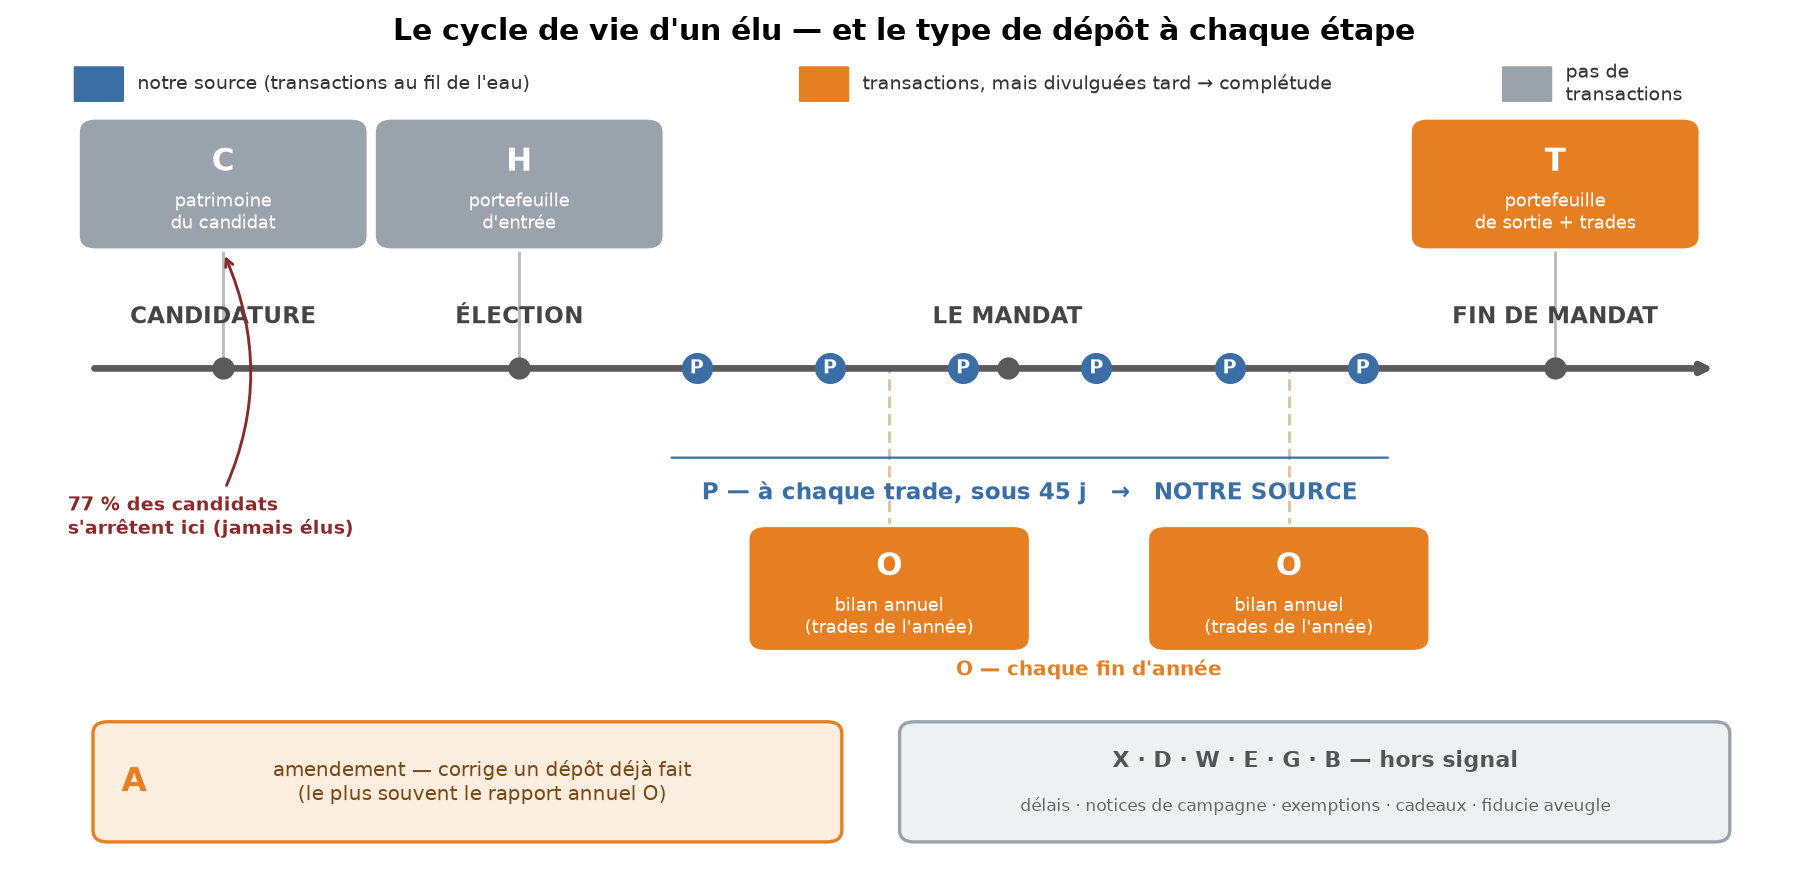
\includegraphics[width=0.84\textwidth]{slides/fig_cycle_vie.png}\\[1mm]
  {\scriptsize\color{black!60} chaque étape de la carrière a son type de dépôt —
   seul \textbf{P} (au fil de l'eau) alimente le signal ; \textbf{O/T/A} contiennent
   des transactions mais divulguées trop tard}
\end{frame}

% ── AD0b · Matrice des sections A→J ── (membership vérifié : O/T=ABCDEFGHI, C/H=ACDEFJ)
\begin{frame}{Les autres dépôts (2/5) — le même formulaire, des sections en commun}
  \centering
  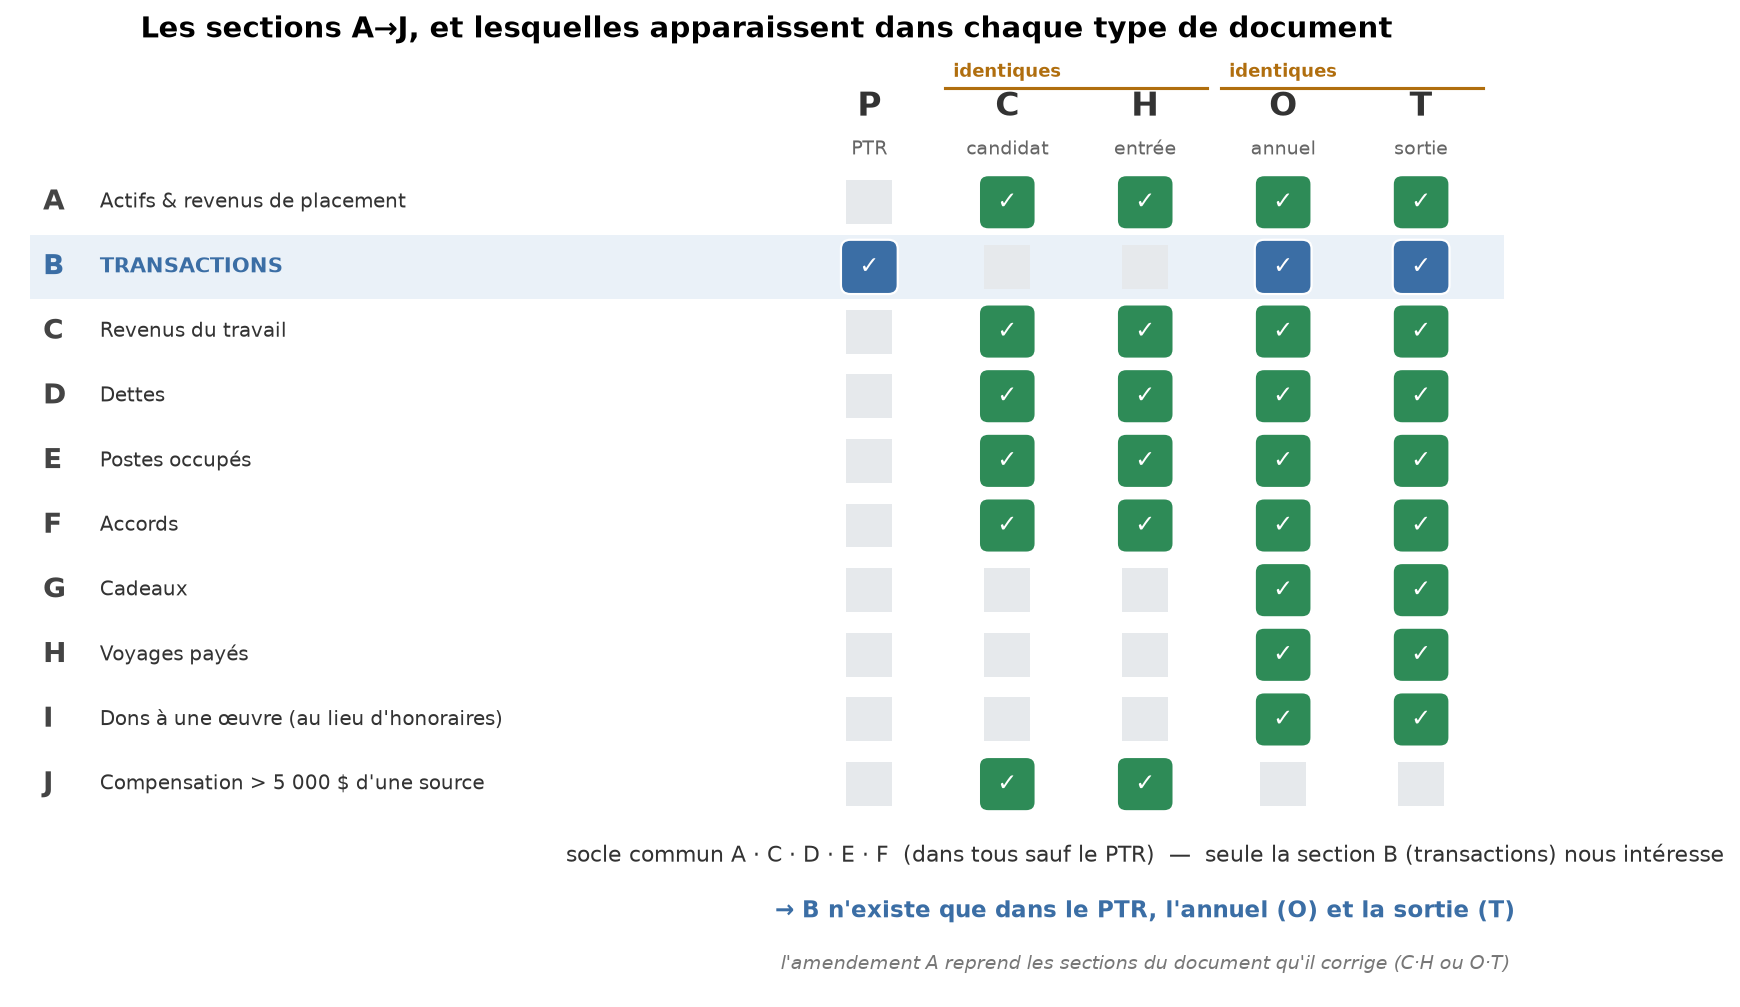
\includegraphics[height=0.60\textheight]{slides/fig_sections_matrix.png}\\[1.5mm]
  {\scriptsize\color{black!60} tous ces documents partagent un socle
   (A·C·D·E·F) — ce qui change, c'est surtout la présence de la
   \textbf{section B, les transactions} ; on trade \textbf{B} (transactions datées),
   \textbf{A} (le patrimoine détenu) sert à \emph{vérifier} qu'on n'a rien loupé}
\end{frame}

% ── AD1 · La famille patrimoine ── (vignettes cliquables ; profil mesuré sur 5 815 docs)
\begin{frame}{Les autres dépôts (3/5) — la famille « patrimoine »}
  \centering
  {\footnotesize cinq types, un socle commun (le \emph{Financial Disclosure Report}) —
   mais les \textbf{transactions (Schedule B) n'existent que dans O, T et leurs
   amendements}}\\[2mm]
  \begin{columns}[T]
    \begin{column}{0.19\textwidth}\centering
      \href{https://disclosures-clerk.house.gov/public_disc/financial-pdfs/2023/10059952.pdf}{\fcolorbox{black!30}{white}{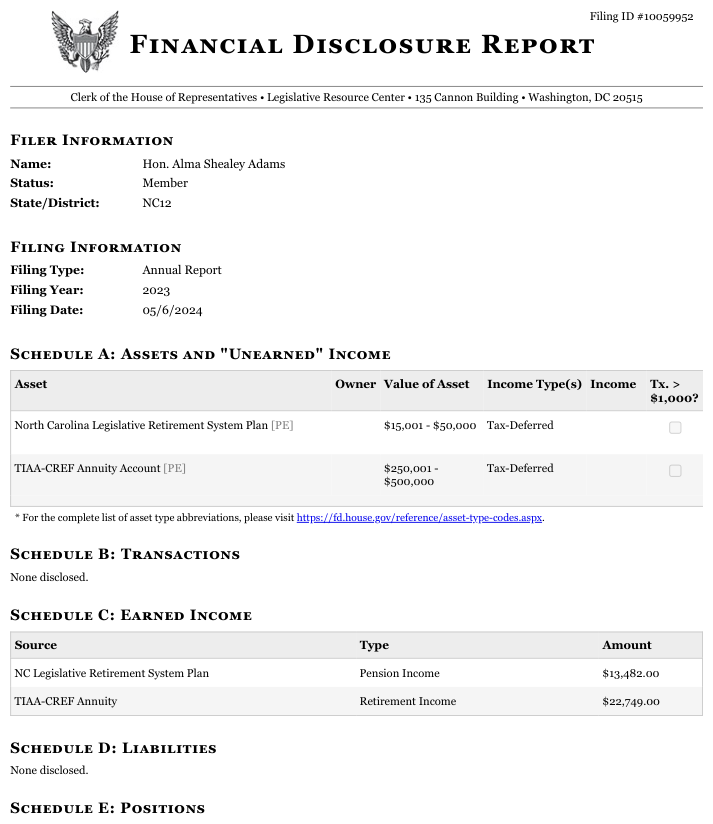
\includegraphics[height=31mm]{slides/ftype_o.png}}}\\[0.8mm]
      {\footnotesize\textbf{O — Annual}}\\{\scriptsize bilan annuel d'un membre}
    \end{column}
    \begin{column}{0.19\textwidth}\centering
      \href{https://disclosures-clerk.house.gov/public_disc/financial-pdfs/2023/10056211.pdf}{\fcolorbox{black!30}{white}{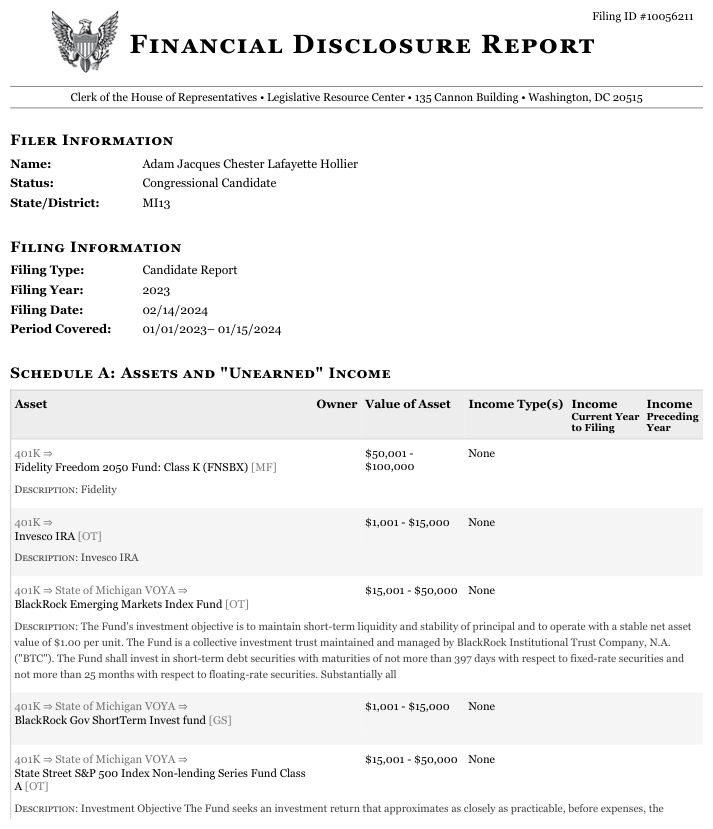
\includegraphics[height=31mm]{slides/ftype_c.png}}}\\[0.8mm]
      {\footnotesize\textbf{C — Candidate}}\\{\scriptsize candidat au Congrès}
    \end{column}
    \begin{column}{0.19\textwidth}\centering
      \href{https://disclosures-clerk.house.gov/public_disc/financial-pdfs/2023/10062638.pdf}{\fcolorbox{black!30}{white}{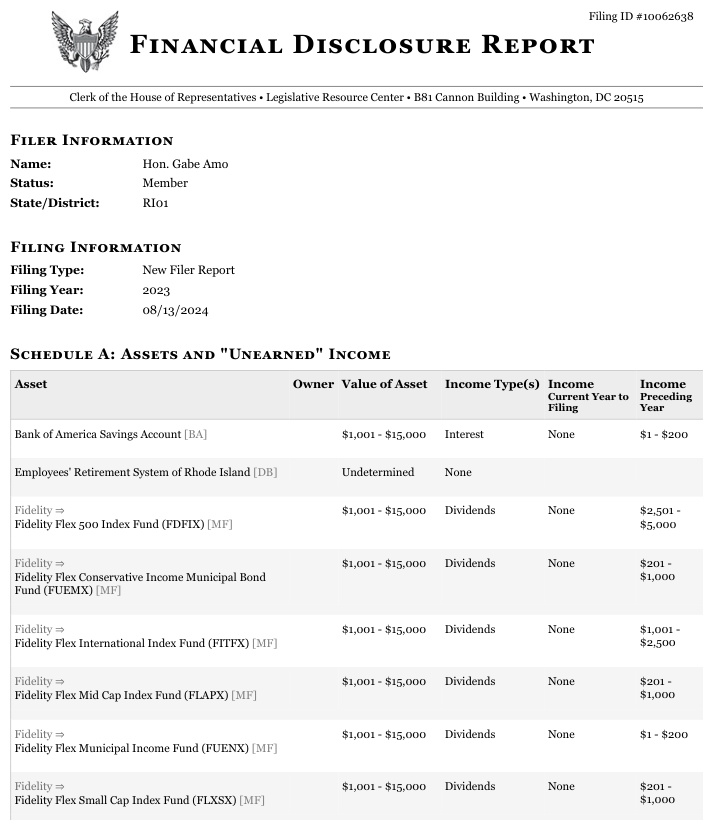
\includegraphics[height=31mm]{slides/ftype_h.png}}}\\[0.8mm]
      {\footnotesize\textbf{H — New Filer}}\\{\scriptsize première déclaration}
    \end{column}
    \begin{column}{0.19\textwidth}\centering
      \href{https://disclosures-clerk.house.gov/public_disc/financial-pdfs/2023/10050798.pdf}{\fcolorbox{black!30}{white}{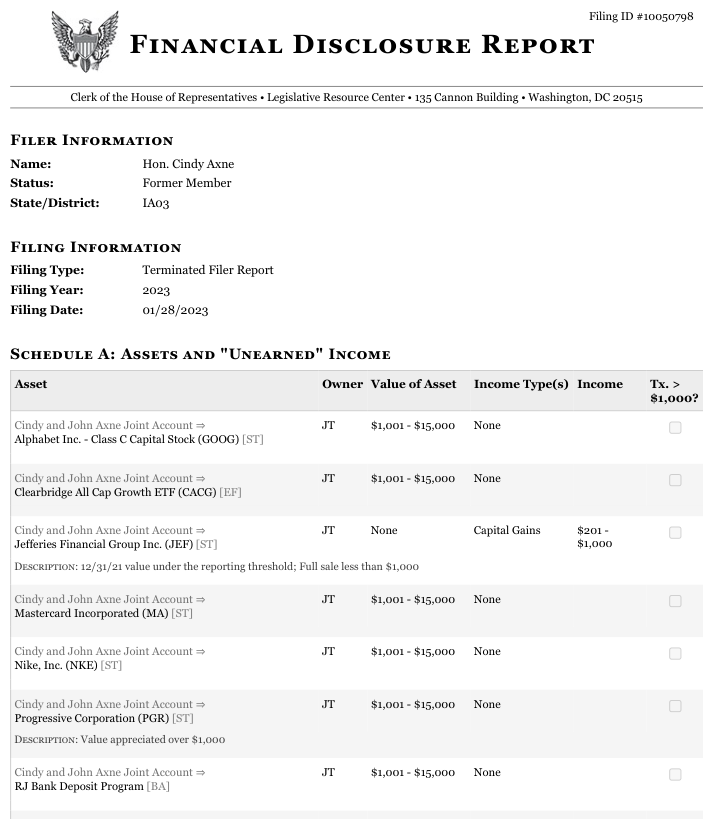
\includegraphics[height=31mm]{slides/ftype_t.png}}}\\[0.8mm]
      {\footnotesize\textbf{T — Termination}}\\{\scriptsize déclaration de départ}
    \end{column}
    \begin{column}{0.19\textwidth}\centering
      \href{https://disclosures-clerk.house.gov/public_disc/financial-pdfs/2023/10062190.pdf}{\fcolorbox{black!30}{white}{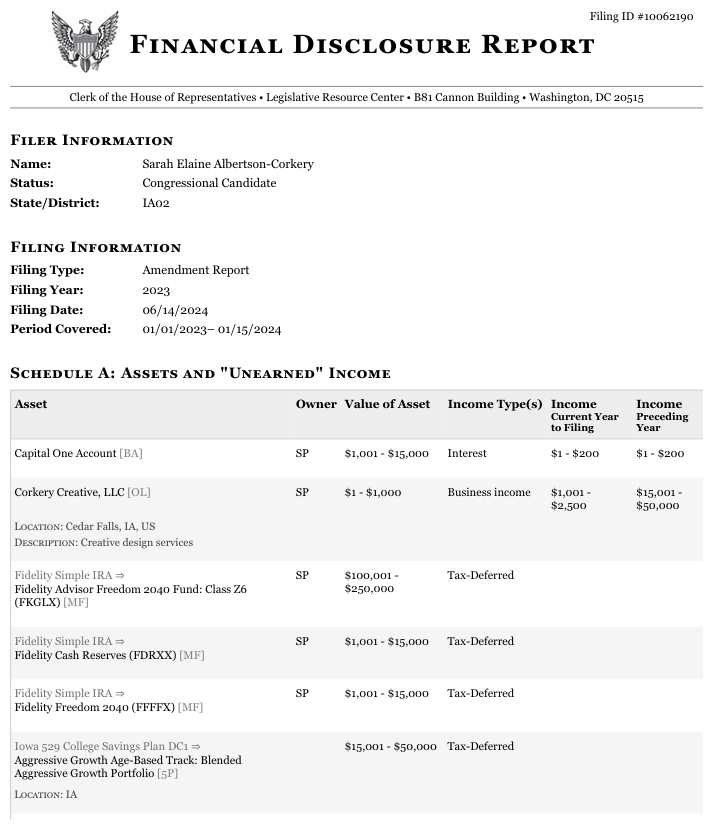
\includegraphics[height=31mm]{slides/ftype_a.png}}}\\[0.8mm]
      {\footnotesize\textbf{A — Amendment}}\\{\scriptsize correction d'un dépôt}
    \end{column}
  \end{columns}
  \vspace{2.5mm}
  \badge{helec}{chaque vignette est cliquable → ouvre le vrai document}\quad
  {\scriptsize\color{black!60} fiche détaillée de chacun des cinq types : \textbf{en annexe}}
\end{frame}

% ── AD2 · Il y a des transactions dedans ── (Pelosi annuel 2015, Schedule B p.6)
\begin{frame}{Les autres dépôts (4/5) — surprise : il y a des transactions dedans}
  \centering
  \badge{warnorange}{type O — Annual Report 2015, Nancy Pelosi}\\[2mm]
  \fcolorbox{black!25}{white}{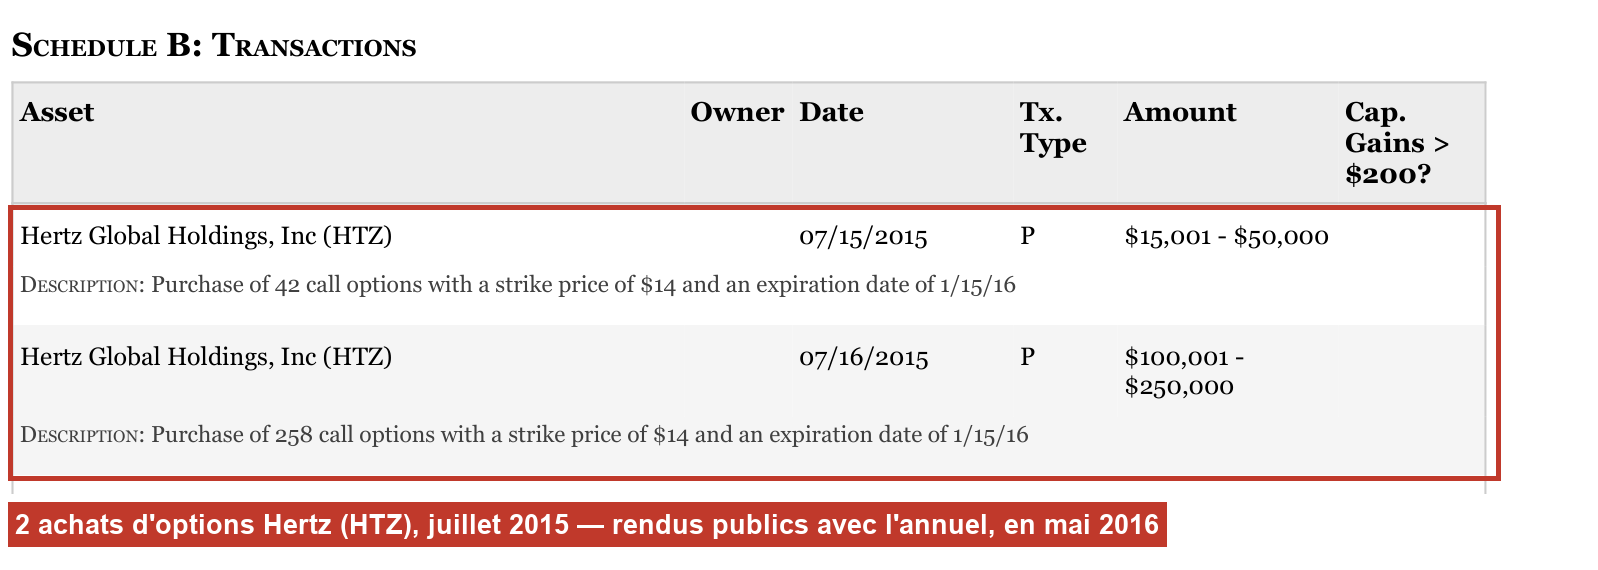
\includegraphics[width=0.86\textwidth]{slides/fig_pelosi_schedb.png}}\\[1.5mm]
  {\footnotesize la \textbf{Schedule B} d'un rapport annuel \textbf{récapitule les
   trades de l'année}. Ceux de Pelosi sont tous \textbf{déjà dans nos PTR} (vérifié,
   delta 0 jour) — mais est-ce le cas de tout le monde ? La réponse, mesurée sur
   \textbf{tout} le corpus, est dans la partie « \textbf{la refonte V1} ». \quad
   {\scriptsize\color{black!60}
   \href{https://disclosures-clerk.house.gov/public_disc/financial-pdfs/2015/10010857.pdf}{ouvrir ce rapport (cliquable)}}}
\end{frame}

% ── AD3 · Les administratifs + blind trust ── (vignettes réelles)
\begin{frame}{Les autres dépôts (5/5) — les administratifs, et le cas à part}
  \centering
  {\footnotesize cinq types \textbf{sans aucune transaction} :}\\[1.5mm]
  \begin{columns}[T]
    \begin{column}{0.19\textwidth}\centering
      \fcolorbox{black!30}{white}{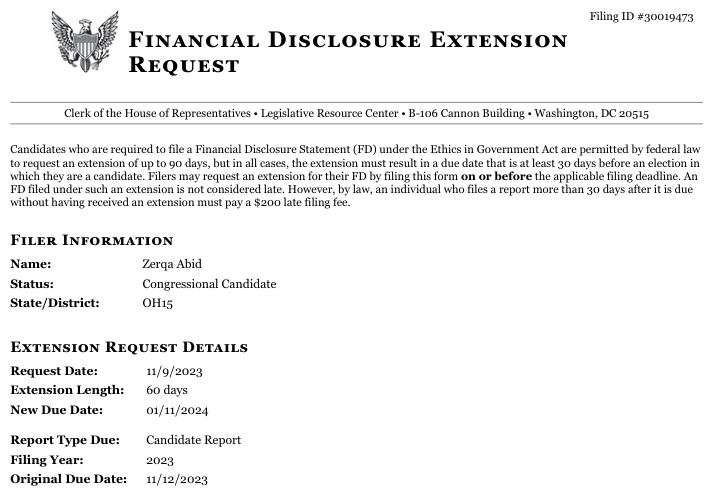
\includegraphics[height=24mm]{slides/ftype_x.png}}\\[0.6mm]
      {\scriptsize\textbf{X — Extension}\\demande de délai}
    \end{column}
    \begin{column}{0.19\textwidth}\centering
      \fcolorbox{black!30}{white}{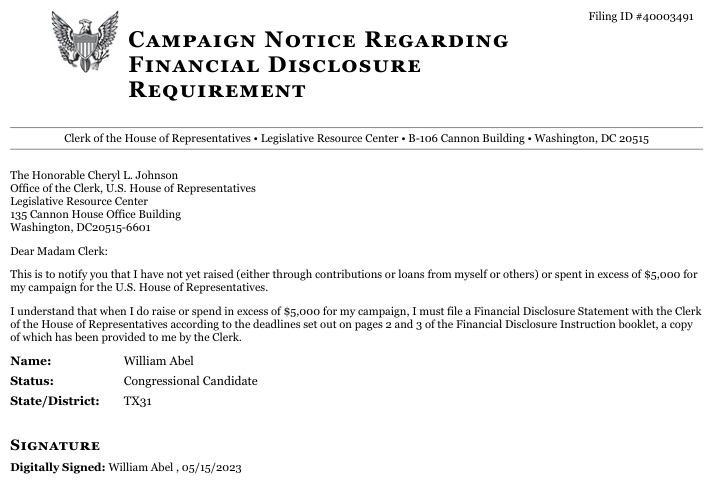
\includegraphics[height=24mm]{slides/ftype_d.png}}\\[0.6mm]
      {\scriptsize\textbf{D — Campaign Notice}\\« < 5\,000 \$ levés »}
    \end{column}
    \begin{column}{0.19\textwidth}\centering
      \fcolorbox{black!30}{white}{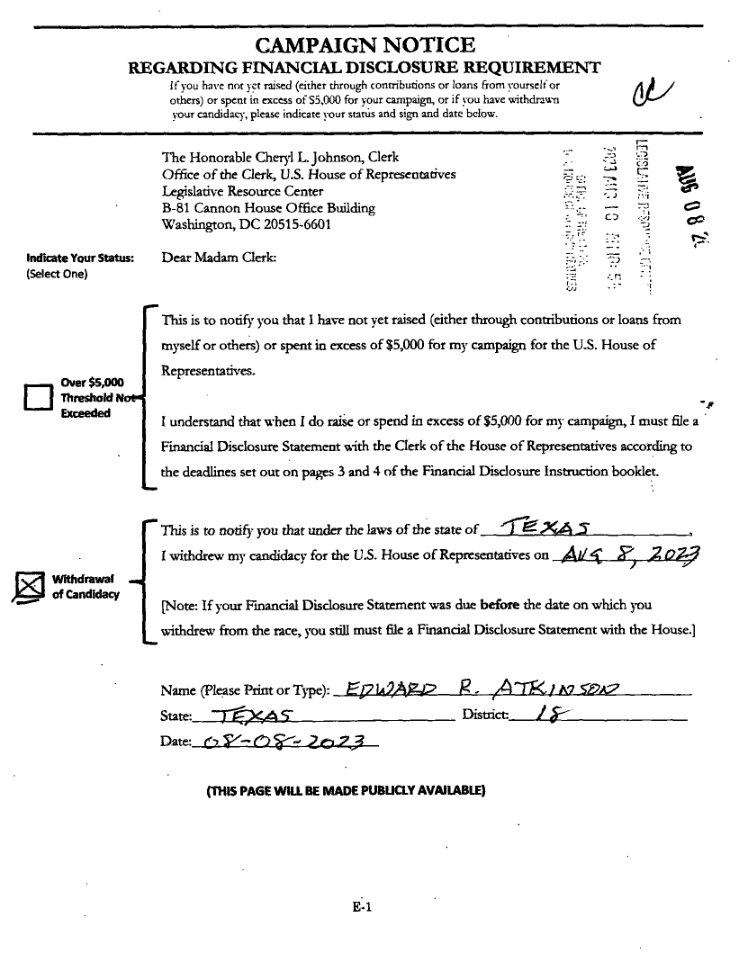
\includegraphics[height=24mm]{slides/ftype_w.png}}\\[0.6mm]
      {\scriptsize\textbf{W — idem, papier}\\(ou retrait)}
    \end{column}
    \begin{column}{0.19\textwidth}\centering
      \fcolorbox{black!30}{white}{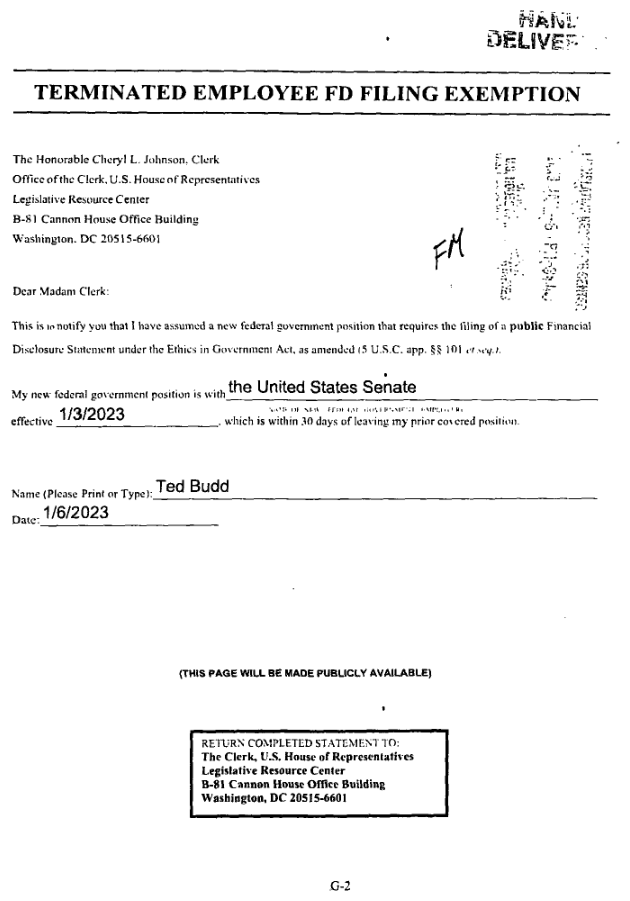
\includegraphics[height=24mm]{slides/ftype_e.png}}\\[0.6mm]
      {\scriptsize\textbf{E — Exemption}\\départ vers un poste fédéral}
    \end{column}
    \begin{column}{0.19\textwidth}\centering
      \fcolorbox{black!30}{white}{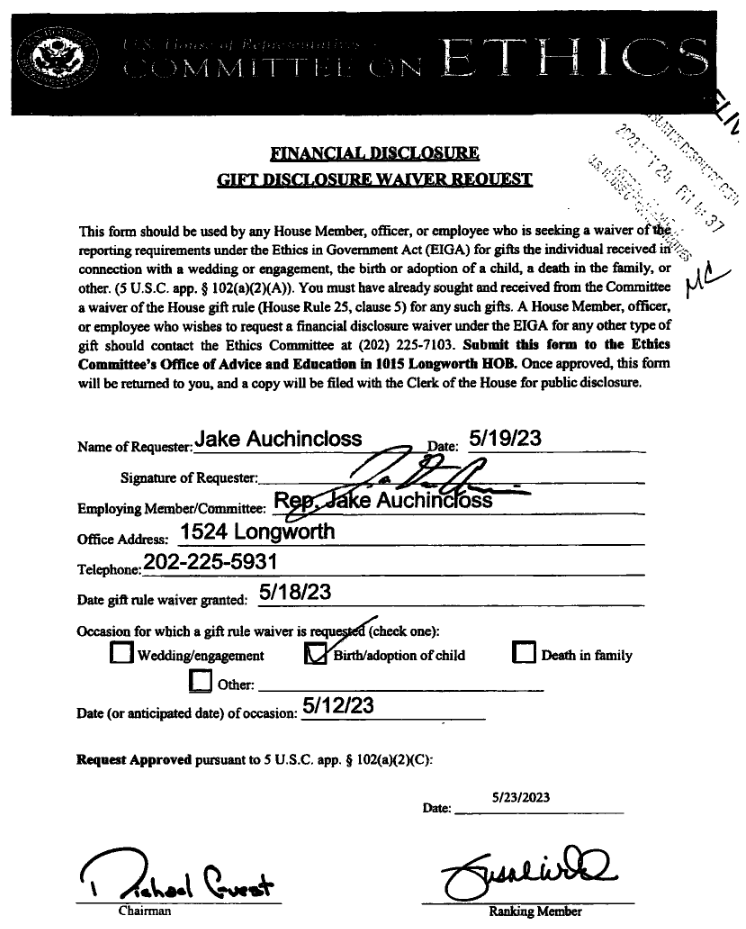
\includegraphics[height=24mm]{slides/ftype_g.png}}\\[0.6mm]
      {\scriptsize\textbf{G — Gift Waiver}\\dérogation cadeau}
    \end{column}
  \end{columns}
  \vspace{2.5mm}
  \begin{columns}[c]
    \begin{column}{0.14\textwidth}\centering
      \fcolorbox{alertred}{white}{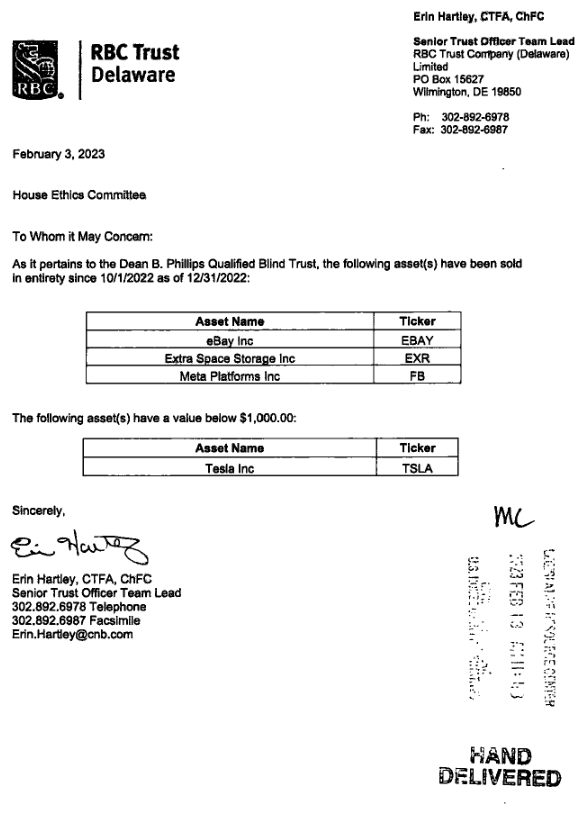
\includegraphics[height=22mm]{slides/ftype_b.png}}
    \end{column}
    \begin{column}{0.80\textwidth}
      \colorbox{alertred!10}{\parbox{0.97\linewidth}{\footnotesize
        \textbf{\textcolor{alertred}{B — Blind Trust}} (23 dépôts) : la banque du
        \emph{trust} liste des ventes (eBay, Meta, Tesla…) — de vraies transactions,
        mais \textbf{pas décidées par l'élu} : c'est le principe de la fiducie aveugle.}}
    \end{column}
  \end{columns}
\end{frame}

% ── C4 · DocID → PDF lisible ou scanné ── (préfixe 2/8/9 ; 71/29 %)
\begin{frame}{La Chambre (4/6) — le \texttt{DocID} ouvre le document (un PDF)}
  \centering
  \vspace{2mm}
  \resizebox{0.96\textwidth}{!}{%
  \begin{tikzpicture}[node distance=9mm]
    \node[step=helec, text width=3.2cm] (d) {le \co{DocID} du dépôt\\[1mm]\co{20024277}};
    \node[step=grisC, text width=4.8cm, right=10mm of d] (u)
      {une URL de PDF\\[1mm]{\scriptsize\ttfamily …/ptr-pdfs/2024/20024277.pdf}};
    \node[step=helec, fill=helec!16, text width=4.4cm, above right=1mm and 11mm of u] (lis)
      {\textbf{PDF lisible} (numérique)\\{\scriptsize couche texte — DocID en \co{2…}}};
    \node[step=hocr, fill=hocr!40, text width=4.4cm, below right=1mm and 11mm of u] (sc)
      {\textbf{PDF scanné} (image)\\{\scriptsize à lire par OCR — DocID en \co{8…}/\co{9…}}};
    \draw[arr] (d) -- (u);
    \draw[arr] (u.east) -- (lis.west);
    \draw[arr] (u.east) -- (sc.west);
  \end{tikzpicture}}

  \vspace{5mm}
  {\footnotesize selon le dépôt, le PDF est déjà \textbf{lisible par machine}
   ou seulement une \textbf{image scannée} — ce sont les deux voies suivantes.}\\[1mm]
  {\scriptsize\color{black!60} sur les PTR : environ \textbf{71 \%} lisibles · \textbf{29 \%} scannés}
\end{frame}

% ── C5 · PTR lisible (exemple) ── (RAPPORT_FINAL §4.3 « dans la source »)
\begin{frame}{La Chambre (5/6) — le document : un PTR lisible}
  \begin{columns}[T]
    \begin{column}{0.55\textwidth}\centering
      \fcolorbox{helec}{white}{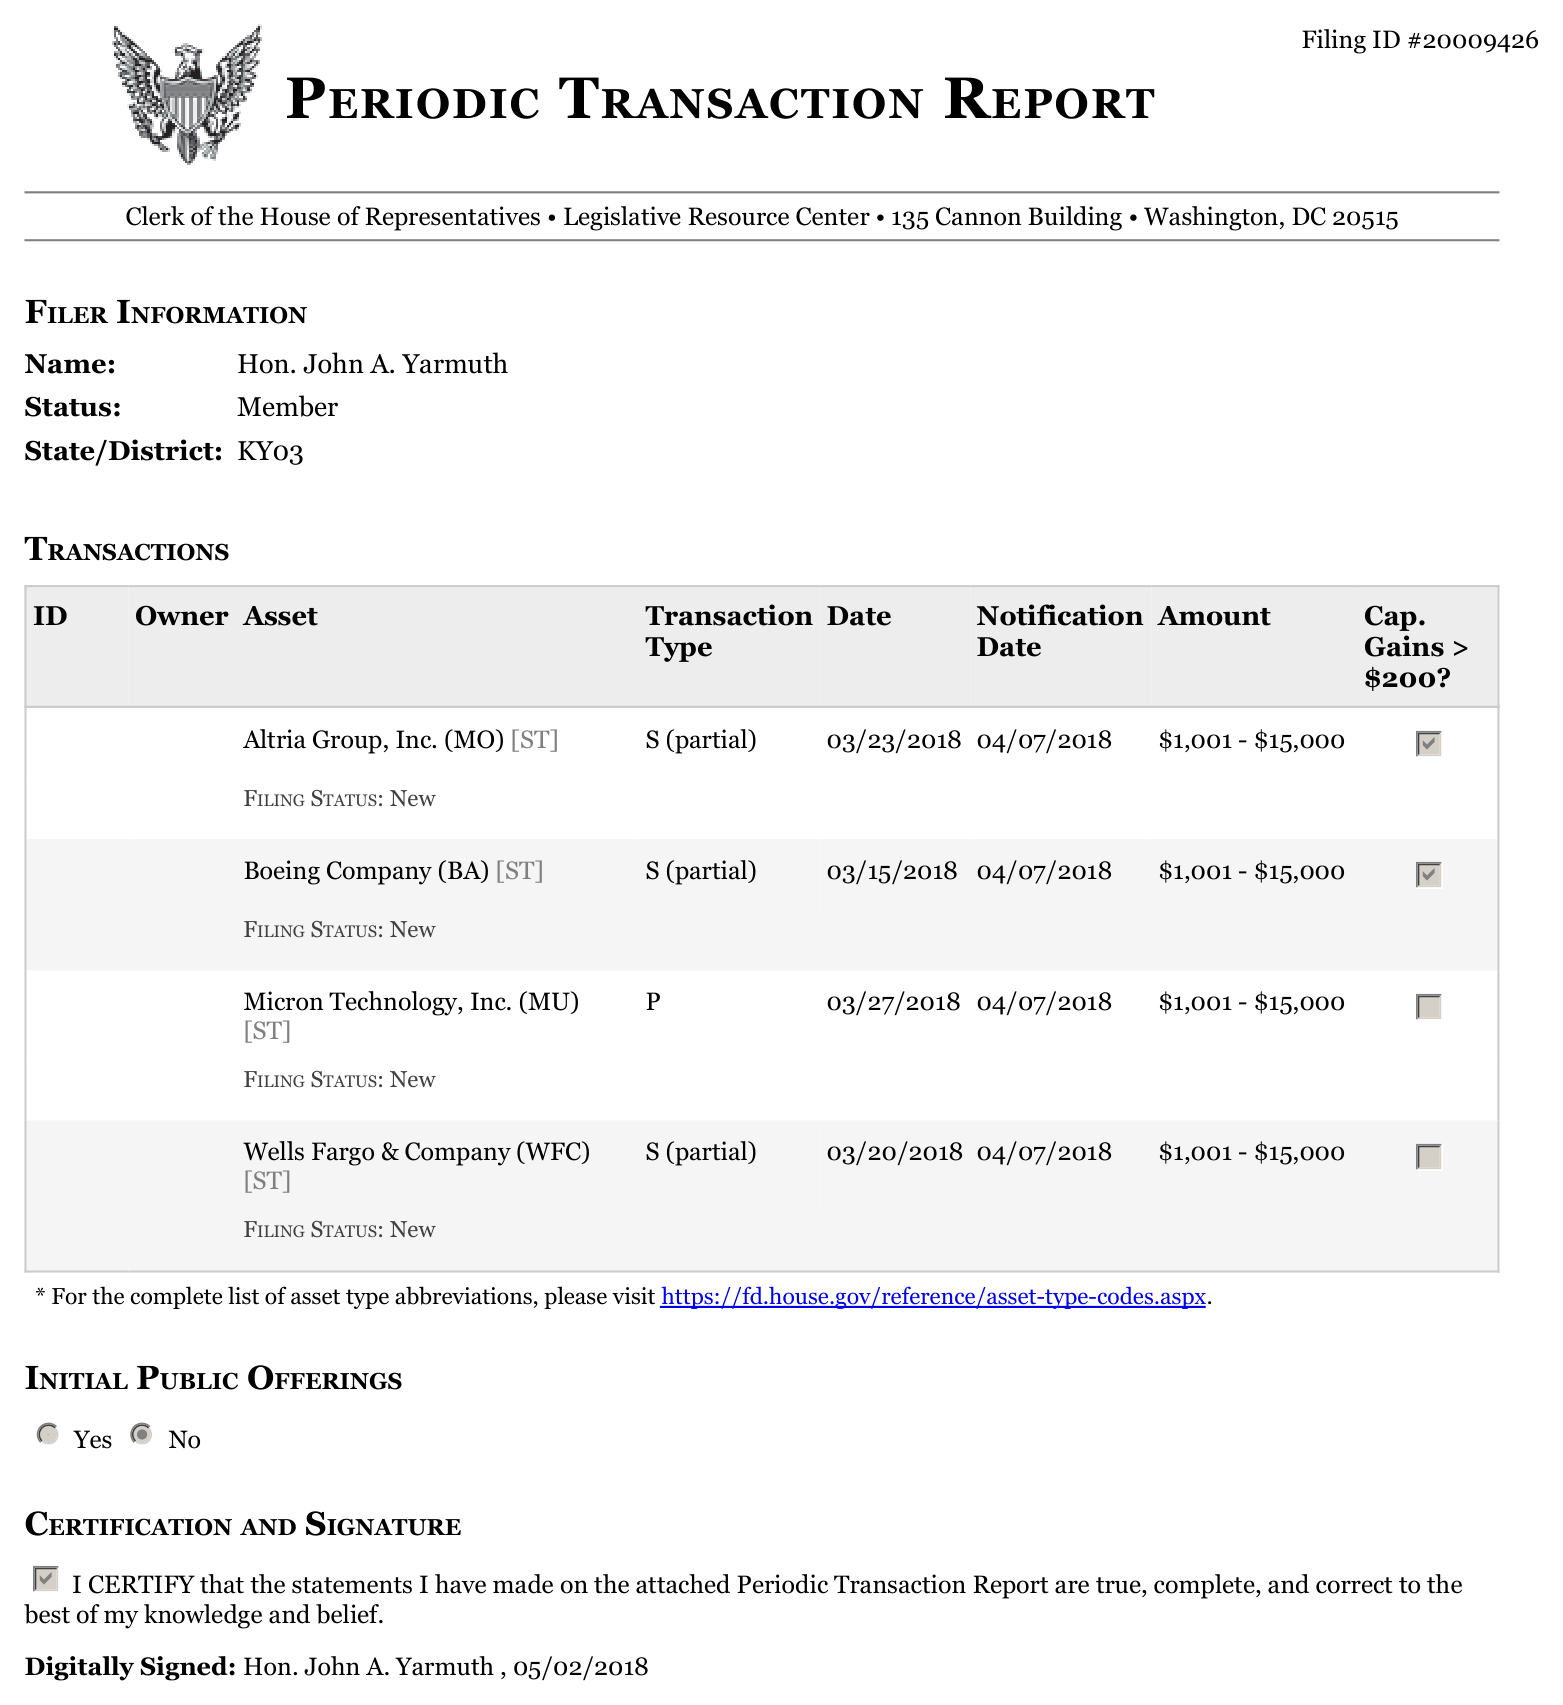
\includegraphics[height=66mm]{slides/fig_ptr_digital.png}}\\[0.5mm]
      {\scriptsize\color{black!60} PTR électronique complet (Hon. John A. Yarmuth, KY03)}
    \end{column}
    \begin{column}{0.43\textwidth}
      \badge{helec}{DocID en \co{2…} → PDF lisible}\\[3mm]
      {\footnotesize
      · un PDF \textbf{avec couche texte} : lisible machine\\[1.5mm]
      · le ticker est imprimé \textbf{entre parenthèses} : \co{(BA)},
        le type d'actif entre crochets : \co{[ST]}\\[1.5mm]
      · deux dates par ligne (trade / notification) + fourchette de montant\\[1.5mm]
      · lisible… mais pas si régulier : \textcolor{alertred}{le défi} sur la slide
        suivante}
    \end{column}
  \end{columns}
\end{frame}

% ── II.3bis · Le défi de l'extraction électronique ── (§4.3 ; audit §4 : 7 996 montants tronqués)
\begin{frame}{La Chambre (5/6) — le défi : lire un PDF irrégulier}
  \begin{columns}[T]
    \begin{column}{0.62\textwidth}\centering
      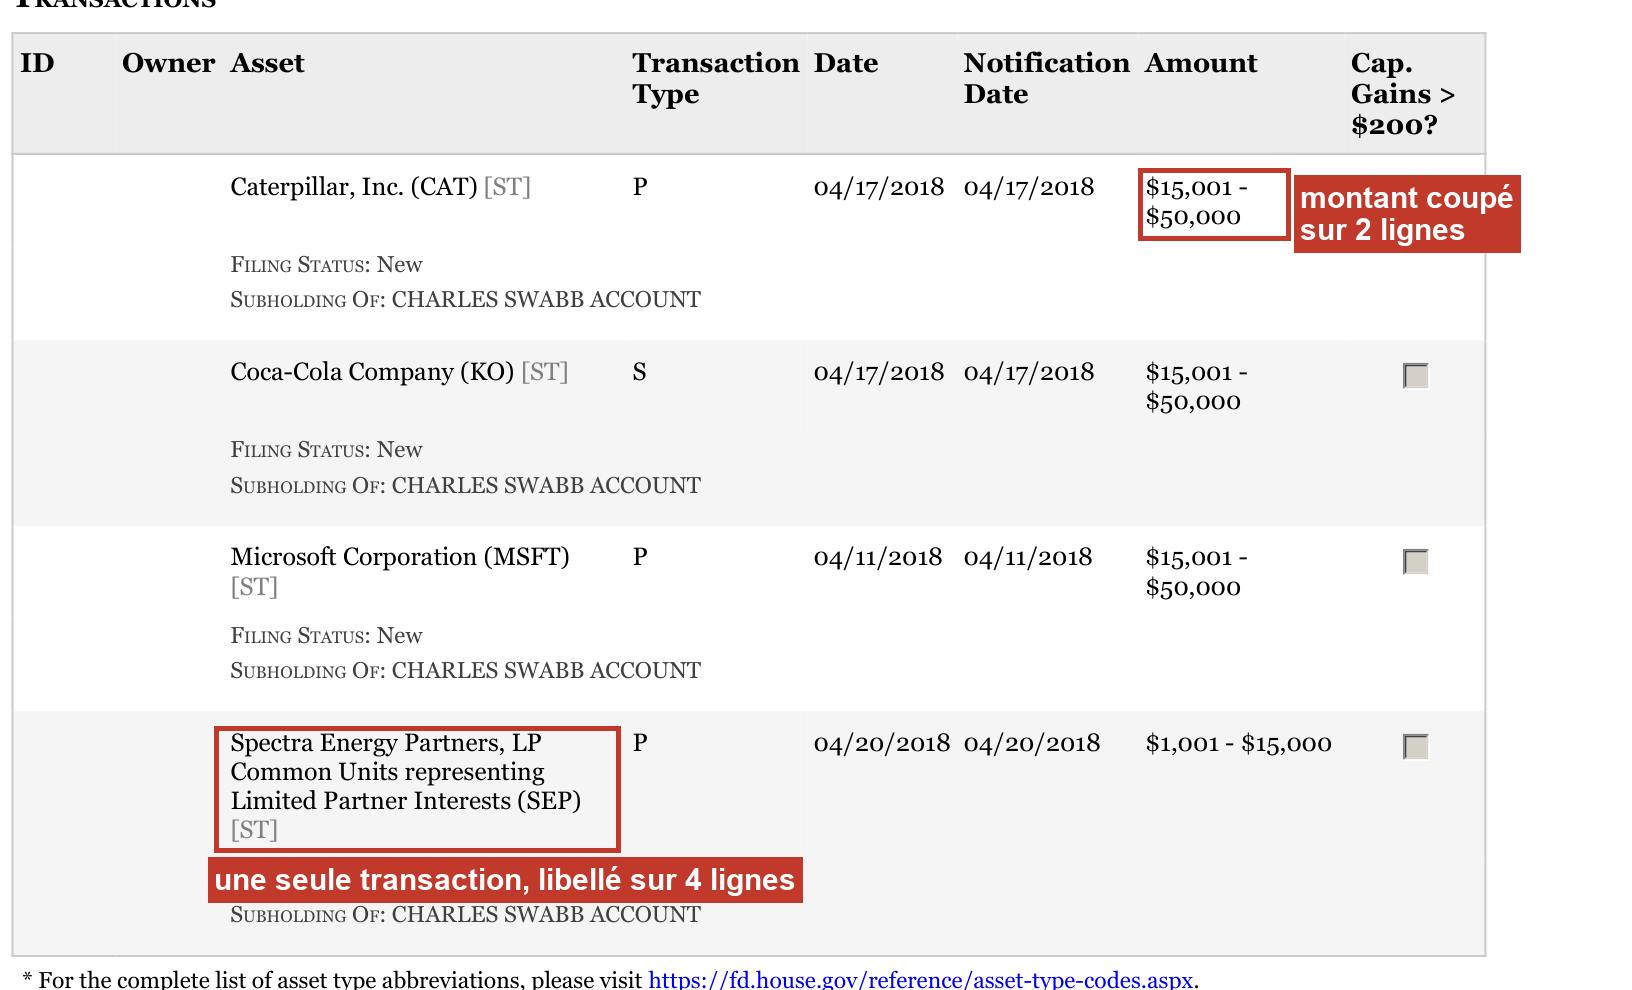
\includegraphics[width=\linewidth]{slides/fig_ptr_multiligne.png}\\[0.5mm]
      {\scriptsize\color{black!60} extrait réel (Hon.\ Bob Gibbs, OH07) — cadres ajoutés}
    \end{column}
    \begin{column}{0.36\textwidth}
      {\footnotesize le PDF n'est \textbf{pas un tableau régulier} :}\\[2mm]
      {\footnotesize
      · le \textbf{montant} déborde sur la ligne suivante
        (\co{\$15,001 -} puis \co{\$50,000})\\[1.5mm]
      · le \textbf{libellé} d'un actif court sur \textbf{4 lignes}\\[1.5mm]
      · un découpage ligne à ligne raterait la moitié}\\[3mm]
      \colorbox{helec}{\parbox{0.95\linewidth}{\footnotesize\color{white}\centering
        → on \textbf{reconstruit} chaque transaction\\
        (recollage des lignes coupées)\\ avant de la lire}}\\[2mm]
      {\scriptsize\color{black!60} le montant coupé à lui seul : \textbf{7\,996}
       lignes réparées}
    \end{column}
  \end{columns}
\end{frame}

% ── II.4 · Chambre scannée : les différents cas (simple, pages entières) ── (§4.5 ; détail à l'étape 5)
\begin{frame}{La Chambre (6/6) — le document : un PTR scanné}
  \centering
  {\footnotesize un scan n'est pas du texte, c'est une \textbf{image} — et il arrive
   sous trois formes (pages réelles) :}\\[2.5mm]
  \begin{columns}[T]
    \begin{column}{0.37\textwidth}\centering
      \fcolorbox{black!30}{white}{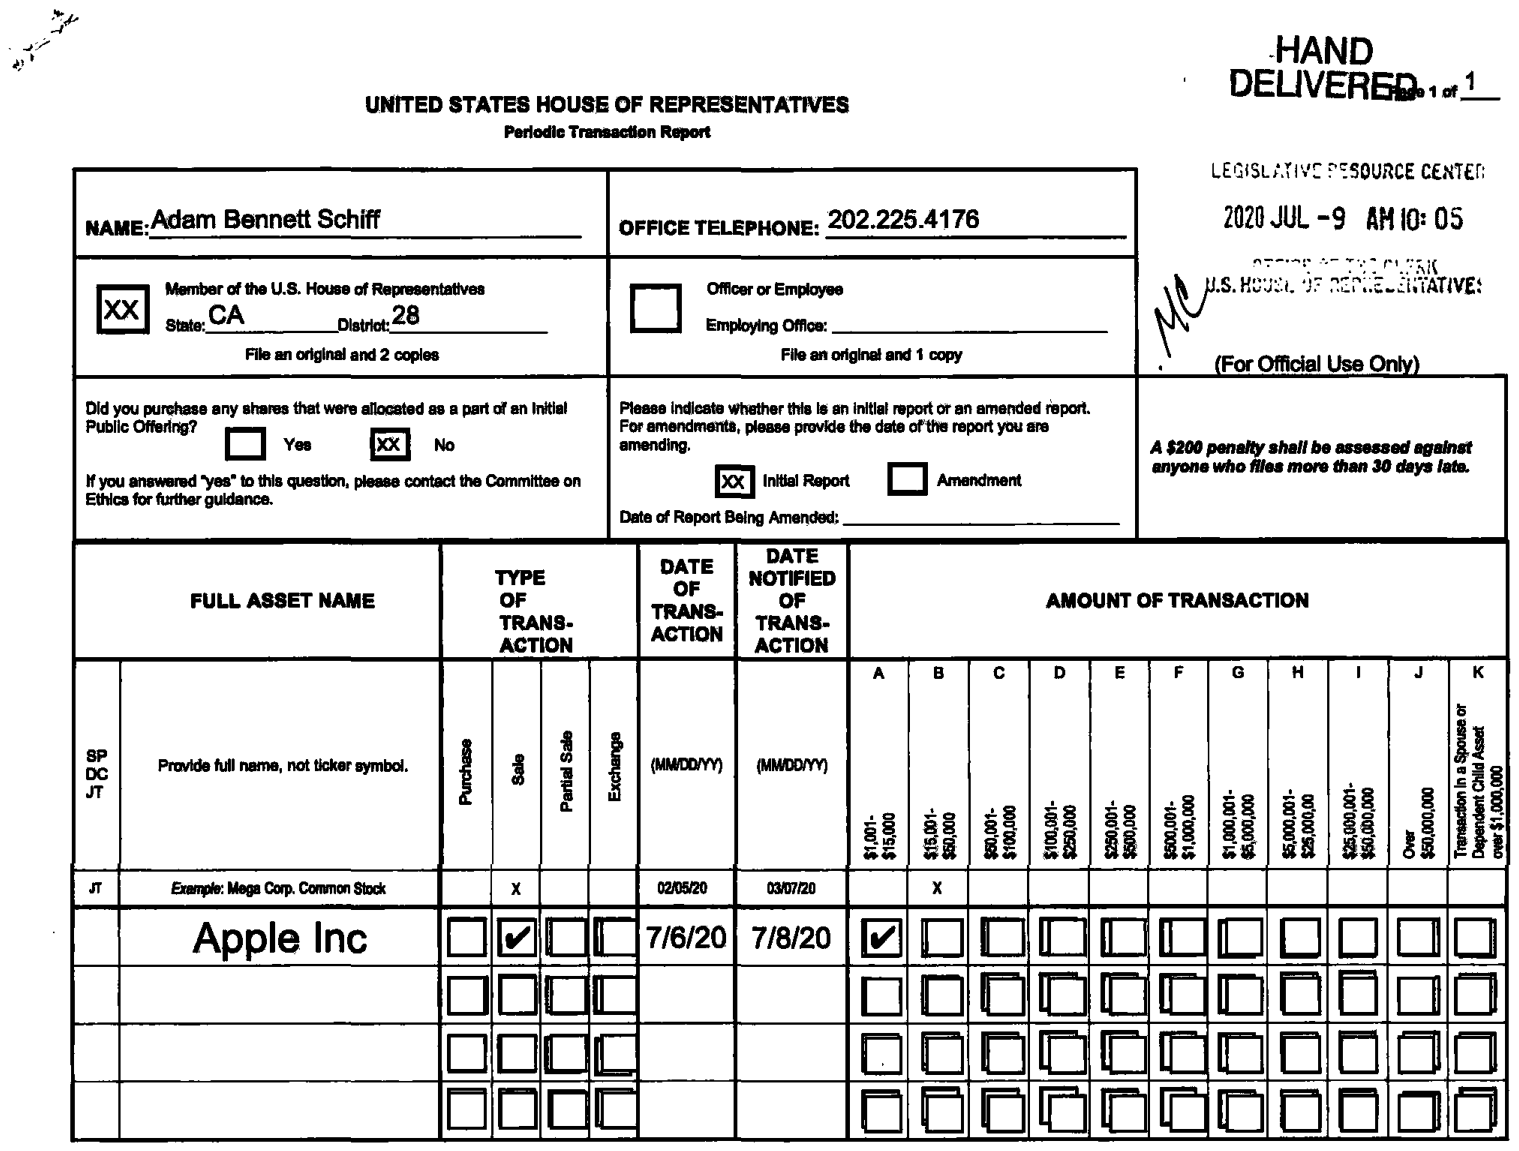
\includegraphics[height=35mm]{slides/scan_full_droit.png}}\\[1.2mm]
      {\footnotesize\textbf{Tapé, droit}}\\[0.3mm]
      {\scriptsize dactylographié, lisible tel quel}
    \end{column}
    \begin{column}{0.21\textwidth}\centering
      \fcolorbox{black!30}{white}{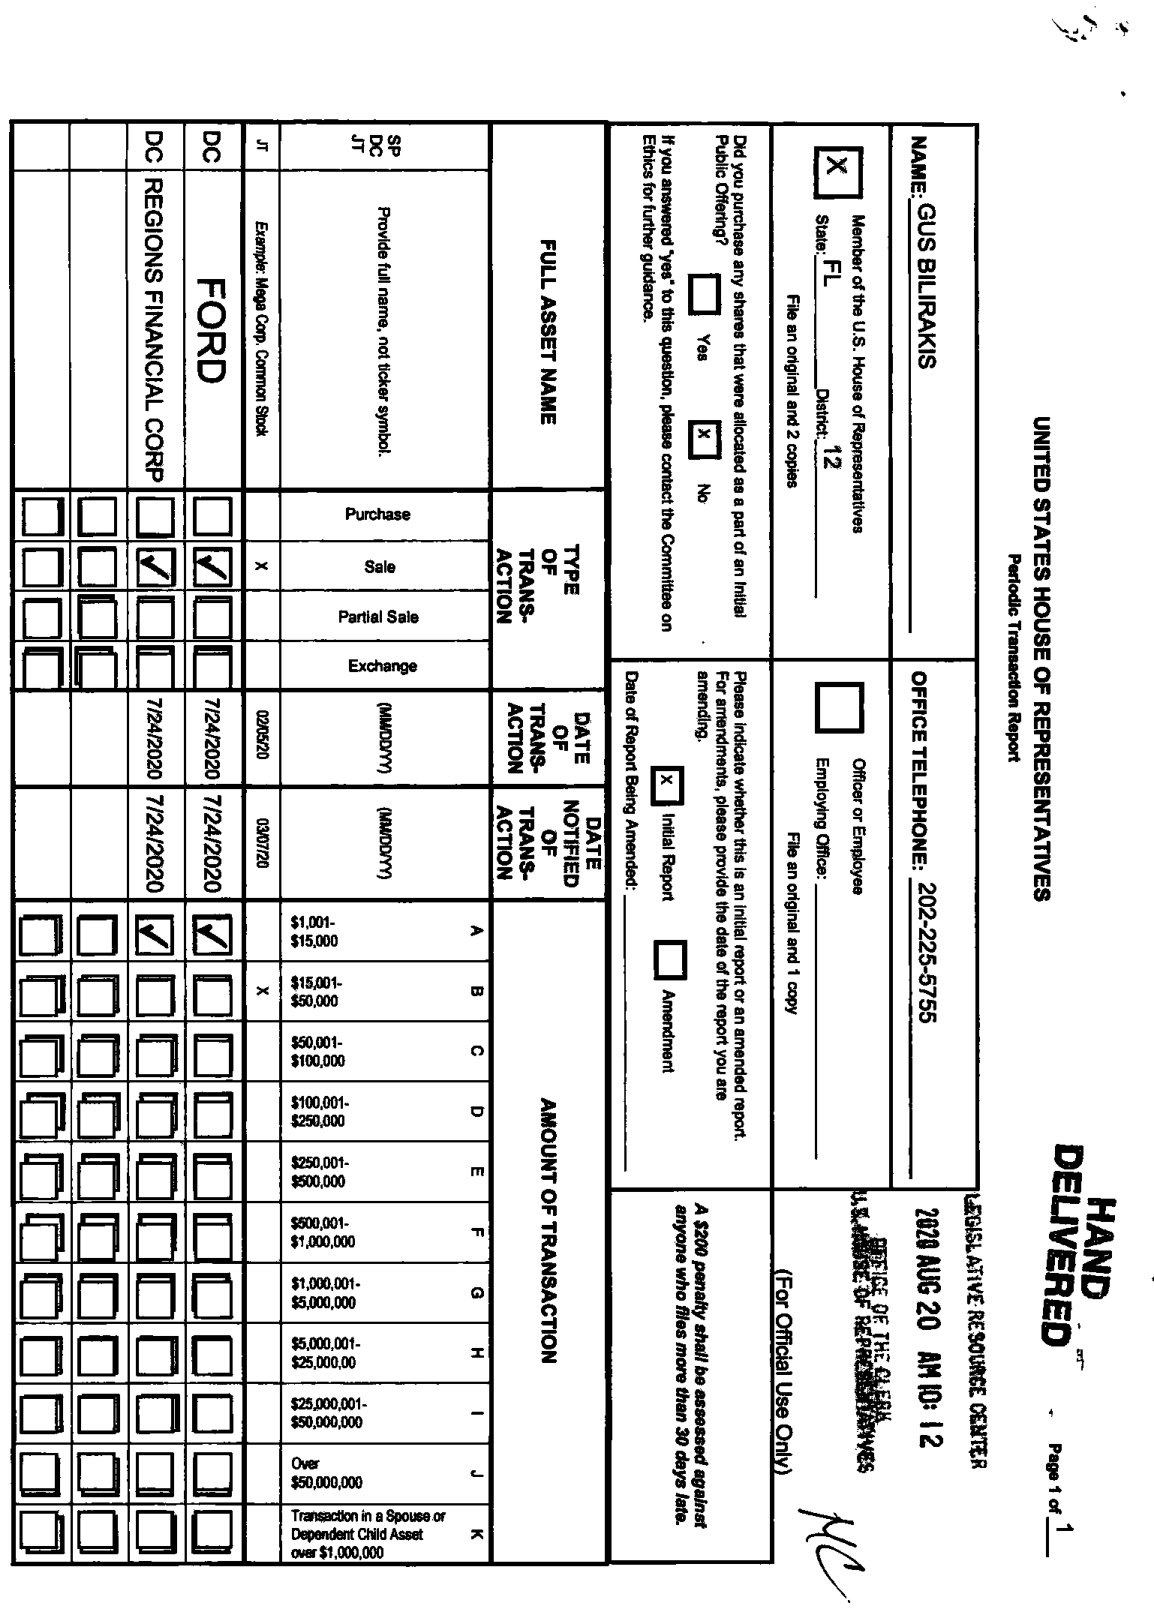
\includegraphics[height=35mm]{slides/scan_full_couche.png}}\\[1.2mm]
      {\footnotesize\textbf{Tapé, couché}}\\[0.3mm]
      {\scriptsize tapé mais \textbf{tourné à 90°}\\(le plus courant)}
    \end{column}
    \begin{column}{0.37\textwidth}\centering
      \fcolorbox{black!30}{white}{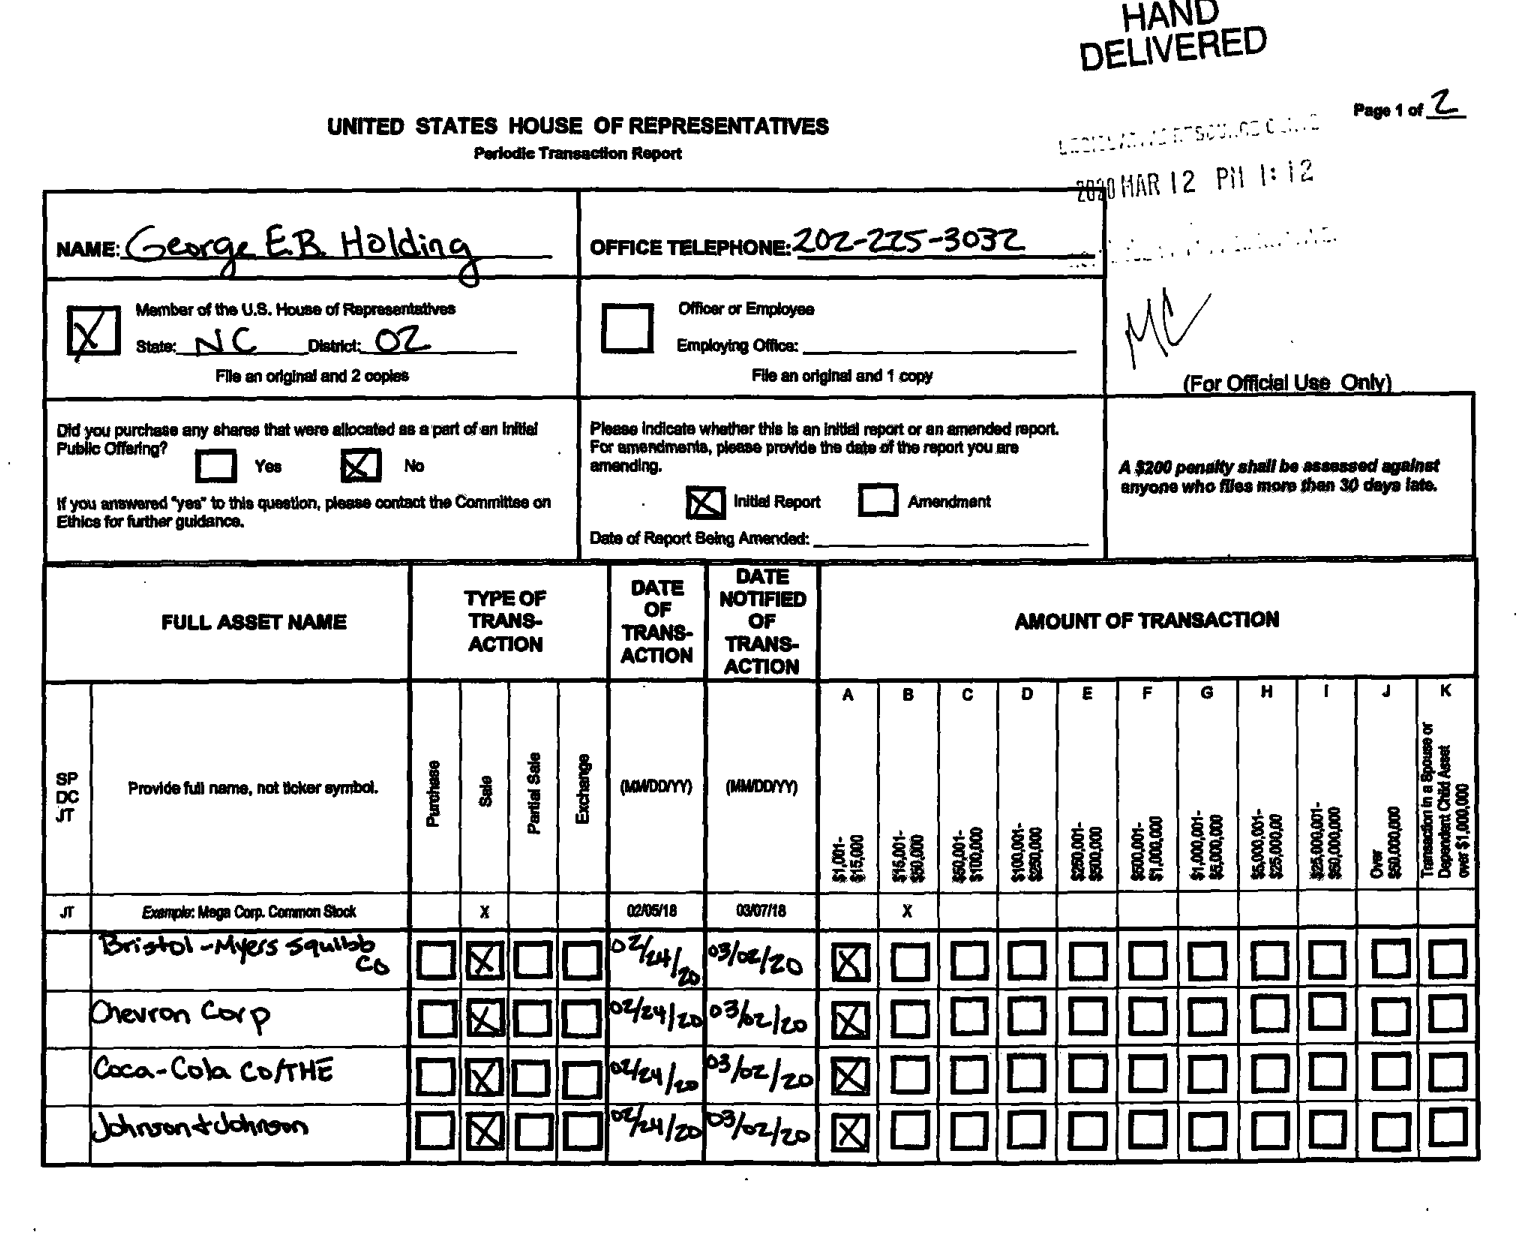
\includegraphics[height=35mm]{slides/scan_full_manuscrit.png}}\\[1.2mm]
      {\footnotesize\textbf{Manuscrit}}\\[0.3mm]
      {\scriptsize rempli \textbf{à la main}, en cursif}
    \end{column}
  \end{columns}
  \vspace{2mm}
  \badgel{hocr}{93\,261 transactions — 55,2\,\% du corpus}\quad
  {\scriptsize\color{black!60} lues par OCR (Claude Vision) — \emph{détail : étape 5}}
\end{frame}

% ── II.5 · Le chemin Sénat en un schéma ── (parcours eFD + justification du filtre PTR :
%    Annual Part 4a « PTR Summary » vérifié en direct 2026-07-12 ; House 173 actions mesuré)
\begin{frame}{Le chemin Sénat (1/5) — de l'accès au document}
  \centering
  \resizebox{0.98\textwidth}{!}{%
  \begin{tikzpicture}[node distance=6mm]
    \node[step=alertred, text width=2.3cm] (a) {\textbf{Accord}\\+ jeton CSRF};
    \node[step=selec, text width=3.1cm, right=of a] (b) {\textbf{Recherche}\\on ne coche que \textbf{PTR}};
    \node[step=selec, text width=2.4cm, right=of b] (c) {\textbf{Liste}\\de rapports};
    \node[step=grisC, text width=3.4cm, right=of c] (d) {le clic \textbf{ouvre le rapport} dans son format};
    \node[bande=selec, text width=2.6cm, right=8mm of d, yshift=7mm] (e1) {\textbf{texte} → page HTML};
    \node[bande=socr, text width=2.6cm, right=8mm of d, yshift=-7mm] (e2) {\textbf{image} → scan};
    \draw[arr] (a)--(b); \draw[arr] (b)--(c); \draw[arr] (c)--(d);
    \draw[arr] (d.east) to[out=20,in=180] (e1.west);
    \draw[arr] (d.east) to[out=-20,in=180] (e2.west);
  \end{tikzpicture}}
  \vspace{3.5mm}
  \begin{columns}[c]
    \begin{column}{0.5\textwidth}\centering
      \fcolorbox{black!25}{white}{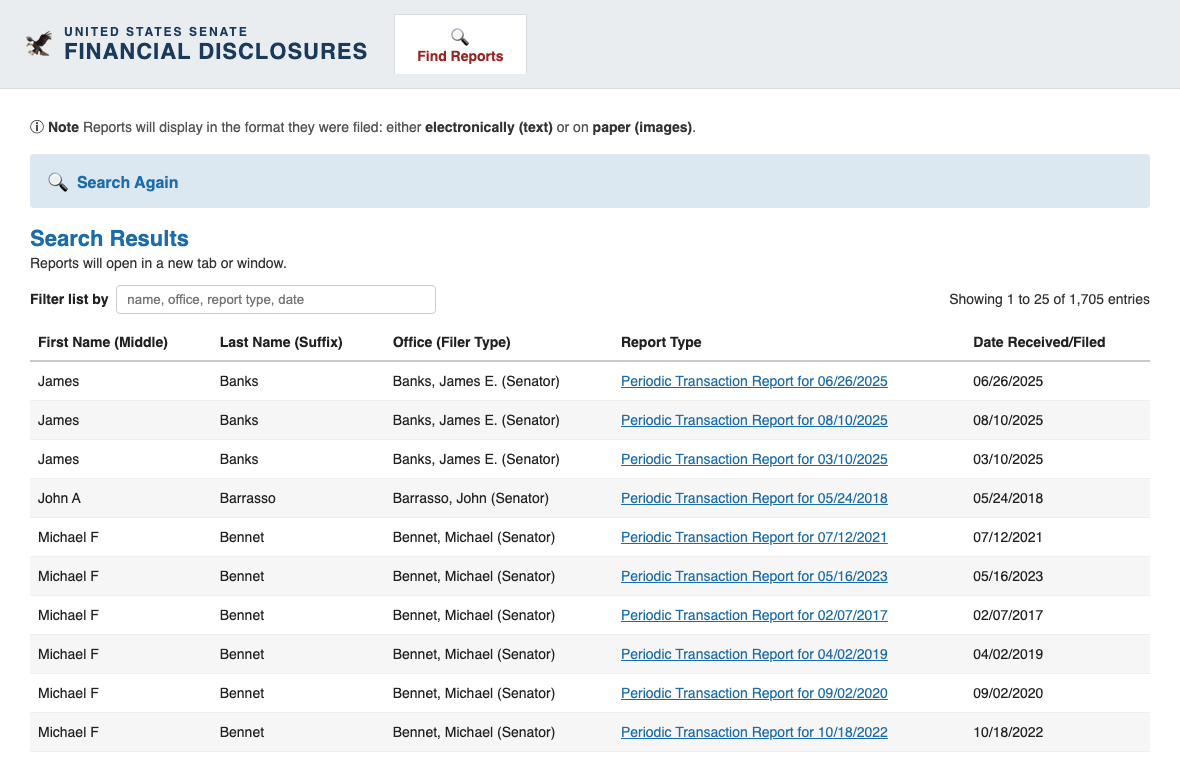
\includegraphics[width=0.90\linewidth]{slides/site_senate_results.png}}\\[0.5mm]
      {\scriptsize\color{black!60} la liste réelle : 1\,705 rapports « Sénateur × PTR »}
    \end{column}
    \begin{column}{0.46\textwidth}
      \colorbox{selec!12}{\parbox{0.96\linewidth}{\vspace{0.5mm}\footnotesize
        \textbf{Pourquoi ne prendre que les PTR ?}\\[1mm]
        {\scriptsize c'est \textbf{le} document des transactions (déclaré sous 45 j) ;
        les autres types n'apportent pas de trades exploitables :\\[1.2mm]
        · \textbf{Annual} — ne fait que \emph{résumer} les PTR (« \emph{Part 4a} »)\\[0.6mm]
        · \textbf{Blind Trust} — trades \textbf{non dirigés} par l'élu\\[0.6mm]
        · \textbf{Extension / Other} — administratif}\vspace{0.8mm}}}
    \end{column}
  \end{columns}
\end{frame}

% ── II.6 · Sénat électronique ── (vérifié sur les 1 777 HTML : UNE signature d'en-têtes 2014-2026)
\begin{frame}{Le chemin Sénat (2/5) — le cas électronique}
  \begin{columns}[T]
    \begin{column}{0.60\textwidth}\centering
      \fcolorbox{selec}{white}{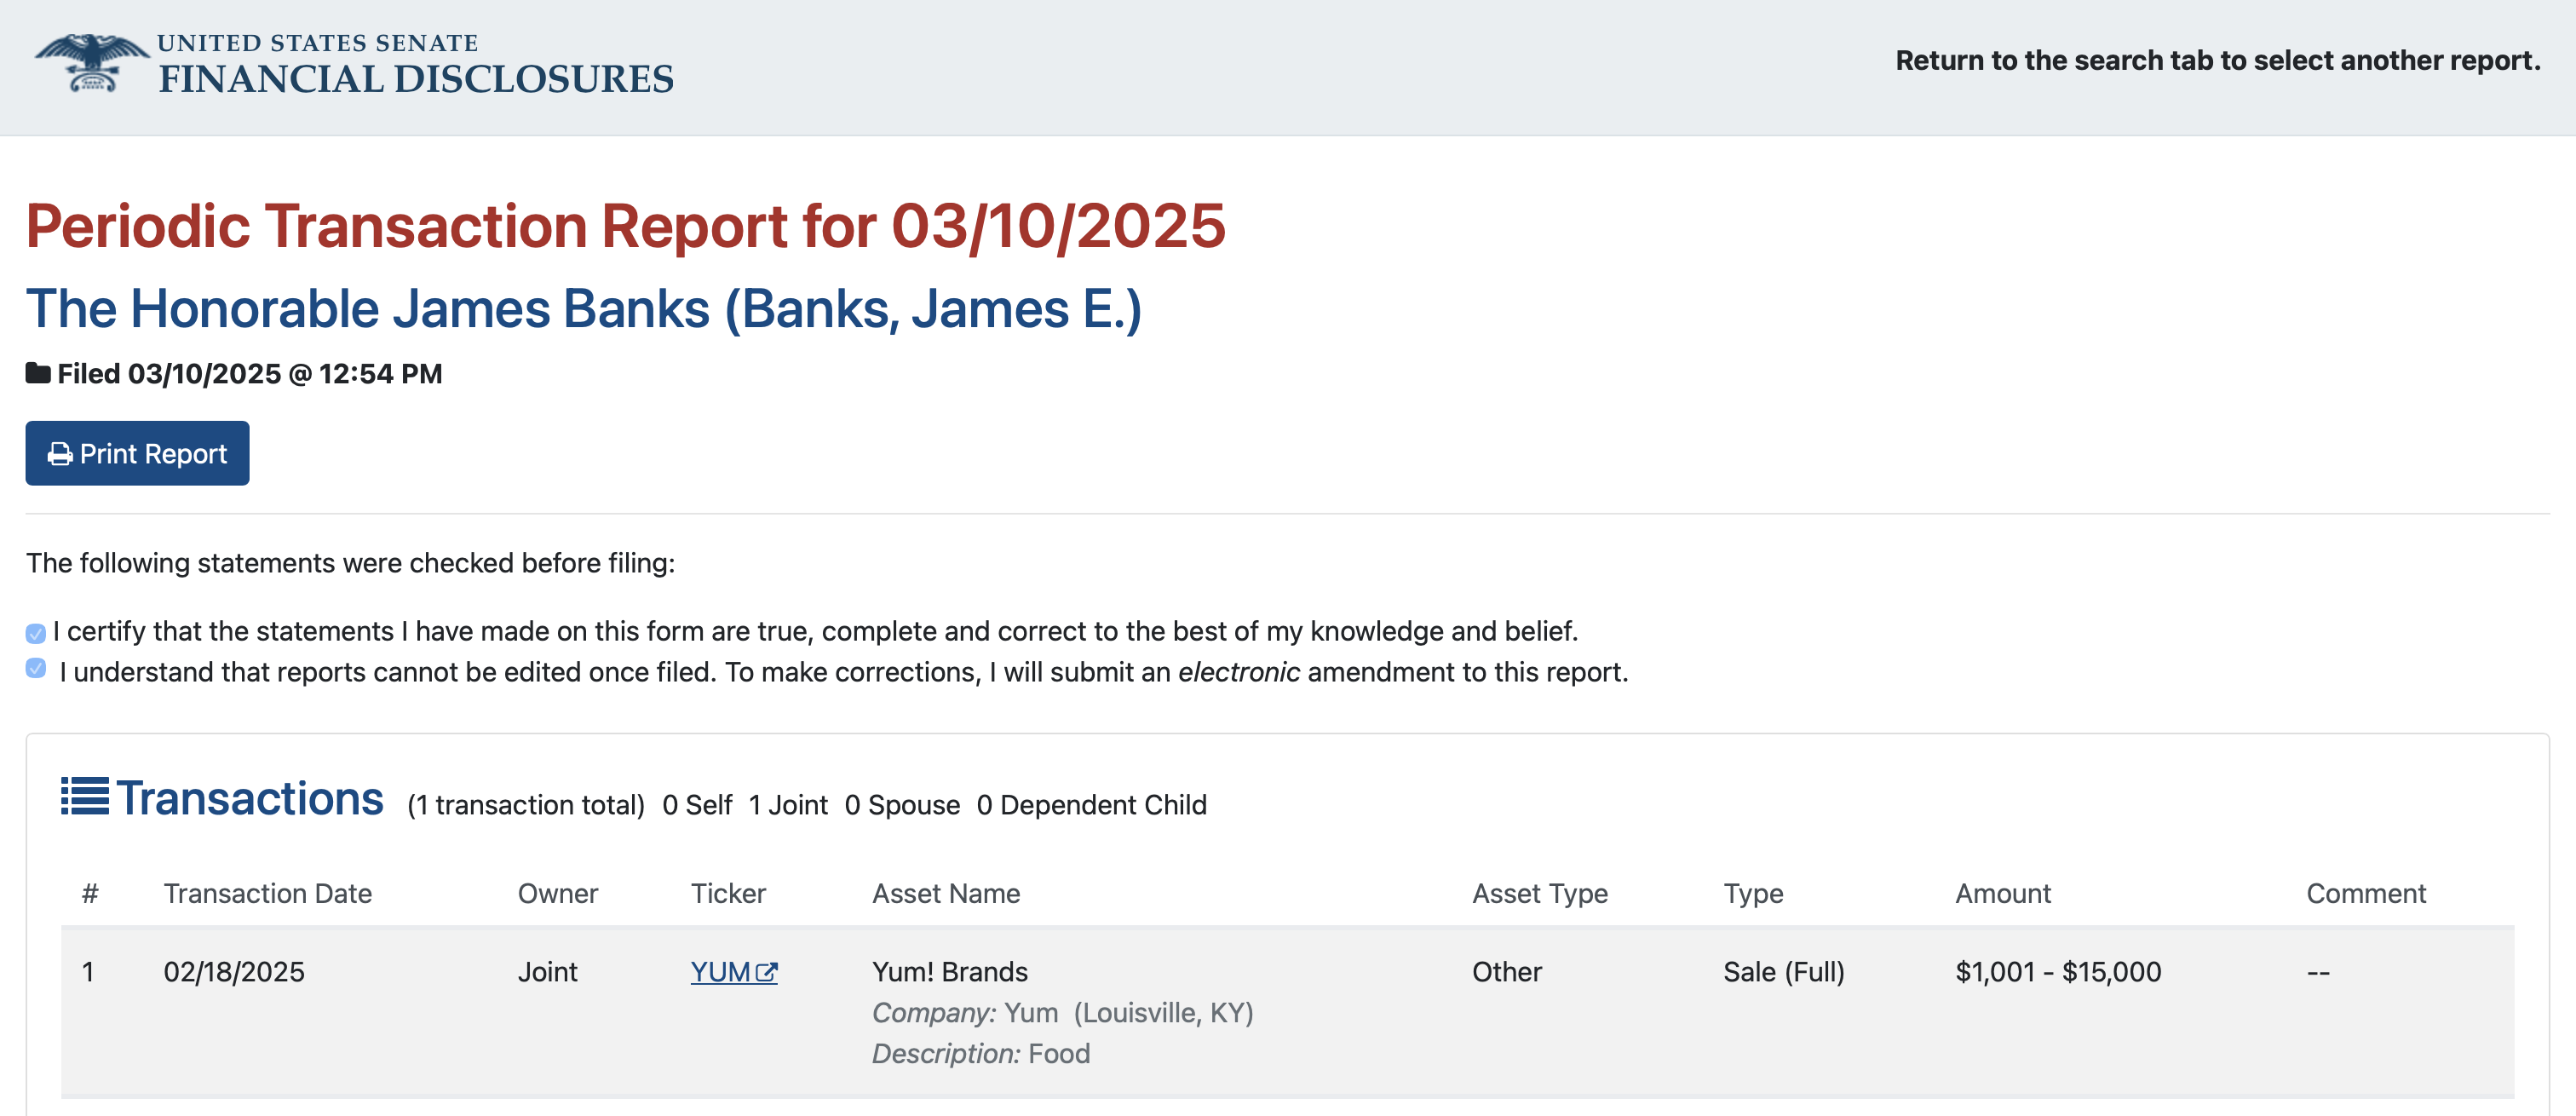
\includegraphics[width=\linewidth]{sources/senate_digital.png}}\\[0.5mm]
      {\scriptsize\color{black!60} une page web : table propre, ticker cliquable}
    \end{column}
    \begin{column}{0.38\textwidth}
      \badge{selec}{13\,026 transactions}\\[3mm]
      {\footnotesize les \textbf{9 mêmes colonnes} sur les \textbf{1\,777} rapports
       2014→2026 (vérifié) — \textbf{jamais} de changement de colonnes.}\\[2.5mm]
      {\footnotesize seul le \textbf{contenu} change :}\\[1.5mm]
      {\footnotesize
      · \textbf{amendements} (10\,\%)\\[1mm]
      · ticker « \co{--} » = \textbf{non-coté} (LLC, munis)\\[1mm]
      · cellules parfois vides (ex.\ \emph{Asset Type} en 2014)}
    \end{column}
  \end{columns}
\end{frame}

% ── II.7 · Sénat papier — le formulaire officiel ── (un seul modèle 2014-2026, couché/droit)
\begin{frame}{Le chemin Sénat (3/5) — le cas papier : le formulaire officiel}
  \centering
  {\footnotesize \textbf{un seul modèle} depuis 2014 (la grille A→L) — il arrive scanné
   couché ou droit :}\\[3mm]
  \begin{columns}[c]
    \begin{column}{0.42\textwidth}\centering
      \href{https://efd-media-public.senate.gov/media/2015/3/000/002/000002618.gif}{%
        \fcolorbox{black!30}{white}{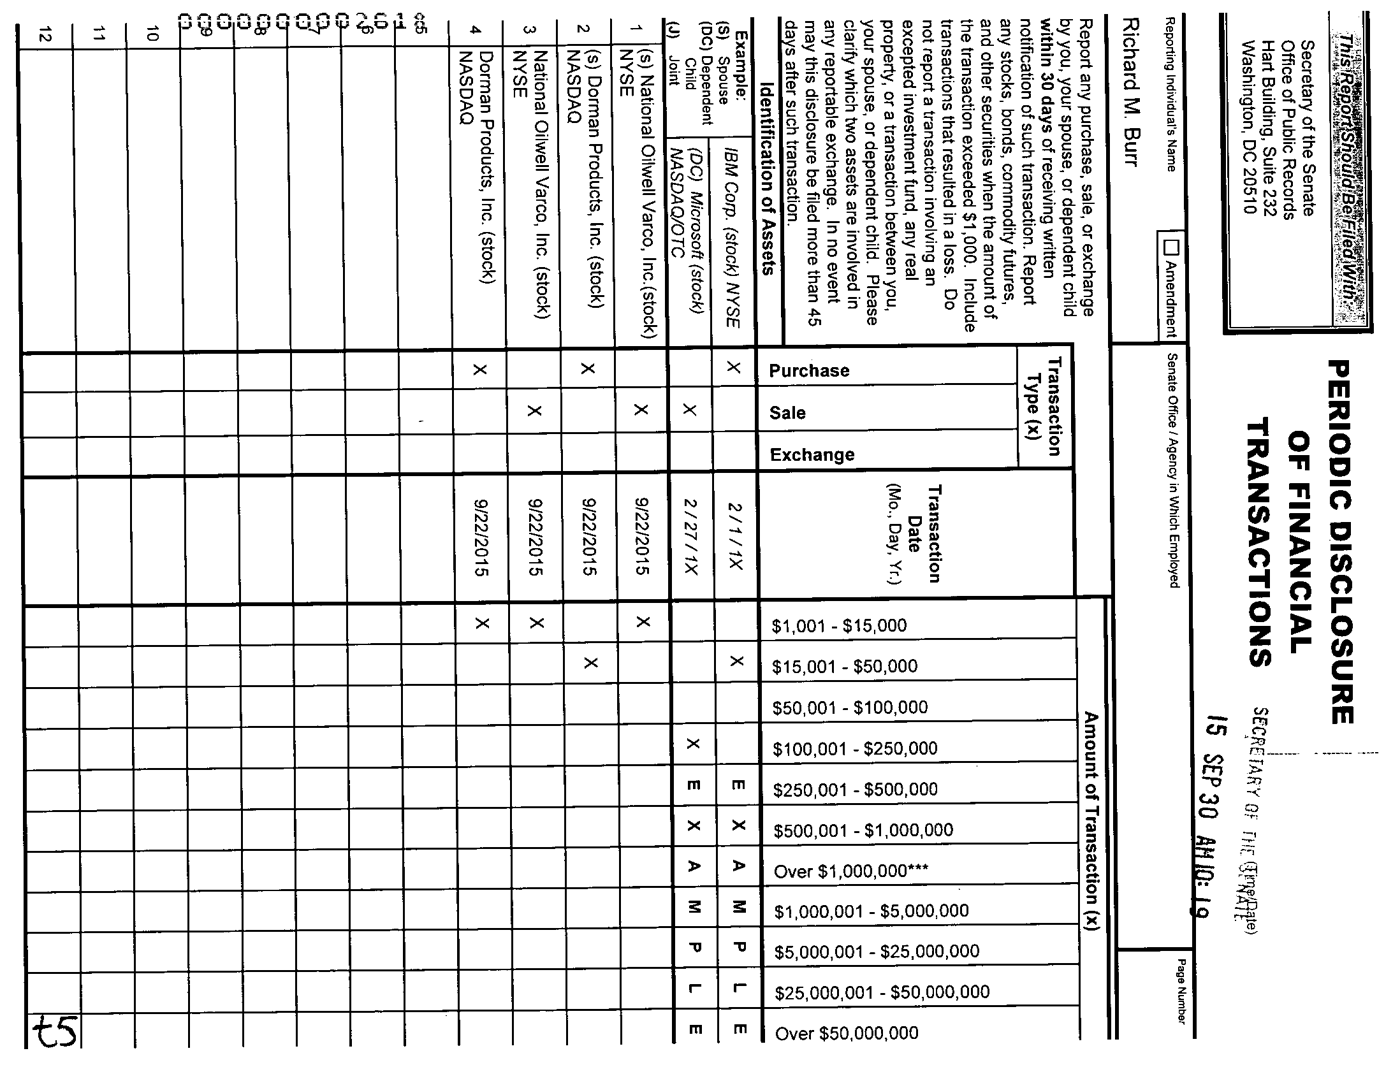
\includegraphics[height=47mm]{slides/senat_papier_couche.png}}}\\[1mm]
      {\scriptsize\textbf{couché} — 255/373 (à redresser avant lecture)}
    \end{column}
    \begin{column}{0.42\textwidth}\centering
      \href{https://efd-media-public.senate.gov/media/2020/2/000/000/000000936.gif}{%
        \fcolorbox{black!30}{white}{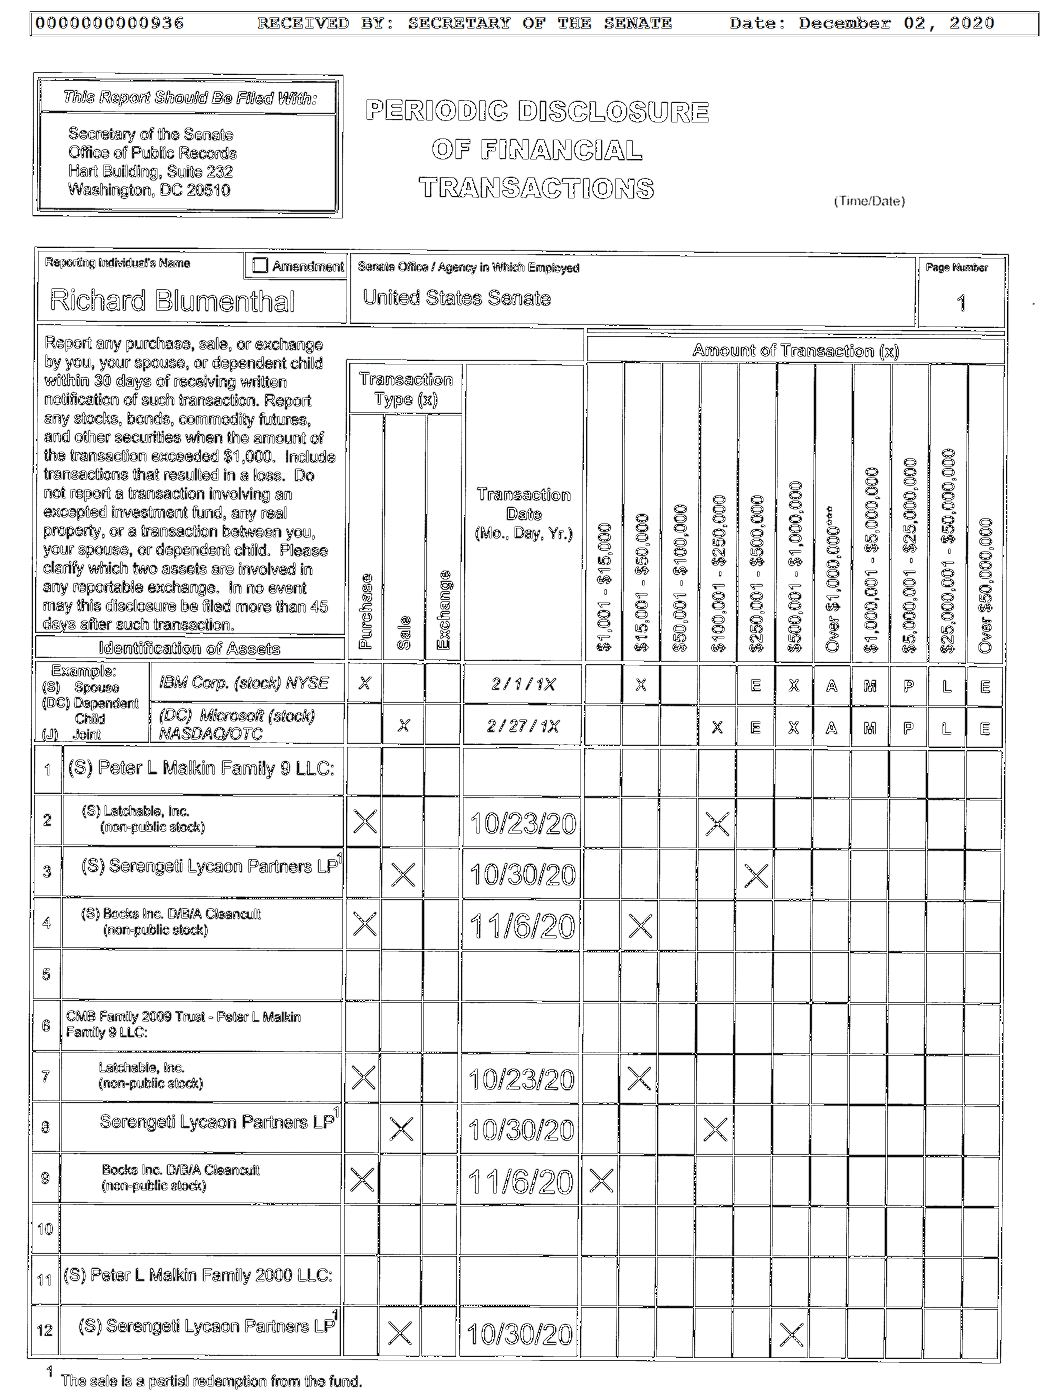
\includegraphics[height=47mm]{slides/senat_papier_droit.png}}}\\[1mm]
      {\scriptsize\textbf{droit} — le même formulaire}
    \end{column}
  \end{columns}
  \vspace{2mm}
  \badgel{socr}{3\,985 transactions}\quad
  {\scriptsize\color{black!60} parfois précédé d'une \textbf{page de garde} (lettre d'avocat /
   courrier) — p.1 sans données, ignorée · \textbf{cliquer = le vrai scan}}
\end{frame}

% ── II.7b · Sénat papier — remplissage ── (tapé le plus souvent ; manuscrit Roberts ; annexe Boozman)
\begin{frame}{Le chemin Sénat (4/5) — le même formulaire, trois remplissages}
  \centering
  {\footnotesize le plus souvent \textbf{tapé} — mais deux cas changent la difficulté d'OCR :}\\[3mm]
  \begin{columns}[c]
    \begin{column}{0.42\textwidth}\centering
      \href{https://efd-media-public.senate.gov/media/2014/1/000/012/000012036.gif}{%
        \fcolorbox{black!30}{white}{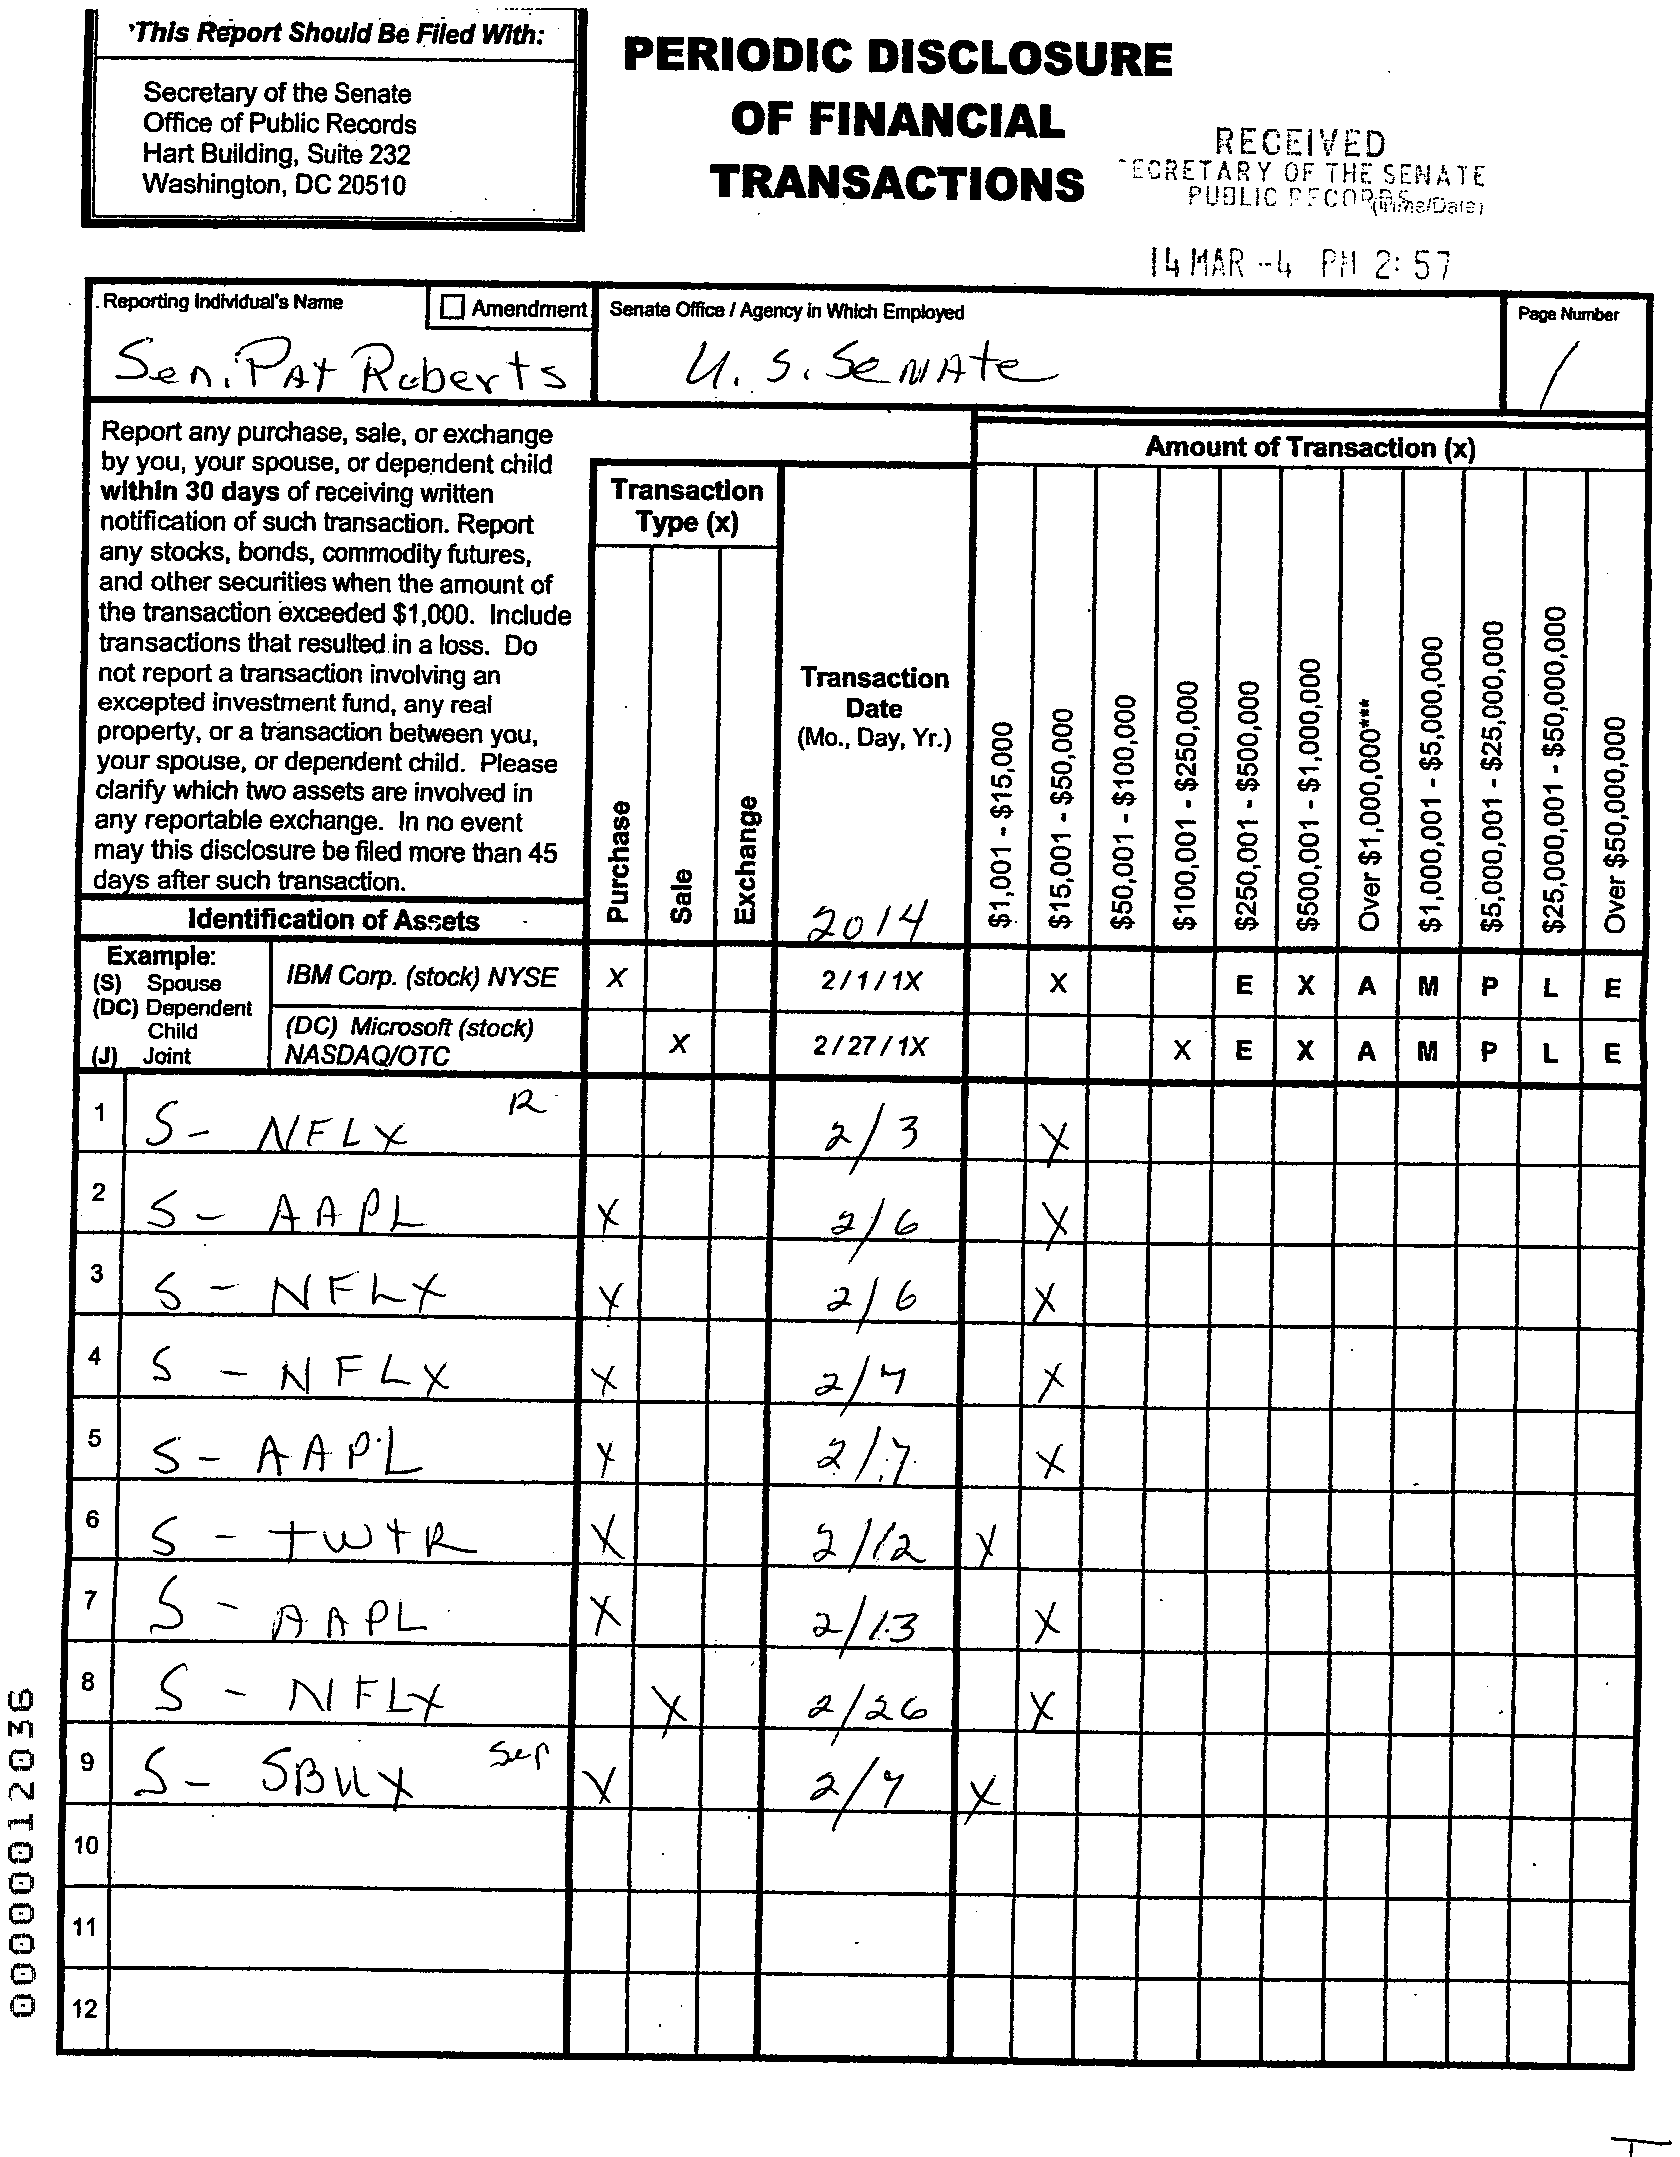
\includegraphics[height=48mm]{slides/senat_papier_manuscrit.png}}}\\[1mm]
      {\scriptsize\textbf{manuscrit} — rempli à la main (Roberts)\\dates et tickers plus durs à lire}
    \end{column}
    \begin{column}{0.42\textwidth}\centering
      \href{https://efd-media-public.senate.gov/media/2018/2/000/001/000001730.gif}{%
        \fcolorbox{black!30}{white}{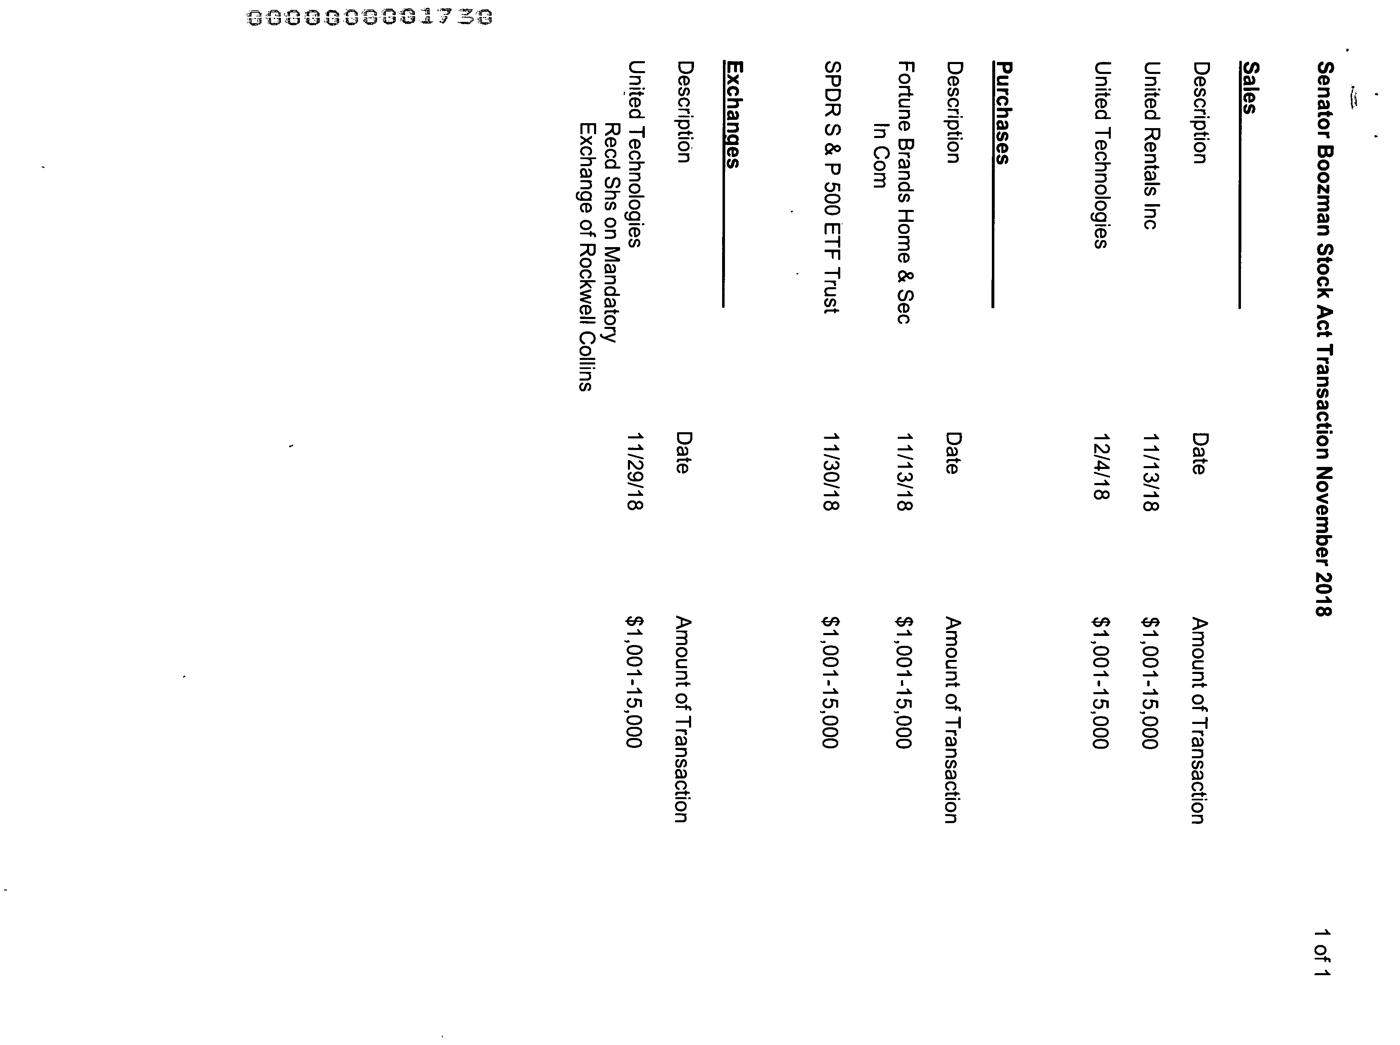
\includegraphics[height=48mm]{slides/senat_papier_annexe.png}}}\\[1mm]
      {\scriptsize\textbf{annexe « courtier »} — « See Attachment »\\→ une liste au format libre}
    \end{column}
  \end{columns}
  \vspace{2mm}
  {\scriptsize\color{black!60} \textbf{cliquer une vignette ouvre le vrai scan}}
\end{frame}

% ── II.7c · Sénat papier — les dates ── (dépôt = métadonnée eFD, jamais OCRisée ; txn = OCR + fenêtre
%    de plausibilité [dépôt-90j,+10j], senate/ocr.py:263 ; disclosure_date depuis le listing, l.136-142)
\begin{frame}{Le chemin Sénat (5/5) — les dates : deux natures, deux traitements}
  \begin{columns}[T]
    \begin{column}{0.48\textwidth}\centering
      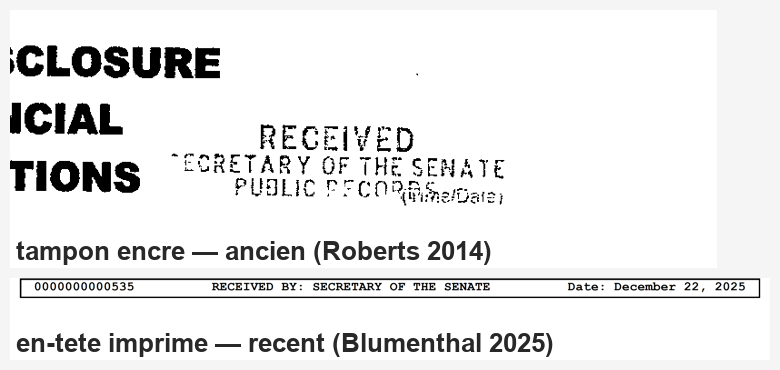
\includegraphics[width=\linewidth]{slides/fig_senat_date_depot.png}\\[1.5mm]
      \badge{okgreen}{date de dépôt → métadonnée eFD}\\[1.5mm]
      {\scriptsize écrite de façons variées (tampon encre, en-tête imprimé) — mais
       \textbf{jamais OCRisée} : on la lit sur la \textbf{fiche eFD}, donc fiable}
    \end{column}
    \begin{column}{0.48\textwidth}\centering
      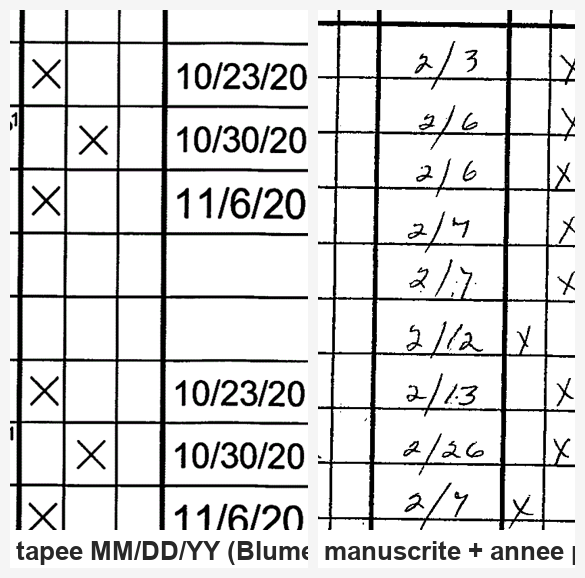
\includegraphics[height=40mm]{slides/fig_senat_date_txn.png}\\[1.5mm]
      \badge{warnorange}{date de transaction → OCRisée}\\[1.5mm]
      {\scriptsize formats variés (tapée · manuscrite · annexe) → garde-fou :
       fenêtre \textbf{[dépôt −90 j, +10 j]}}
    \end{column}
  \end{columns}
  \vspace{1mm}
  {\scriptsize\color{black!60}\centering → la date de la \textbf{divulgation}
   (celle de l'anti-look-ahead) est la fiable ; l'OCR ne touche qu'au trade}
\end{frame}

% ── II.8 · Les autres sources, en vrai ── (captures/extraits réels ; 100 334 wc cache)
\begin{frame}{Les autres sources, en vrai}
  \begin{columns}[T]
    \begin{column}{0.56\textwidth}\centering
      \fcolorbox{black!25}{white}{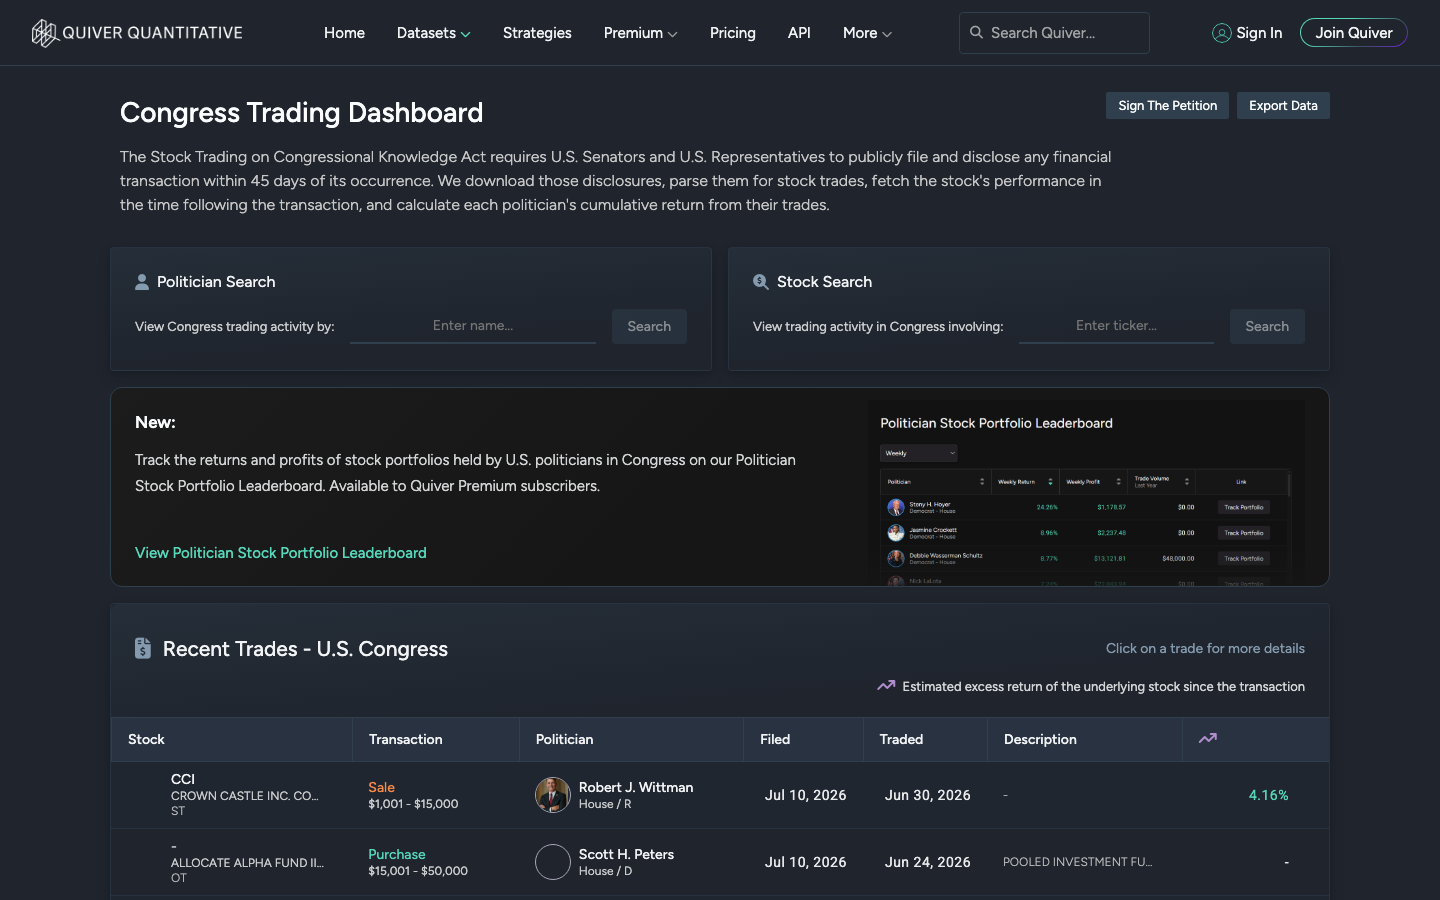
\includegraphics[width=0.82\linewidth]{slides/site_quiver.png}}\\[0.4mm]
      {\scriptsize\color{black!60} quiverquant.com (vérité-terrain externe)…}\\[0.8mm]
      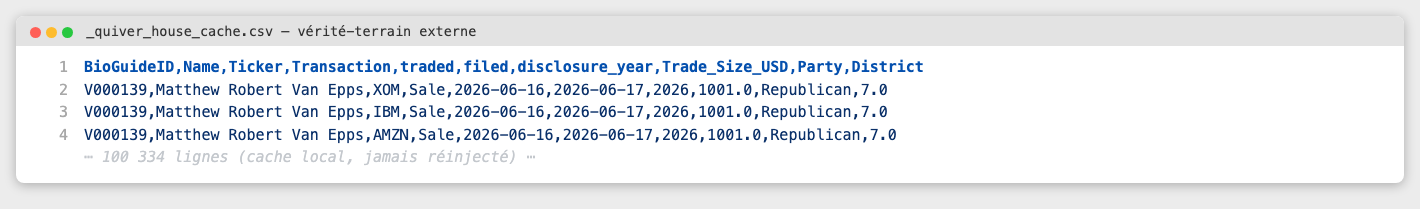
\includegraphics[width=0.88\linewidth]{slides/fichier_cache_quiver.png}\\[0.2mm]
      {\scriptsize\color{black!60} …et son export brut dans notre cache}
    \end{column}
    \begin{column}{0.42\textwidth}\centering
      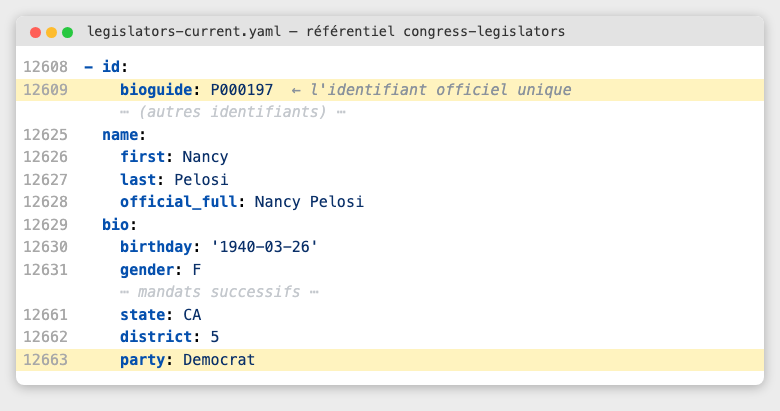
\includegraphics[width=\linewidth]{slides/fichier_referentiel_yaml.png}\\[0.4mm]
      {\scriptsize\color{black!60} le référentiel d'identité \emph{congress-legislators}
       (nom → \co{bioguide\_id}, parti, mandats)}\\[3mm]
      \colorbox{black!6}{\parbox{0.95\linewidth}{\footnotesize\centering
        ces sources servent à \textbf{identifier} et à \textbf{mesurer} —\\
        \textbf{jamais réinjectées} dans nos tables}}
    \end{column}
  \end{columns}
\end{frame}

% ═════════════ III. LE FLUX ═════════════
\section{Le flux de bout en bout}

% ── S8 · Flux de bout en bout ── (adaptation 16:9 du diagramme §3.2 de RAPPORT_FINAL.tex l.228-278)
\begin{frame}{Le flux de bout en bout}
  \centering
  \resizebox{!}{0.88\textheight}{%
  \begin{tikzpicture}[node distance=3mm]
    % Acquisition (2 racines)
    \node[step=dataC, text width=6.2cm] (acqH) at (-3.7,0)
      {\textbf{\color{helec}Chambre} — \emph{House Clerk} → index XML → PDF};
    \node[step=dataC, text width=6.2cm] (acqS) at (3.7,0)
      {\textbf{\color{selec}Sénat} — \emph{eFD} → liste des dépôts (HTML ou papier)};
    % Tri
    \node[step=helec, text width=2.9cm] (hpdf) at (-5.5,-1.35) {\textbf{PDF lisible}\\couche texte présente};
    \node[step=helec, text width=2.9cm] (hscan) at (-2.0,-1.35) {\textbf{scan tapé}\\image, souvent couchée};
    \node[step=selec, text width=2.9cm] (shtml) at (2.0,-1.35) {\textbf{page HTML}\\déclaration eFD};
    \node[step=selec, text width=2.9cm] (sgif) at (5.5,-1.35) {\textbf{image papier}\\\co{.gif}, déjà droite};
    \node[step=alertred, text width=2.9cm, font=\tiny] (hC) at (-2.0,-2.5)
      {scan \textbf{manuscrit} → écarté (politique rejouable)};
    % Extraction
    \node[step=helec, text width=2.9cm] (hpar) at (-5.5,-2.75)
      {\textbf{parsing déterministe}\\[0.5mm]{\normalsize\textbf{\color{helec}58\,728}}};
    \node[step=helec, text width=2.9cm] (hvis) at (-2.0,-3.65)
      {\textbf{OCR Claude Vision} redressée, lue en JSON\\[0.5mm]{\normalsize\textbf{\color{helec}93\,261}}};
    \node[step=selec, text width=2.9cm] (spar) at (2.0,-2.75)
      {\textbf{lecture des tableaux}\\appariement flou\\[0.5mm]{\normalsize\textbf{\color{selec}13\,026}}};
    \node[step=selec, text width=2.9cm] (svis) at (5.5,-2.75)
      {\textbf{OCR Claude Vision}\\image déjà droite\\[0.5mm]{\normalsize\textbf{\color{selec}3\,985}}};
    % Tronc commun
    \node[bande=grisC, text width=13.6cm] (conv) at (0,-4.85)
      {\textbf{lignes normalisées} — déclarant, dates (trade + divulgation), actif, opération,
       fourchette, détenteur \emph{(les 7 champs de la clé naturelle)}};
    \node[bande=grisC, text width=13.6cm] (ident) at (0,-5.75)
      {\textbf{identité} — nom libre → \co{bioguide\_id} officiel (+ parti, commissions) via le référentiel partagé};
    \node[bande=grisC, text width=13.6cm] (enr) at (0,-6.65)
      {\textbf{enrichissement} — ticker (explicite → dictionnaire → LLM → récupération) ·
       secteur \textbf{GICS → ETF SPDR} · montant → \emph{milieu} · ancienneté};
    \node[bande=dataC, fill=dataC!14, text width=13.6cm] (fin) at (0,-7.55)
      {\textbf{TABLE FINALE} — \textbf{169\,000 uniques} (170\,920 lignes) ·
       \co{06\_\{ch\}\_\{an\}\_FINAL.csv} · 28 colonnes · contrat 12 champs métier};
    \node[bande=alertred, text width=13.6cm] (val) at (0,-8.45)
      {\textbf{validation} — Quiver (3 niveaux : existence / date / champs) + sources indépendantes
       + golden — \textbf{jamais réinjectées}};
    \node[bande=dataC, fill=dataC!14, text width=13.6cm] (clean) at (0,-9.35)
      {\textbf{TABLE DE RECHERCHE} — \textbf{134\,464 × 36} ·
       \co{data/clean/transactions\_backtest\_2014\_2026.csv} · entonnoir A→D + point-in-time};
    % Bandes latérales
    \node[font=\tiny\bfseries, text=gray!60, rotate=90] at (-7.6,0) {Acquisition};
    \node[font=\tiny\bfseries, text=gray!60, rotate=90] at (-7.6,-1.4) {Tri};
    \node[font=\tiny\bfseries, text=gray!60, rotate=90] at (-7.6,-3.2) {Extraction};
    \node[font=\tiny\bfseries, text=gray!60, rotate=90] at (-7.6,-5.75) {Tronc commun};
    \node[font=\tiny\bfseries, text=gray!60, rotate=90] at (-7.6,-8.9) {Livraison};
    % Flèches
    \draw[arr] (acqH) -- (hpdf); \draw[arr] (acqH) -- (hscan);
    \draw[arr] (acqS) -- (shtml); \draw[arr] (acqS) -- (sgif);
    \draw[arr] (hscan) -- (hC);
    \draw[arr] (hpdf) -- (hpar); \draw[arr] (hscan) -- (hvis);
    \draw[arr] (shtml) -- (spar); \draw[arr] (sgif) -- (svis);
    \draw[arr] (hpar.south) -- (conv.north -| hpar.south);
    \draw[arr] (hvis.south) -- (conv.north -| hvis.south);
    \draw[arr] (spar.south) -- (conv.north -| spar.south);
    \draw[arr] (svis.south) -- (conv.north -| svis.south);
    \draw[arr] (conv) -- (ident); \draw[arr] (ident) -- (enr); \draw[arr] (enr) -- (fin);
    \draw[arr] (fin) -- (val); \draw[arr] (val) -- (clean);
  \end{tikzpicture}}
\end{frame}

% ═════════════ IV. CONSTRUCTION, ÉTAPE PAR ÉTAPE ═════════════
\section{Construction de la donnée, étape par étape}

% ── S9 · Identité ── (RAPPORT_FINAL §4.1 ; 100 %/367/78 RQ §1 ; Casey/Craig AUDIT §4)
\begin{frame}{Étape 1 — d'abord, savoir qui a déclaré (identité)}
  \begin{columns}[T]
    \begin{column}{0.58\textwidth}
      {\footnotesize le même élu signe « Hon.\ Earl L.\ Carter », « Buddy Carter »,
       « N.\ Pelosi »… → il faut un \textbf{identifiant unique}}\\[2mm]
      \centering
      \begin{tikzpicture}[node distance=2.6mm]
        \node[step=grisC, text width=6.6cm] (n) {\textbf{nom libre du formulaire}};
        \node[step=helec, text width=6.6cm, below=of n] (c1)
          {1. \textbf{override manuel} — un seul cas par chambre (Van Taylor · J.D.\ Vance)};
        \node[step=helec, text width=6.6cm, below=of c1] (c2)
          {2. \textbf{correspondance exacte} — accents, titres (\emph{Hon., Dr.}),
           suffixes, diminutifs (\emph{William → Bill})};
        \node[step=helec, text width=6.6cm, below=of c2] (c3)
          {3. \textbf{repli nom de famille} (s'il ne désigne qu'un élu) —
           au Sénat : + désambiguïsation (siège, titulaire en exercice)};
        \node[step=okgreen, text width=6.6cm, below=of c3] (r)
          {\co{bioguide\_id} officiel → \textbf{parti + commissions} joints};
        \draw[arr] (n) -- (c1); \draw[arr] (c1) -- (c2);
        \draw[arr] (c2) -- (c3); \draw[arr] (c3) -- (r);
      \end{tikzpicture}
    \end{column}
    \begin{column}{0.40\textwidth}
      \badge{okgreen}{100\,\% des lignes rattachées}\\[1mm]
      {\footnotesize \textbf{367} membres Chambre · \textbf{78} Sénat}\\[3mm]
      {\footnotesize\textbf{Pièges réels, réparés :}}\\[1mm]
      {\scriptsize
      · homonymie : le sénateur Bob Casey rattaché à tort à \co{C000228}
        (un représentant texan) → \co{C001070}\\[1mm]
      · \textbf{42 lignes} d'Angie Craig sans identifiant → réparées (read-time, figé intact)\\[1mm]
      · 1 seule déclaration \textbf{exclue} : une collaboratrice de commission
        (pas un élu — vérifié au PDF)}
    \end{column}
  \end{columns}
\end{frame}

% ── S10 · Tri des formats ── (§4.2 ; parts RQ §1)
\begin{frame}{Étape 2 — trier : électronique ou scanné ?}
  \centering
  \begin{tikzpicture}[node distance=3.5mm]
    \node[step=helec, text width=5.2cm] (h) {\textbf{Chambre} : le format n'est pas annoncé
      → on ouvre chaque PDF (\co{pdfplumber}) et on teste la \textbf{couche texte}
      (\co{bool(text.strip())})};
    \node[step=selec, text width=5.2cm, right=14mm of h] (s) {\textbf{Sénat} : le portail
      \textbf{annonce le type} de chaque dépôt (\co{ptr} électronique / \co{paper} scanné)};
    \node[step=grisC, text width=5.2cm, below=6mm of $(h.south)!0.5!(s.south)$] (f)
      {\textbf{la fourche du pipeline} — ce tri fixe la composition finale du corpus
       et route chaque document vers sa piste};
    \draw[arr] (h) -- (f); \draw[arr] (s) -- (f);
  \end{tikzpicture}

  \vspace{5mm}
  % Composition (parts RQ §1) — barre 100 % faite en tikz
  {\footnotesize la composition qui en résulte (169\,000 transactions uniques) :}\\[1.5mm]
  \begin{tikzpicture}
    \draw[fill=helec, draw=none] (0,0) rectangle (4.176,0.55);
    \draw[fill=hocr, draw=none] (4.176,0) rectangle (10.8,0.55);
    \draw[fill=selec, draw=none] (10.8,0) rectangle (11.724,0.55);
    \draw[fill=socr, draw=none] (11.724,0) rectangle (12.0,0.55);
    \node[font=\scriptsize, color=white] at (2.09,0.275) {\textbf{élec.\ 34,8\,\%}};
    \node[font=\scriptsize, color=black!75] at (7.5,0.275) {\textbf{Chambre OCR 55,2\,\%}};
    \node[font=\tiny, color=white] at (11.26,0.275) {\textbf{7,7}};
    \node[font=\tiny, color=black!75, above=1mm of {(11.86,0.55)}] {Sénat OCR 2,4\,\%};
  \end{tikzpicture}\\[1mm]
  {\scriptsize\color{black!60} plus de la moitié du corpus vient de \textbf{scans} —
   le papier n'est pas un détail, c'est la majorité}
\end{frame}

% ── S11 · Piste électronique Chambre ── (§4.3 ; pièges digital.py:305-345 ; 102 §4.3)
\begin{frame}{Étape 3 — la piste électronique de la Chambre}
  \badge{helec}{58\,728 transactions uniques}\quad
  {\footnotesize\color{black!60} zéro échec silencieux : tout PDF sans ligne est consigné
   (\co{05\_parse\_failures}) — 102 « nothing to report » réels}\\[3mm]
  \begin{columns}[T]
    \begin{column}{0.55\textwidth}
      \centering
      \begin{tikzpicture}[node distance=3mm]
        \node[step=grisC, text width=6.2cm] (a)
          {le PDF ne donne pas un tableau régulier : une transaction s'étale
           sur \textbf{plusieurs lignes}, montants coupés};
        \node[step=helec, text width=6.2cm, below=of a] (b)
          {\textbf{1. recoller} les lignes coupées (\co{\_join\_split\_lines})};
        \node[step=helec, text width=6.2cm, below=of b] (c)
          {\textbf{2. repérer la signature} de chaque transaction :
           opération (P/S/E) + \textbf{2 dates} + fourchette};
        \node[step=helec, text width=6.2cm, below=of c] (d)
          {\textbf{3. rattacher} actif et ticker imprimés à proximité};
        \draw[arr] (a) -- (b); \draw[arr] (b) -- (c); \draw[arr] (c) -- (d);
      \end{tikzpicture}
    \end{column}
    \begin{column}{0.43\textwidth}
      \colorbox{alertred!10}{\parbox{0.96\linewidth}{\footnotesize
        \textcolor{alertred}{\textbf{Pièges déjoués}}\\[1mm]
        {\scriptsize
        · le \textbf{gabarit change en 2018} (casse, codes, mise en page) →
          \textbf{deux parseurs} routés par signature, union dédupliquée ;
          sans ça, ≈\,\textbf{72 ventes} perdues rien qu'en 2014 (biais vendeur)\\[1mm]
        · \textbf{205 PTR} déposés après le 31/12 étaient perdus →
          l'index annuel du Clerk fait désormais \textbf{autorité}}}}\\[3mm]
      {\scriptsize dans la source :\\
       \colorbox{black!6}{\parbox{0.94\linewidth}{\ttfamily\scriptsize
        Amazon.com, Inc.\ — Common Stock \textbf{(AMZN)} [ST] · Purchase ·
        03/16/2018 · \$1,001--\$15,000}}}
    \end{column}
  \end{columns}
\end{frame}

% ── S12 · Piste électronique Sénat ── (§4.4)
\begin{frame}{Étape 4 — la piste électronique du Sénat}
  \badge{selec}{13\,026 transactions uniques}\\[3mm]
  \centering
  \resizebox{\textwidth}{!}{%
  \begin{tikzpicture}[node distance=3.5mm]
    \node[step=selec, text width=3.6cm] (a) {\textbf{liste des dépôts}\\recherche paginée
      (type PTR), barrière CSRF passée};
    \node[step=selec, text width=3.6cm, right=of a] (b) {\textbf{page HTML par dépôt}\\
      mise en cache disque — un re-run ne retélécharge rien};
    \node[step=selec, text width=3.6cm, right=of b] (c) {\textbf{lecture des tableaux}\\
      \co{pd.read\_html} → DataFrames bruts};
    \node[step=selec, text width=3.6cm, right=of c] (d) {\textbf{colonnes repérées}\\
      par mots-clés (« ticker », « asset », « name »)};
    \draw[arr] (a) -- (b); \draw[arr] (b) -- (c); \draw[arr] (c) -- (d);
  \end{tikzpicture}}

  \vspace{5mm}
  \colorbox{black!6}{\parbox{0.85\textwidth}{\footnotesize\centering
    on repère chaque colonne par son mot-clé \textbf{par robustesse} — mais en pratique
    le gabarit est \textbf{stable} : les mêmes \textbf{9 colonnes} sur les 1\,777 rapports
    2014→2026 (vérifié)}}\\[3mm]
  {\scriptsize\color{black!60} identité, ticker et déduplication : délégués au tronc commun
   — même clé naturelle que la Chambre}
\end{frame}

% ── S13 · Piste scannée Chambre (OCR) ── (§4.5 ; census vérifié awk ; 12,9 % RQ §6.6)
\begin{frame}{Étape 5 — la piste scannée de la Chambre (OCR Vision)}
  \centering
  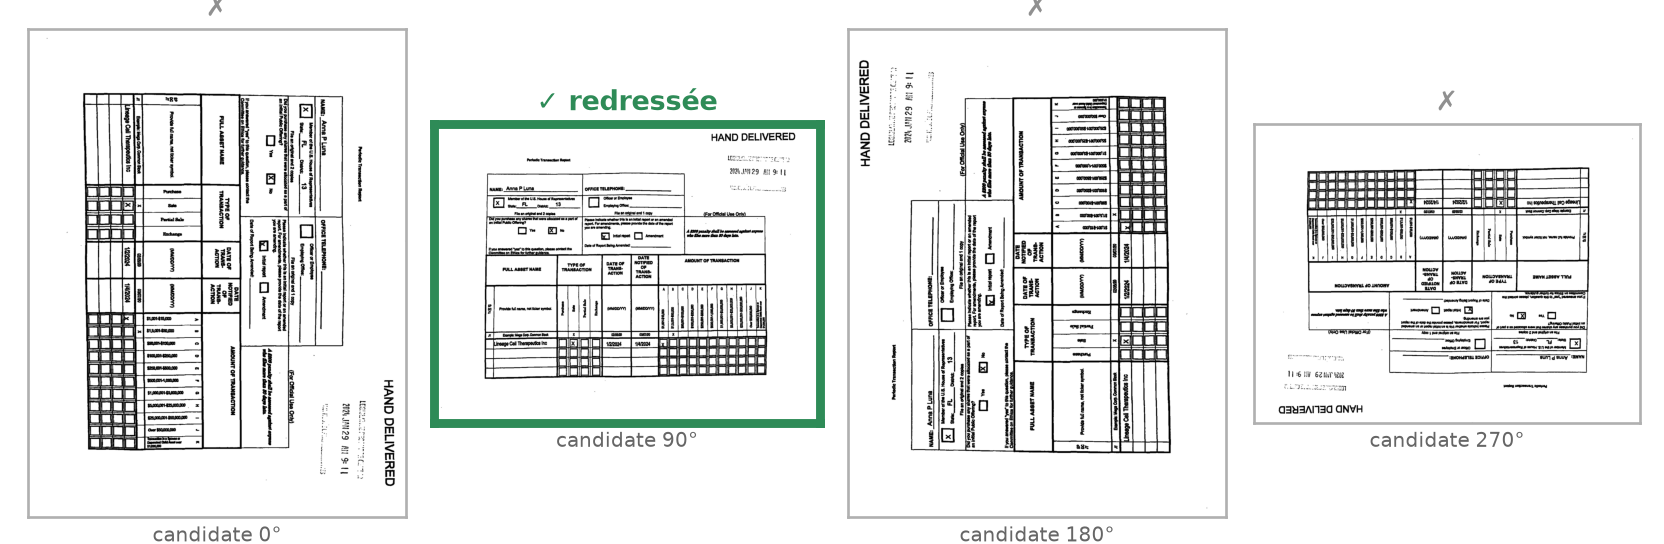
\includegraphics[width=0.70\textwidth]{slides/fig_deskew_rotations.png}

  \vspace{1mm}
  \begin{columns}[T]
    \begin{column}{0.46\textwidth}\footnotesize
      \textbf{1.} redresser — reconnaissance d'orientation (4 candidates)\\[0.8mm]
      \textbf{2.} classer — census \textbf{2\,424 scans} : 74 droits ·
        1\,575 tournés · \textbf{775 manuscrits}\\[0.8mm]
      \textbf{3.} lire — \co{tool\_use} forcé, JSON strict, \textbf{cache versionné}
        (un re-run ne re-paie rien), prompt durci sur échantillon
    \end{column}
    \begin{column}{0.52\textwidth}\footnotesize
      \colorbox{alertred!10}{\parbox{0.97\linewidth}{\scriptsize
        \textbf{\textcolor{alertred}{gating manuscrit}} — Quiver ne corrobore que
        \textbf{12,9\,\%} du manuscrit (88\,\% du tapé droit) : dates cursives trop
        incertaines → \textbf{582 écartés}, règle écrite \textbf{rejouable},
        exceptions explicites (3 déposants + 33 docs curés)}}\\[1.5mm]
      \badgel{hocr}{93\,261 lignes — très concentrées}\\[1mm]
      {\scriptsize Khanna à lui seul \textbf{44,0\,\%} · trio Khanna, McCaul,
       Harshbarger \textbf{77,1\,\%} — de gros déposants qui déclarent
       \textbf{exclusivement sur papier}}
    \end{column}
  \end{columns}
\end{frame}

% ── S14 · Piste papier Sénat ── (§4.6 ; JSON Boozman = ocr_cache réel)
\begin{frame}[fragile]{Étape 6 — la piste papier du Sénat}
  \begin{columns}[T]
    \begin{column}{0.50\textwidth}
      \badgel{socr}{3\,985 lignes — 14 déposants}\\[2mm]
      {\footnotesize
      · images \textbf{déjà droites} : pas de redressement, même moteur Vision\\[1mm]
      · particularité : fusion + enrichissement \textbf{en une passe sur tout le corpus}
        (peu de données par année → le dictionnaire de tickers est mutualisé
        entre les années)\\[1mm]
      · Blumenthal = \textbf{38,7\,\%} de la piste ; massivement du
        \textbf{non-coté} (munis, produits structurés) → couverture ticker
        plus basse = \textbf{composition, pas défaut d'extraction}}
    \end{column}
    \begin{column}{0.48\textwidth}
      {\scriptsize ce que rend l'OCR (extrait réel — John Boozman) :}
\begin{Verbatim}[fontsize=\scriptsize, frame=single, rulecolor=\color{black!25}]
{ "member": "JOHN BOOZMAN",
  "status": "ok", "n_pages": 2,
  "transactions": [
   { "asset_description":
       "Apple Computer Inc",
     "transaction_type": "Sale",
     "owner": "Self",
     "transaction_date": "2022-03-14",
     "amount_code": "A" }, ... ] }
\end{Verbatim}
    \end{column}
  \end{columns}
\end{frame}

% ── S15 · Secteur GICS→ETF ── (§4.7)
\begin{frame}{Étape 7 — un secteur pour chaque ticker : GICS → ETF SPDR}
  \begin{columns}[T]
    \begin{column}{0.52\textwidth}\footnotesize
      \textbf{résoudre le ticker} (cascade, source tracée) :\\[1mm]
      \begin{tikzpicture}[node distance=2.2mm]
        \node[bande=helec, text width=6.4cm] (t1) {1. \textbf{explicite} — déjà imprimé dans la source};
        \node[bande=helec, text width=6.4cm, below=of t1] (t2) {2. \textbf{dictionnaire} — nom vu ailleurs dans le corpus};
        \node[bande=helec, text width=6.4cm, below=of t2] (t3) {3. \textbf{LLM} filtré « action » — jamais d'obligation/muni tickerisée};
        \node[bande=okgreen, text width=6.4cm, below=of t3] (t4) {4. \textbf{récupération} validée par double preuve — \textbf{2\,540 lignes} retrouvent leur symbole};
        \draw[arr] (t1) -- (t2); \draw[arr] (t2) -- (t3); \draw[arr] (t3) -- (t4);
      \end{tikzpicture}\\[2mm]
      \textbf{puis le secteur} : yfinance (factuel) → LLM contraint GICS
      (+ garde-fou \co{is\_listed}) → overrides manuels
    \end{column}
    \begin{column}{0.46\textwidth}\footnotesize
      \textbf{11 secteurs GICS → 11 ETF} \emph{Select Sector SPDR} :\\[1.5mm]
      {\scriptsize\ttfamily
      Energy→XLE · Materials→XLB · Industrials→XLI · Cons.\ Discr.→XLY ·
      Cons.\ Staples→XLP · Health Care→XLV · Financials→XLF · Info.\ Tech.→XLK ·
      Comm.\ Services→XLC · Utilities→XLU · Real Estate→XLRE}\\[3mm]
      \colorbox{black!6}{\parbox{0.96\linewidth}{\scriptsize
        \textbf{couverture = remplissage, pas exactitude} : ticker renseigné
        \textbf{84,1\,\%} Chambre / \textbf{77,9\,\%} Sénat ; secteur
        \textbf{79,8\,\%} / \textbf{70,4\,\%} — les vides sont le
        \textbf{non-coté légitime} (munis, obligations, fonds privés),
        pas des défauts d'extraction}}
    \end{column}
  \end{columns}
\end{frame}

% ── S16 · Table finale ── (§4.8)
\begin{frame}{Étape 8 — la table finale : le contrat « 12/12 »}
  \begin{columns}[T]
    \begin{column}{0.55\textwidth}\footnotesize
      \textbf{une clé naturelle de 7 champs} :\\
      {\scriptsize déclarant · date du trade · actif · opération · fourchette ·
       détenteur · chambre}\\[1.5mm]
      {\scriptsize elle exclut \textbf{délibérément} :\\
       · le \textbf{ticker} — ajouté plus tard (enrichissement), sa présence rendrait
         la clé instable\\
       · la \textbf{date de divulgation} — un dépôt et son amendement portent le
         \emph{même} trade → une seule transaction}\\[2mm]
      \textbf{dédup non destructrice} :\\
      {\scriptsize · les \textbf{lots réels} (même titre déclaré plusieurs fois dans un
        dépôt, comptes Self/Spouse/Joint) sont \textbf{préservés}
        (\co{occurrence\_index}) — jamais de \co{drop\_duplicates()} aveugle\\
       · \textbf{dédup cross-année} : une re-divulgation (amendement, rapport annuel)
        ne compte qu'une fois → \textbf{−1\,920}}
    \end{column}
    \begin{column}{0.43\textwidth}
      \centering
      \begin{tikzpicture}[node distance=3mm]
        \node[bande=grisC, text width=4.9cm] (a) {\textbf{170\,920} lignes brutes\\(26 fichiers FINAL, 28 colonnes)};
        \node[bande=grisC, text width=4.9cm, below=of a] (b) {dédup cross-année \textbf{−1\,920}};
        \node[bande=dataC, fill=dataC!14, text width=4.9cm, below=of b] (c)
          {\textbf{169\,000 transactions uniques}};
        \draw[arr] (a) -- (b); \draw[arr] (b) -- (c);
      \end{tikzpicture}\\[3mm]
      \colorbox{helec}{\parbox{0.9\linewidth}{\footnotesize\color{white}\centering
        \textbf{12 champs métier garantis} sur les 2 chambres : qui, quoi, quand
        (2 dates), sens, montant, ticker, secteur, ETF, parti, commissions}}
    \end{column}
  \end{columns}
\end{frame}

% ═════════════ V. VALIDATION ═════════════
\section{Validation}

% ── S17 · Quiver N1 ── (RQ §6.1-6.2)
\begin{frame}{Validation (1/3) — Quiver, niveau 1 : a-t-on tout ?}
  \begin{columns}[T]
    \begin{column}{0.33\textwidth}
      {\footnotesize \textbf{la méthode} : chaque trade confronté à Quiver par clé
       normalisée (élu × ticker × sens), en \textbf{3 niveaux de strictesse} —
       existence → date → champs}\\[2mm]
      \colorbox{helec!10}{\parbox{0.95\linewidth}{\footnotesize\centering\vspace{1mm}
        trades Quiver retrouvés\\{\large\textbf{93,5\,\%}} Chambre · {\large\textbf{92,1\,\%}} Sénat\vspace{1mm}}}\\[2mm]
      \colorbox{okgreen!10}{\parbox{0.95\linewidth}{\footnotesize\centering\vspace{1mm}
        \textbf{sur-ensemble} de Quiver\\{\large\textbf{+26\,524}} combinaisons en plus\\
        contre \textbf{38} trous inverses\vspace{1mm}}}\\[2mm]
      \colorbox{alertred!10}{\parbox{0.95\linewidth}{\footnotesize\centering\vspace{1mm}
        vrais trous confirmés\\{\large\textbf{27}} Chambre · {\large\textbf{11}} Sénat\vspace{1mm}}}
    \end{column}
    \begin{column}{0.65\textwidth}
      \centering
      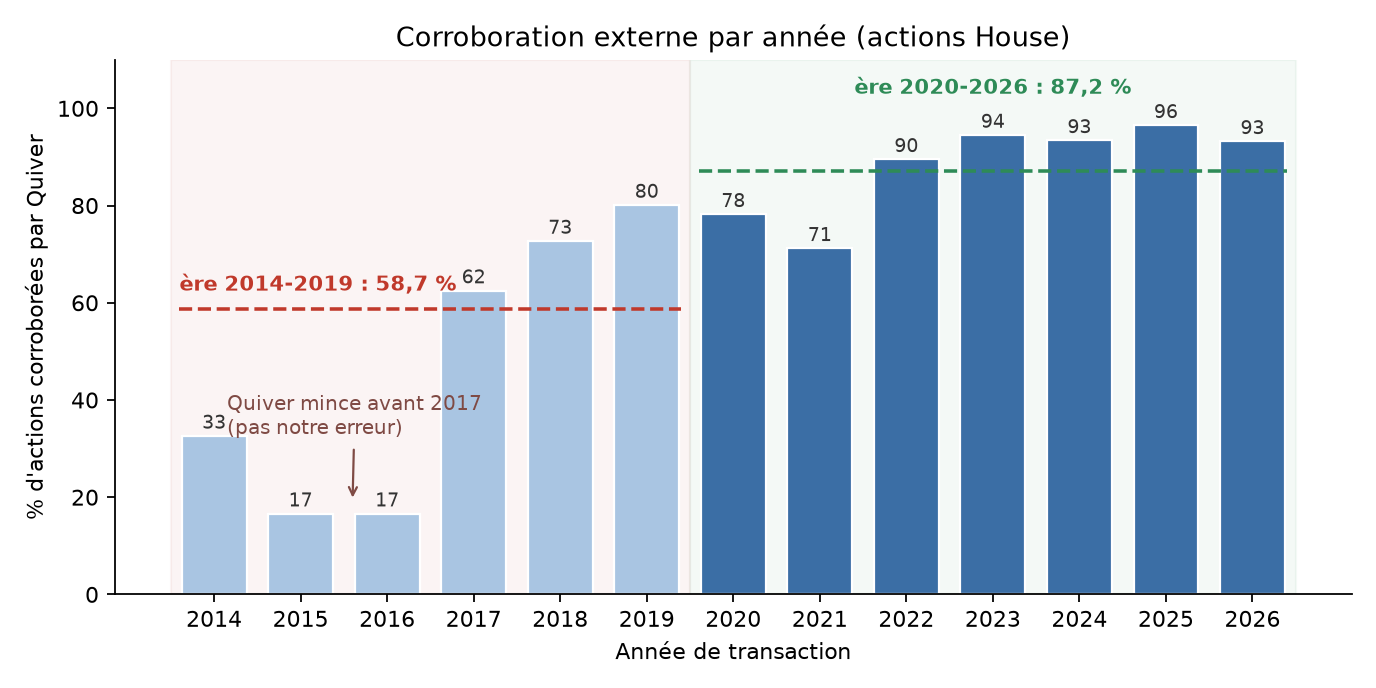
\includegraphics[width=\linewidth]{slides/fig_quiver_par_an.png}
    \end{column}
  \end{columns}
\end{frame}

% ── S18 · Quiver N2/N3 : les dates, qui a raison ? ── (RQ §6.3-6.5 ; audit §3 ; schema.py)
\begin{frame}{Validation (2/3) — les dates : qui a raison ?}
  \begin{columns}[T]
    \begin{column}{0.44\textwidth}
      {\footnotesize \textbf{niveau 2} — appariement \textbf{1-à-1} des dates,
       au sein de chaque (élu, ticker, sens) :}\\[1mm]
      \colorbox{black!6}{\parbox{0.97\linewidth}{\ttfamily\scriptsize
        Khanna, AAPL, Achat :\\
        NOUS\ \ \ : 08-jan · 13-fév · 01-juin\\
        QUIVER : 08-jan · 12-fév\\[0.8mm]
        \normalfont\scriptsize
        1.\ dates \textbf{identiques} retirées une à une (08-jan ↔ 08-jan)\\
        2.\ restes appariés au plus proche : 13-fév ↔ 12-fév = \emph{bruit} (≤10 j)\\
        3.\ 01-juin sans vis-à-vis → \textbf{nous-seul} (on est plus complet)}}\\[2mm]
      {\footnotesize → seuls \textbf{545 candidats} issus du \textbf{même dépôt}
       méritent l'œil → \textbf{arbitrage au PDF source} :}
    \end{column}
    \begin{column}{0.54\textwidth}
      {\small
      \begin{tabular}{@{}>{\raggedright\arraybackslash}p{0.34\linewidth}>{\raggedright\arraybackslash}p{0.29\linewidth}>{\raggedright\arraybackslash}p{0.30\linewidth}@{}}
        \toprule
        \textbf{le PDF montre…} & \textbf{exemple réel} & \textbf{traitement} \\
        \midrule
        {\scriptsize coquille du déposant, prouvable} & {\scriptsize\ttfamily 3031-04-30} & {\scriptsize corrigée → 2021} \\[0.6mm]
        {\scriptsize coquille littérale} & {\scriptsize le PTR imprime {\ttfamily 01/35/22}} & {\scriptsize\textcolor{okgreen}{\textbf{transcrite telle quelle}}} \\[0.6mm]
        {\scriptsize notre OCR s'est trompé} & {\scriptsize Khanna/COST {\ttfamily 09-31}} & {\scriptsize re-lue au PDF → {\ttfamily 08-16}} \\[0.6mm]
        {\scriptsize désaccord Quiver} & {\scriptsize McCaul/GOOGL $\Delta$11 j} & {\scriptsize arbitré au PDF ({\ttfamily doc 9113676})} \\
        \bottomrule
      \end{tabular}}\\[2.5mm]
      {\footnotesize \textbf{niveau 3} — sur les trades partagés, accord des
       \textbf{autres champs} :}\\[1mm]
      \badge{okgreen}{sens : 96,8\,\% Chambre · 99,9\,\% Sénat}\quad
      \badge{okgreen}{montant : 94,2\,\% · 99,8\,\%}
    \end{column}
  \end{columns}
\end{frame}

% ── S19 · Autres validations ── (AUDIT §3 ; RQ §1 ; crosscheck.py)
\begin{frame}{Validation (3/3) — les preuves indépendantes de Quiver}
  \centering
  \begin{minipage}[t]{0.32\textwidth}
    \carte{helec}{Univers officiel}{index du \emph{House Clerk} re-téléchargé :
      \textbf{100\,\%} des \textbf{8\,252 PTR} traités — parsés, OCRisés ou écartés
      par règle écrite}\\[2mm]
    \carte{okgreen}{senate-stock-watcher}{collecte indépendante, 6\,231 txns 2014-2020 :
      \textbf{100\,\%} retrouvées chez nous — on est un sur-ensemble strict}
  \end{minipage}\hfill
  \begin{minipage}[t]{0.32\textwidth}
    \carte{selec}{house-stock-watcher}{miroir indépendant 2018-2026 :
      \textbf{99,5\,\%} de ses lignes chez nous ; ses manques pré-2018 → tous traités}\\[2mm]
    \carte{warnorange}{Kadoa}{agrégateur tiers : comptes par déposant, triangulation
      automatisée (\co{test\_crosscheck}) — confirme les déposants où notre OCR
      est l'\textbf{unique source}}
  \end{minipage}\hfill
  \begin{minipage}[t]{0.32\textwidth}
    \carte{alertred}{Golden interne}{\textbf{368 tables figées} SHA-256, rejouées
      octet à octet à \textbf{zéro écart} ; invariants recomptés
      (digital + OCR = FINAL, identité 100\,\%)}\\[2mm]
    \colorbox{black!6}{\parbox[t][23mm][t]{\dimexpr\linewidth-8pt}{\vspace{1mm}
      {\footnotesize\textbf{le principe}}\\[0.8mm]{\scriptsize aucune source externe
      n'est \textbf{réinjectée} dans les tables — elles ne servent qu'à
      \textbf{mesurer} ce qu'on a}}}
  \end{minipage}
\end{frame}

% ═════════════ VI. LIVRABLE ═════════════
\section{Le livrable}

% ── S20 · Entonnoir ── (RQ §7)
\begin{frame}{Du corpus à la table de recherche : l'entonnoir}
  \begin{columns}[T]
    \begin{column}{0.60\textwidth}
      \centering
      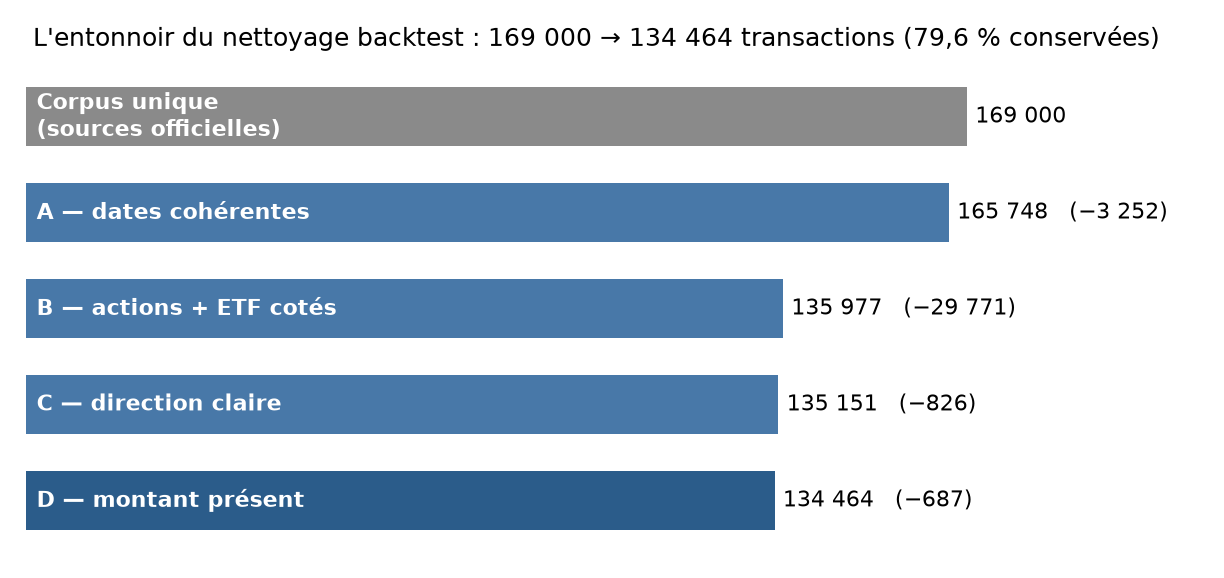
\includegraphics[width=\linewidth]{quality/entonnoir_backtest.png}
    \end{column}
    \begin{column}{0.38\textwidth}
      {\footnotesize\textbf{le principe} : on ne retire que l'\textbf{avéré
       inutilisable} pour un backtest (pas de date, pas de prix, pas de sens,
       pas de montant) —}\\[1mm]
      \badge{okgreen}{tout le doute est GARDÉ et FLAGUÉ}\\[3mm]
      {\footnotesize\textbf{les flags} (jamais retirés) :}\\[1mm]
      {\scriptsize
      · \co{flag\_late\_filing} — divulgué > 45 j : \textbf{12,2\,\%}\\[0.8mm]
      · \co{is\_delisted} — titre sorti de cote, typé (faillite/rachat) : 2,6\,\%\\[0.8mm]
      · \co{lot\_size} > 1 — lots multi-comptes réels : 8,8\,\%\\[0.8mm]
      · \co{flag\_price\_caution} — symbole recyclé : 0,4\,\%}
    \end{column}
  \end{columns}
\end{frame}

% ── S21 · Conclusion ── (RQ §7 ; CSV vérifié)
\begin{frame}{Le livrable — prêt pour la recherche}
  \centering
  \colorbox{helec}{\parbox{0.82\textwidth}{\footnotesize\color{white}\centering\vspace{1.5mm}
    \texttt{\small data/clean/transactions\_backtest\_2014\_2026.csv}\\[1.2mm]
    {\large\textbf{134\,464 lignes × 36 colonnes}}\\[0.8mm]
    372 membres · 57\,\% issu d'OCR · parti \& commissions \emph{point-in-time} ·
    traçable ligne à ligne (\co{doc\_id})\vspace{1.5mm}}}

  \vspace{5mm}
  \begin{columns}[T]
    \begin{column}{0.48\textwidth}
      {\footnotesize\textbf{Ce qu'on garantit}}\\[1mm]
      {\scriptsize
      ✓ complet : 100\,\% de l'univers officiel\\
      ✓ identifié : 100\,\% des lignes rattachées\\
      ✓ validé : Quiver + 3 sources indépendantes\\
      ✓ reproductible : golden octet à octet}
    \end{column}
    \begin{column}{0.48\textwidth}
      {\footnotesize\textbf{Limites assumées}}\\[1mm]
      {\scriptsize
      · 582 PTR manuscrits écartés (règle rejouable)\\
      · corroboration externe plus faible avant 2017\\
      · montants = fourchettes (milieu), pas des prix exacts}
    \end{column}
  \end{columns}
\end{frame}

% ═════════════ ANNEXES ═════════════
\appendix

% ═════════════ V. LA REFONTE V1 — la Chambre refaite, complétée et prouvée ═════════════
% Chiffres : 01_v1_house/cache/tables/*.csv + cache/MANIFEST.json (run post-B4, tout le papier OCRisé).
% Cette partie REMPLACE l'ancienne section V1 (pré-B4 : 37 validations, 56 002 txns, OCR annoncé
% comme une suite) et le PoC de cohérence sur 33 élus — la mesure définitive est ici.
\section{La refonte V1 — la Chambre refaite, complétée et prouvée}

\chapdivider{La refonte V1}{La Chambre, de bout en bout}{du site du Clerk au portefeuille daté de chaque élu — tout le papier lu, tout recoupé}

% ── V1-A · Le plan en 10 étapes + les deux compteurs ──
\begin{frame}{Le plan — dix étapes, dans l'ordre du réel}
  \centering
  {\footnotesize\setlength{\tabcolsep}{5pt}\renewcommand{\arraystretch}{1.1}
  \begin{tabular}{l l}
    \textbf{1 · Récupérer} & les 13 index annuels → 35\,377 dépôts recensés \\
    \textbf{2 · Router} & lisible ou scanné — le 1\ier{} chiffre du DocID le dit \\
    \textbf{3 · Identifier} & du nom imprimé à l'identifiant stable de l'élu \\
    \textbf{4 · Le cycle de vie} & qui entre, qui sort, qui reste \\
    \textbf{5 · Extraire} & le patrimoine (Schedule A) et les transactions (B) \\
    \textbf{6 · Le portefeuille d'entrée} & la photo de départ de chaque membre \\
    \textbf{7 · Les flux, dédupliqués} & les transactions de toutes les sources \\
    \textbf{8 · Vérifier} & entrée + achats doivent expliquer la sortie \\
    \textbf{9 · Reconstruire} & la série datée du patrimoine, membre par membre \\
    \textbf{10 · Rien d'oublié} & chaque dépôt a un traitement, la somme boucle \\
  \end{tabular}}\\[3mm]
  \colorbox{helec}{\parbox{0.92\textwidth}{\footnotesize\color{white}\centering
    \textbf{deux compteurs, jamais confondus} : on RECONSTRUIT le portefeuille de
    825 membres · on ne peut le VÉRIFIER de bout en bout que pour
    56 d'entre eux — et on sait exactement pourquoi}}\\[2.5mm]
  {\scriptsize\color{black!60} \textbf{périmètre de cette partie} : la \textbf{Chambre seule},
   \textbf{tous} les types de dépôts (P·O·H·T·A·C), \textbf{tout le papier OCRisé} — ses
   compteurs ne se comparent donc pas à ceux de la partie I (les PTR des deux chambres) ;
   règle d'or : \textbf{aucun ratio sans ses trois étiquettes} — unité × périmètre × fenêtre}
\end{frame}

% ── V1-B · La source s'efface ── (fig recalculée depuis cache/index*)
\begin{frame}{Découverte — la source primaire s'efface sous nos yeux}
  \centering
  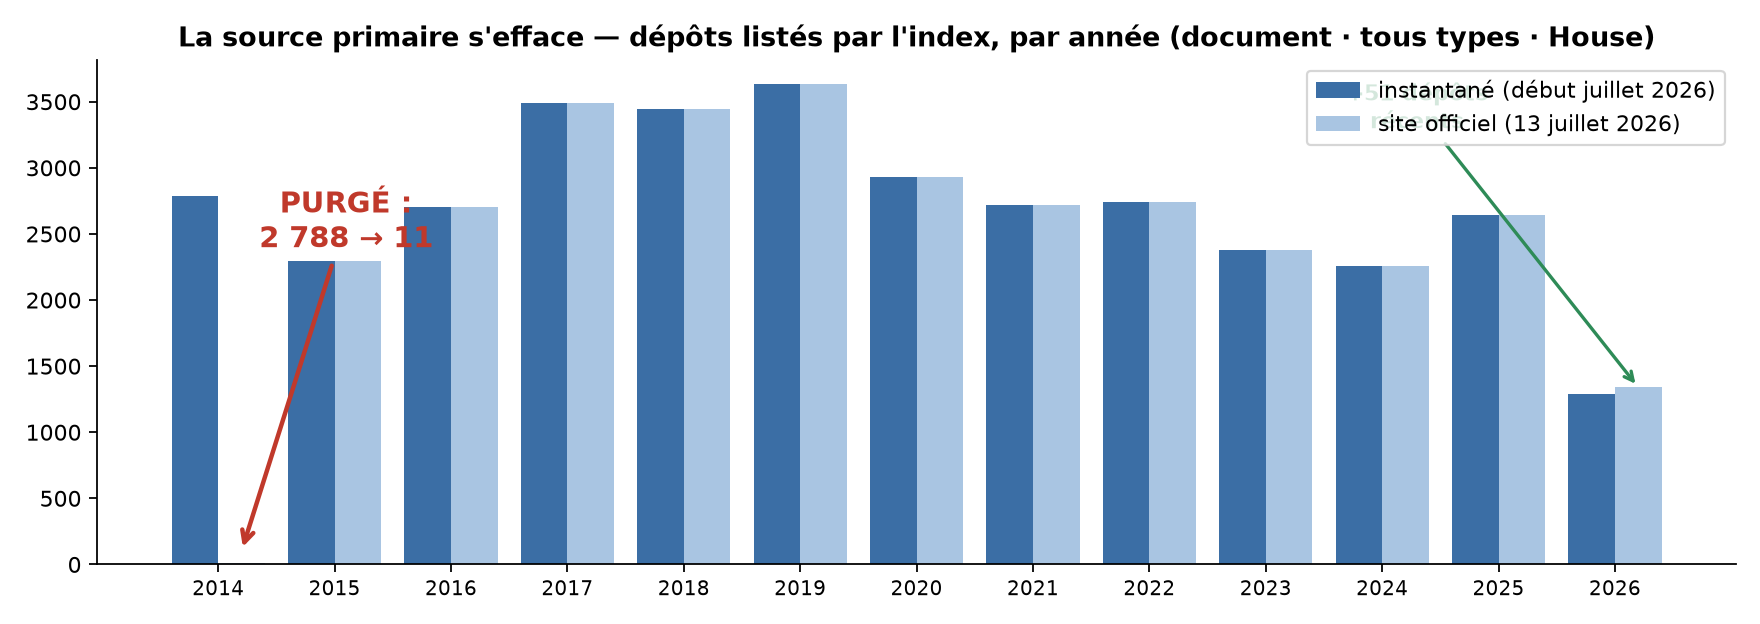
\includegraphics[height=0.40\textheight]{fig_v1_purge_index.png}\\[2.5mm]
  \tuile{helec}{35\,377}{dépôts recensés\\2014 → 2026}\hfill
  \tuile{alertred}{11}{dépôts de 2014 encore\\listés sur le site}\hfill
  \tuile{okgreen}{2\,784}{dépôts de 2014 dans\\NOTRE archive}\\[2.5mm]
  {\footnotesize le Clerk \textbf{purge} les index au-delà de $\sim$6 ans (la loi l'y autorise) :
   les PDF répondent encore, mais la \emph{liste de quoi demander} a disparu du site → le
   recensement = \textbf{site d'aujourd'hui $\cup$ notre archive}, chaque ligne tracée}
\end{frame}

% ── V1-C · Le routage prouvé ── (tables 02/03)
\begin{frame}{Le tri lisible/scanné n'est pas une hypothèse : c'est une mesure}
  \centering
  {\footnotesize le 1\ier{} chiffre du \co{DocID} \emph{annonce} la nature du document
   (\co{1/2/3/4} lisible · \co{7/8/9} scanné) — on ne le croit pas sur parole :
   on ouvre les \textbf{26\,088} PDF et on regarde s'ils contiennent réellement du texte}\\[3.5mm]
  {\normalsize\setlength{\tabcolsep}{12pt}\renewcommand{\arraystretch}{1.3}
  \begin{tabular}{l cc}
    \toprule
    & annoncé lisible & annoncé scanné \\
    \midrule
    contient du texte & \textcolor{okgreen}{\textbf{20\,821}} & \textcolor{alertred}{\textbf{0}} \\
    image seulement & \textcolor{alertred}{\textbf{0}} & \textcolor{okgreen}{\textbf{5\,267}} \\
    \bottomrule
  \end{tabular}}\\[4mm]
  \badge{okgreen}{zéro désaccord sur 26\,088 documents}\\[2mm]
  {\scriptsize\color{black!60} et chaque dépôt reçoit UN statut dans un registre (le « ledger »)
   dont la somme retombe exactement sur 35\,377 — rien ne se perd en silence}
\end{frame}

% ── V1-D · Les témoins ── (asserts littéraux du notebook, §7.2/§8.2/§8.3)
\begin{frame}{Cinq documents témoins, comptés à la main, verrouillent les parseurs}
  \centering
  {\footnotesize chaque gabarit est validé par un \textbf{assert littéral} sur un document
   ouvert et compté à la main — si un parseur régresse, le notebook \textbf{s'arrête}}\\[2.5mm]
  {\small
  \begin{tabular}{@{}llll@{}}
  \toprule
  témoin & gabarit & compté à la main & piège couvert \\
  \midrule
  \href{https://disclosures-clerk.house.gov/public_disc/ptr-pdfs/2014/20002235.pdf}{Yoder 2014} & PTR legacy & \textbf{5} txns & petites capitales, ticker en continuation \\
  \href{https://disclosures-clerk.house.gov/public_disc/ptr-pdfs/2020/20016985.pdf}{Allen 2020} & PTR moderne & \textbf{3} txns & montants coupés sur 2 lignes \\
  \href{https://disclosures-clerk.house.gov/public_disc/ptr-pdfs/2017/20006475.pdf}{Peters 2017} & PTR conjoint & \textbf{3} txns & palier « Spouse/DC over \$1M » \\
  \href{https://disclosures-clerk.house.gov/public_disc/financial-pdfs/2020/10042733.pdf}{Greene 2020 (H)} & Schedule A & \textbf{101} holdings & blocs « conteneur $\Rightarrow$ », IRA \\
  \href{https://disclosures-clerk.house.gov/public_disc/financial-pdfs/2015/10010857.pdf}{Pelosi 2015 (O)} & Schedule B FD & \textbf{5} txns & (partial) et borne sur ligne suivante \\
  \bottomrule
  \end{tabular}}\\[2.5mm]
  \badge{alertred}{401(k) lu « ticker K » : 567 faux — corrigé}\;
  \badge{warnorange}{montants exacts « \$955.10 » — captés}\;
  \badge{okgreen}{ETF exemptés de PTR par la loi — classés}
\end{frame}

% ── V1-E · Le procès de l'ancien ── (X1/X2, arbitrage marqueurs)
\begin{frame}{L'ancien pipeline au tribunal des documents}
  \centering
  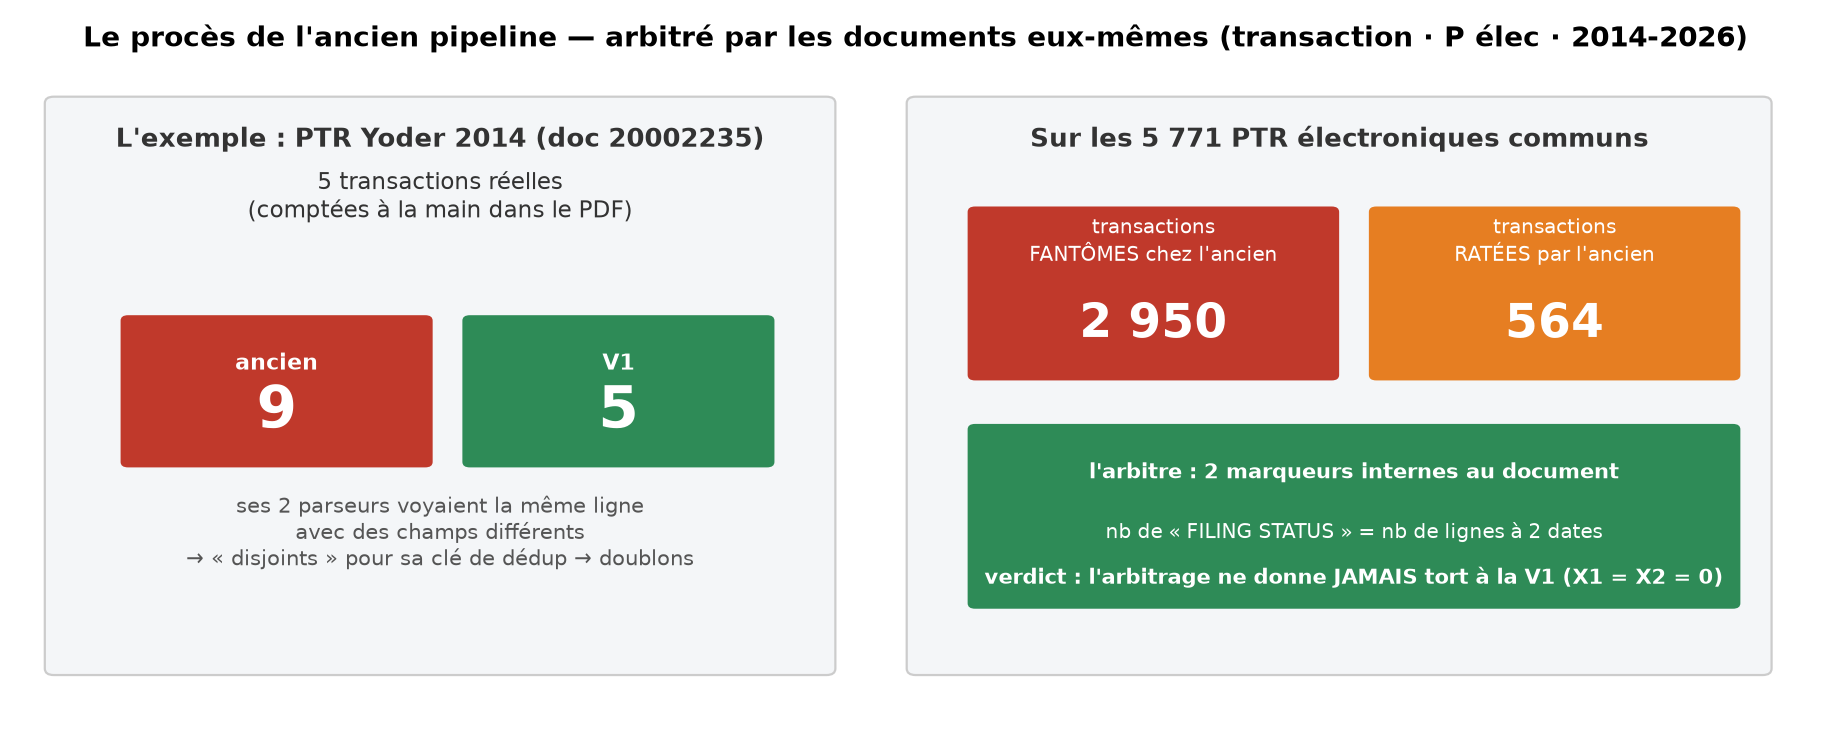
\includegraphics[width=0.96\textwidth]{fig_v1_fantomes.png}\\[1mm]
  {\scriptsize\color{black!60} chaque désaccord de compte est tranché par le document
   lui-même — pas par confiance envers l'un ou l'autre code}
\end{frame}

% ── V1-F · Qui dépose quoi ── (§15.2 du notebook, vérifié adversarialement)
\begin{frame}{Qui dépose quoi — la couverture réelle des entrées et des sorties}
  \centering
  {\footnotesize\setlength{\tabcolsep}{10pt}\renewcommand{\arraystretch}{1.25}
  \begin{tabular}{l l}
    \toprule
    \textbf{470 entrées} au Congrès & 82 \% ont déposé un \textbf{H} (déclaration d'entrée) \\
    (depuis 2014) & 16 \% un \textbf{C} à la place (la loi les dispense du H) \\
    & 2 \% ni l'un ni l'autre → \textbf{98 \% couverts} \\
    \midrule
    \textbf{463 sorties} définitives & 81 \% ont déposé un \textbf{T} (déclaration de sortie) \\
    & 86 sans T : partis au Sénat ou à l'exécutif \\
    & (dispensés), décès, départs trop récents \\
    \bottomrule
  \end{tabular}}\\[3.5mm]
  {\footnotesize presque chaque entrée a sa \textbf{photo de patrimoine} — mais une entrée
   sur cinq qui sort ne laisse \textbf{pas de photo de sortie}}\\[1.5mm]
  {\scriptsize\color{black!60} c'est cette disponibilité, et elle seule, qui décide
   de qui sera vérifiable de bout en bout}
\end{frame}

% ── V1-G · Le quadrant ── (table 14, colonne quadrant)
\begin{frame}{Les 900 membres de la fenêtre — qui peut-on tester de bout en bout ?}
  \centering
  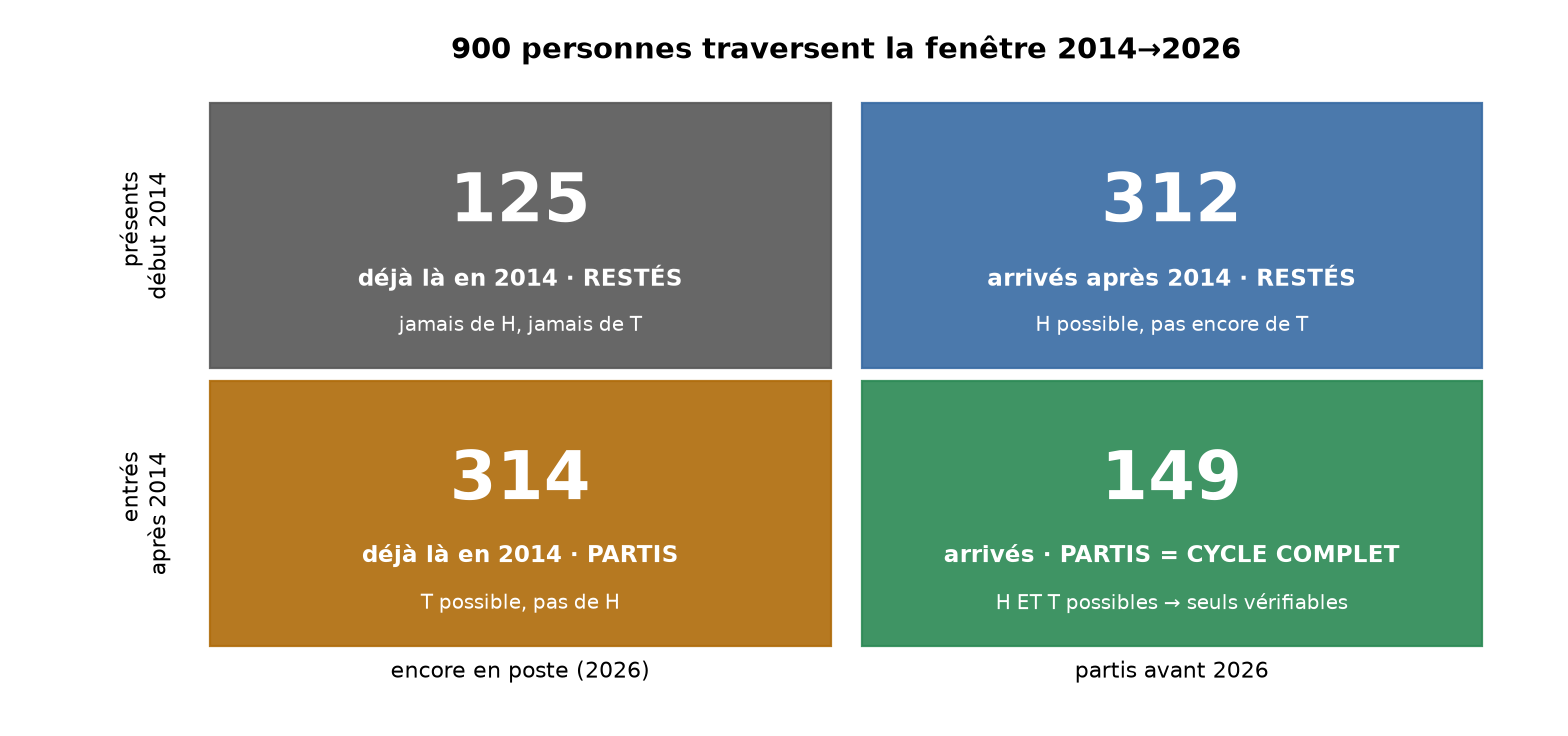
\includegraphics[width=0.66\textwidth]{fig_house_quadrant.png}\\[1.5mm]
  {\footnotesize les \textbf{439} déjà en poste en 2014 n'ont pas de photo d'entrée ·
   les \textbf{437} encore en poste n'ont pas de photo de sortie →
   \textbf{seuls les 149 entrés PUIS sortis} dans la fenêtre peuvent être vérifiés
   de bout en bout}\\[1mm]
  {\scriptsize\color{black!60} ce n'est pas un défaut de collecte : c'est la structure
   même de la fenêtre 2014-2026}
\end{frame}

% ── V1-H · Les 4 canaux ── (tables 04/05/07/08/09 ; post-B4 : tout le papier lu)
\begin{frame}{Quatre canaux d'extraction — l'électronique d'abord, l'OCR pour tout le reste}
  \centering
  \tuile{dataC}{198\,615}{photos de patrimoine\\électroniques}\hfill
  \tuile{helec}{56\,002}{transactions P\\électroniques}\hfill
  \tuile{helec}{110\,147}{transactions des\\annuels (électroniques)}\hfill
  \tuile{hocr}{449\,350}{lignes lues par OCR\\(tout le scanné)}\\[4mm]
  {\footnotesize \badge{okgreen}{rien de lisible ne part inutilement en OCR — et zéro
   document scanné n'a été laissé de côté}}\\[2.5mm]
  {\scriptsize\color{black!60} l'OCR livre 105\,074 transactions P + 188\,970 photos de
   patrimoine + 155\,306 transactions d'annuels — c'est tout le patrimoine papier de la
   Chambre, lu pour la première fois}
\end{frame}

% ── V1-I · Ce que l'extraction livre ── (MANIFEST ; 28 j = médiane vérifiée)
\begin{frame}{Ce que l'extraction livre}
  \centering
  \tuile{okgreen}{161\,076}{transactions datées\\= LE SIGNAL}\hfill
  \tuile{helec}{28 j}{délai médian\\trade → publication}\hfill
  \tuile{dataC}{387\,585}{photos de patrimoine\\(toutes sources)}\\[4mm]
  {\footnotesize le signal, c'est les \textbf{P} : les seules transactions connues assez vite
   pour être tradées. Tout le reste — photos de patrimoine et transactions des annuels —
   sert à \textbf{reconstruire et vérifier} les portefeuilles.}
\end{frame}

% ── V1-J · La photo de départ ── (table 15 ; 3 garde-fous sur la porte C)
\begin{frame}{La photo de départ de chaque membre}
  \centering
  \tuile{okgreen}{252}{membres ancrés\\par leur H}\hfill
  \tuile{dataC}{32}{ancrés par leur C\\(dispensés de H)}\hfill
  \tuile{helec}{284}{= portefeuilles\\d'entrée datés}\hfill
  \tuile{grisC}{616}{sans photo d'entrée\\(déjà en poste en 2014…)}\\[4mm]
  {\footnotesize un \textbf{C} n'est accepté comme photo de départ que sous
   \textbf{trois garde-fous} : électronique · au moins une action cotée · déposé moins
   d'un an avant la prise de poste (le C de campagne d'un élu déjà en place ne compte pas)}\\[2mm]
  {\scriptsize\color{black!60} sans H ni C, la reconstruction s'ancre sur le premier
   rapport annuel — plus tardif, donc série partielle}
\end{frame}

% ── V1-K · Dédup à l'assemblage + gain net des annuels ── (§10 du notebook ; table 16)
\begin{frame}{Les transactions ne vivent pas que dans les P — et ce que ça rapporte}
  \centering
  {\footnotesize les annuels (O), les amendements (A) et les sorties (T) déclarent AUSSI
   des transactions — souvent les mêmes, re-déclarées}\\[3mm]
  \resizebox{0.86\textwidth}{!}{%
  \begin{tikzpicture}[node distance=9mm]
    \node[step=helec, text width=3.2cm, minimum height=1.5cm, font=\footnotesize] (a)
      {\textbf{189\,117} lignes\\{\scriptsize toutes sources confondues}};
    \node[step=dataC, text width=3.4cm, minimum height=1.5cm, font=\footnotesize, right=of a] (b)
      {\textbf{−\,22\,968} doublons\\{\scriptsize le même trade re-déclaré\\(annuel, amendement…)}};
    \node[step=okgreen, text width=3.2cm, minimum height=1.5cm, font=\footnotesize, right=of b] (c)
      {\textbf{166\,149} uniques\\{\scriptsize chaque trade compté\\UNE fois}};
    \draw[arr] (a) -- (b); \draw[arr] (b) -- (c);
  \end{tikzpicture}}\\[3.5mm]
  \tuile{okgreen}{26\,115}{trades jamais vus\\dans un P}\hfill
  \tuile{dataC}{22\,216}{via les\\annuels}\hfill
  \tuile{dataC}{3\,899}{via sorties et\\amendements}\hfill
  \tuile{grisC}{374 j}{délai médian\\trade → publication}\\[2.5mm]
  {\footnotesize ces trades comblent des trous du portefeuille (des élus oublient leur P mais
   l'inscrivent à l'annuel) — on les découvre \textbf{un an trop tard} : ils nourrissent le
   patrimoine, \textbf{jamais le signal}}
\end{frame}

% ── V1-L · Le test de cohérence ──
\begin{frame}{Le test de cohérence — la chronologie d'un mandat doit se recouper}
  \centering
  {\footnotesize chaque position détenue à la SORTIE doit s'expliquer : soit elle était là
   à l'ENTRÉE, soit elle a été ACHETÉE entre les deux}\\[4mm]
  \resizebox{0.90\textwidth}{!}{%
  \begin{tikzpicture}[node distance=8mm]
    \node[step=okgreen, text width=3.0cm, minimum height=1.6cm, font=\footnotesize] (h)
      {\textbf{photo d'ENTRÉE}\\{\scriptsize ce qu'il possède\\en arrivant}};
    \node[step=helec, text width=3.2cm, minimum height=1.6cm, font=\footnotesize, right=of h] (p)
      {\textbf{+ les ACHATS}\\{\scriptsize toutes les transactions\\du mandat}};
    \node[step=dataC, text width=3.2cm, minimum height=1.6cm, font=\footnotesize, right=of p] (t)
      {\textbf{doit couvrir la SORTIE}\\{\scriptsize chaque position,\\une par une}};
    \draw[arr] (h) -- (p); \draw[arr] (p) -- (t);
  \end{tikzpicture}}\\[4mm]
  {\footnotesize quatre déclarations \textbf{indépendantes} du même portefeuille (entrée,
   transactions, annuels, sortie) : \textbf{si la collecte était trouée, ça se verrait ici}}\\[1.5mm]
  {\scriptsize\color{black!60} le croisement n'est possible que parce que chaque dépôt est
   rattaché à l'identifiant officiel de l'élu : 99,9 \% des transactions,
   99,2 \% des entrées et des sorties}
\end{frame}

% ── V1-M · La cohorte testable ──
\begin{frame}{Sur qui peut-on faire ce test ?}
  \centering
  \resizebox{0.88\textwidth}{!}{%
  \begin{tikzpicture}[node distance=9mm]
    \node[step=grisC, text width=3.2cm, minimum height=1.6cm, font=\footnotesize] (a)
      {\textbf{149} cycles complets\\{\scriptsize entrés PUIS sortis\\dans la fenêtre}};
    \node[step=dataC, text width=3.2cm, minimum height=1.6cm, font=\footnotesize, right=of a] (b)
      {\textbf{106} avec les\\deux photos déposées\\{\scriptsize entrée ET sortie}};
    \node[step=okgreen, text width=3.4cm, minimum height=1.6cm, font=\footnotesize, right=of b] (c)
      {\textbf{56} testables\\{\scriptsize des actions cotées\\des deux côtés}};
    \draw[arr] (a) -- (b); \draw[arr] (b) -- (c);
  \end{tikzpicture}}\\[4mm]
  {\footnotesize la moitié des membres à double photo ne détient \textbf{aucune action cotée}
   (fonds, immobilier, comptes gérés) — on ne peut pas suivre ce qui n'a pas de cours de
   bourse : c'est la nature du patrimoine, pas un défaut de collecte}
\end{frame}

% ── V1-N · Le résultat ── (MANIFEST : 78,7 / 87,8 / 3,3 ; cohorte élargie 87,1)
\begin{frame}{Le résultat — les portefeuilles se recoupent}
  \centering
  \tuile{helec}{78,7 \%}{expliqué par les\\transactions P seules}\hfill
  \tuile{okgreen}{87,8 \%}{avec TOUTES les\\déclarations}\hfill
  \tuile{alertred}{3,3 \%}{vraiment\\inexpliqué}\\[4mm]
  {\footnotesize l'écart entre les deux premiers chiffres, c'est surtout du
   \textbf{non-dépôt documenté} : l'élu a déclaré l'achat dans son annuel, jamais dans un P —
   quelques habitués concentrent l'essentiel}\\[2.5mm]
  {\scriptsize\color{black!60} deux limites assumées : les montants sont des
   \textbf{fourchettes sans quantités} (on vérifie la présence d'un titre, pas un solde
   comptable) · les blind trusts ne créent pas de faux trous — le portefeuille y devient
   invisible, il ne fuit pas · la cohorte élargie au papier confirme (87,1 \%)}
\end{frame}

% ── V1-O · Le moteur ── (tables 12/13)
\begin{frame}{Le moteur — photo, flux, recalage}
  \centering
  \resizebox{0.90\textwidth}{!}{%
  \begin{tikzpicture}[node distance=8mm]
    \node[step=okgreen, text width=3.0cm, minimum height=1.6cm, font=\footnotesize] (a)
      {\textbf{photo d'ancrage}\\{\scriptsize la photo d'entrée,\\ou la 1\iere{} disponible}};
    \node[step=helec, text width=3.2cm, minimum height=1.6cm, font=\footnotesize, right=of a] (b)
      {\textbf{+ flux datés}\\{\scriptsize achats et ventes,\\appliqués jour par jour}};
    \node[step=dataC, text width=3.4cm, minimum height=1.6cm, font=\footnotesize, right=of b] (c)
      {\textbf{recalage}\\{\scriptsize à chaque nouvelle photo,\\le document fait foi}};
    \draw[arr] (a) -- (b); \draw[arr] (b) -- (c);
    \draw[arr, bend right=25] (c.south) to (b.south);
  \end{tikzpicture}}\\[4mm]
  \tuile{helec}{825}{membres avec un\\portefeuille daté}\hfill
  \tuile{dataC}{6\,049}{photos de patrimoine\\dans leurs séries}\hfill
  \tuile{okgreen}{66,7 \%}{des positions confirmées\\d'une photo à l'autre}\\[2.5mm]
  {\scriptsize\color{black!60} en positions et en fourchettes de valeur — jamais en
   quantités : la loi ne les publie pas}
\end{frame}

% ── V1-P · Le registre ── (table 14)
\begin{frame}{Un statut explicite pour chacun des 900 membres}
  \centering
  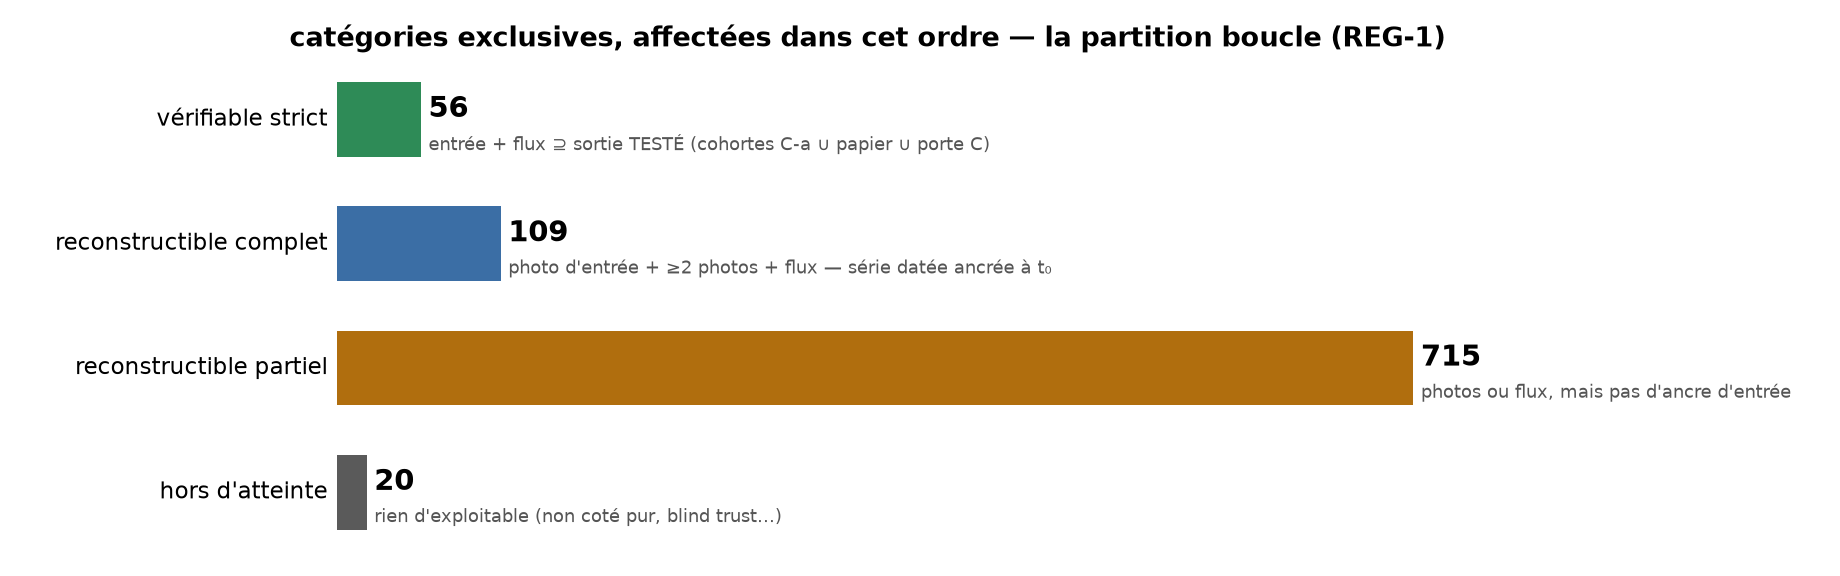
\includegraphics[width=0.86\textwidth]{fig_house_registre.png}\\[2mm]
  {\footnotesize « le portefeuille de chaque membre » se dit honnêtement : qui est
   \textbf{vérifié}, qui est \textbf{reconstruit avec son point de départ}, qui est
   \textbf{partiel}, qui est \textbf{hors d'atteinte} — et pourquoi, membre par membre}
\end{frame}

% ── V1-Q · Les deux compteurs ── (MANIFEST + table 18)
\begin{frame}{Les deux compteurs — reconstruire n'est pas vérifier}
  \centering
  \tuile{helec}{825}{portefeuilles\\RECONSTRUITS}\hfill
  \tuile{okgreen}{56}{portefeuilles VÉRIFIÉS\\de bout en bout}\\[4mm]
  {\footnotesize ces deux nombres ne s'additionnent ni ne se comparent : pour
   $\approx$ 9 membres sur 10, on reconstruit la série \textbf{sans pouvoir la vérifier}
   entrée → sortie (pas de cycle complet dans la fenêtre, ou pas d'actions cotées)}\\[2.5mm]
  {\scriptsize\color{black!60} et ce qui ne colle pas entre deux photos est \textbf{publié et
   décomposé}, pas caché — l'essentiel vient des libellés d'actifs qui changent d'écriture
   d'une année à l'autre (la suite naturelle : un appariement tolérant aux variations de nom)}
\end{frame}

% ── V1-R · Rien d'oublié + les contrôles ── (table 10 ; MANIFEST : 75 validations, 0 rouge)
\begin{frame}{Rien d'oublié — la somme boucle, et tout est re-jouable}
  \centering
  
\includegraphics[width=0.58\textwidth]{fig_house_compta.png}\\[2mm]
  \tuile{okgreen}{75}{contrôles automatiques\\dans le notebook}\hfill
  \tuile{helec}{0}{contrôle\\en échec}\hfill
  \tuile{dataC}{18}{tables versionnées\\(chaque chiffre traçable)}\\[2.5mm]
  {\footnotesize \badge{okgreen}{la somme des statuts retombe exactement sur 35\,377}\;
   \badge{okgreen}{zéro document scanné laissé de côté}\;
   \badgel{grisC!25}{\textcolor{grisC}{\textbf{10 exclus : des PDF morts côté site, tracés un par un}}}}\\[1.5mm]
  {\scriptsize\color{black!60} chaque affirmation de cette partie sort d'un contrôle du
   notebook : un chiffre faux ferait échouer l'exécution}
\end{frame}

% ── V1-S · Verdict ──
\begin{frame}{Ce que la refonte V1 prouve — et la suite}
  \centering
  {\footnotesize
  \badge{helec}{1. la source est exhaustive et ARCHIVÉE — c'est le site qui efface, pas nous}\\[2mm]
  \badge{helec}{2. le tri lisible/scanné est MESURÉ — et tout le scanné a été lu}\\[2mm]
  \badge{helec}{3. les portefeuilles SE RECOUPENT — 87,8 \% expliqué, 3,3 \% d'inexpliqué résiduel}}\\[5mm]
  \tuile{okgreen}{161\,076}{transactions datées\\= le signal, complet}\hfill
  \tuile{dataC}{825}{portefeuilles\\reconstruits et datés}\hfill
  \tuile{helec}{56}{vérifiés\\de bout en bout}\\[4mm]
  {\scriptsize\color{black!60} la suite : le Sénat sur le même plan · l'appariement tolérant
   des noms d'actifs · brancher le portefeuille d'entrée dans le moteur de stratégie}
\end{frame}

% ═════════════ VI. LA STRATÉGIE 05b — chiffres : 05b_Portefeuille_Membre_MathSpec.ipynb ═════════════
% (Parties I §0-§10 et II §11-§12 ; la Partie III « autopsie » viendra plus tard.)
% Toutes les figures fig_05b_* sont recalculées par le MÊME moteur que le notebook,
% avec contrôles bloquants sur chaque scalaire imprimé (118 029 / 266 / 223 / 20-12 / t 0,94 / etc.)

% ── Séparateur · PARTIE II ──
\partdivider{helec}{PARTIE II}{Le backtest}{reconstruire les portefeuilles, copier les meilleurs, mesurer l'alpha face au SPY}

\section{S3 — Le portefeuille des élus : le copy-trading bat-il le marché ?}

% ══ Carte chronologique (remplace l'ancien « pont ») : les 2 stratégies, un même verdict ══
\begin{frame}{Le plan : deux stratégies, un même verdict}
  \centering
  {\footnotesize la donnée est prête — \textbf{copier les élus rapporte-t-il de l'alpha ?}}\\[6mm]
  \resizebox{\textwidth}{!}{%
  \begin{tikzpicture}[node distance=9mm]
    \node[step=helec, text width=3.0cm] (a) {\textbf{A · Construire}\\[0.6mm]1 élu = 1 portefeuille en parts, valorisé jour par jour};
    \node[step=helec, text width=3.4cm, right=of a] (b) {\textbf{B · Stratégie 1}\\[0.6mm]classer par l'IR \& l'alpha, copier le top-$K$};
    \node[step=selec, text width=3.4cm, right=of b] (c) {\textbf{C · Stratégie 2}\\[0.6mm]changer de règle : classer au Sharpe brut};
    \node[step=alertred, text width=2.4cm, right=of c] (d) {\textbf{D · Verdict}\\[0.6mm]$\beta$ de style,\\$\alpha \approx 0$};
    \draw[arr] (a) -- (b);
    \draw[arr] (b) -- (c) node[midway, above, font=\scriptsize\bfseries, text=alertred] {pas d'$\alpha$};
    \draw[arr] (c) -- (d) node[midway, above, font=\scriptsize\bfseries, text=alertred] {pas d'$\alpha$};
  \end{tikzpicture}}\\[6mm]
  {\scriptsize\color{black!60} le même moteur de portefeuille sert les deux stratégies — seule la \textbf{règle de sélection} change}
\end{frame}

% ═════════════ CHAPITRE A ═════════════
\chapdivider{Chapitre A}{Construire le portefeuille}{un flux de trades $\rightarrow$ une NAV valorisée jour par jour}

% ── A1 · Reconstruction en parts (données repliées en 1 ligne d'entrée) ──
\begin{frame}{Le moteur — un flux de trades devient un portefeuille en parts}
  \begin{columns}[T]
    \begin{column}{0.47\textwidth}
      {\footnotesize entrée : \textbf{118\,029} trades exploitables (sur 134\,429 ; prix Yahoo blindés) ;
       montant = milieu de fourchette STOCK Act ; $\tau$ = 1\iere{} séance cotée $\geq$ date du trade}\\[2mm]
      {\color{helec}\footnotesize\textbf{acheter → recevoir des parts}}
      $$q=\frac{\text{montant}}{P_i(\tau)}$$
      {\color{alertred}\footnotesize\textbf{vendre → en rendre (short interdit)}}
      $$q^{-}=\min\!\Big(\frac{\text{montant}}{P_i(\tau)},\ n_i\Big)$$
      {\color{grisC}\footnotesize\textbf{cumuler, puis valoriser}}
      $$n_i(t)=\!\!\sum_{\text{trades}\,\le\,t}\!\!\pm q \qquad V(t)=\sum_i n_i(t)\,P_i(t)$$
    \end{column}
    \begin{column}{0.51\textwidth}\centering
      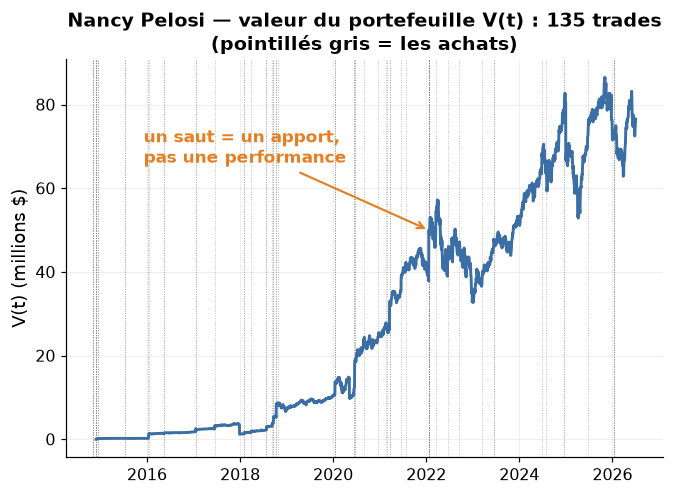
\includegraphics[width=\linewidth]{fig_05b_pelosi_valeur.png}\\[1mm]
      {\scriptsize\color{black!60} $V(t)$ mélange apports et performance
       → il faut un rendement qui les sépare}
    \end{column}
  \end{columns}
\end{frame}

% ── A2 · Rendement time-weighted ──
\begin{frame}{Le rendement time-weighted : un apport n'est jamais une performance}
  \centering
  {\footnotesize on valorise \textbf{les parts d'hier} aux prix d'aujourd'hui — l'argent frais n'entre qu'au lendemain\;
   (winsor ±50 \%/jour)}\\[1mm]
  $r_P(t)=\dfrac{\sum_i n_i(t{-}1)\,P_i(t)}{\sum_i n_i(t{-}1)\,P_i(t{-}1)}-1
   \qquad\quad \mathrm{NAV}(t)=\prod_{s\le t}\bigl(1+r_P(s)\bigr)$\\[2mm]
  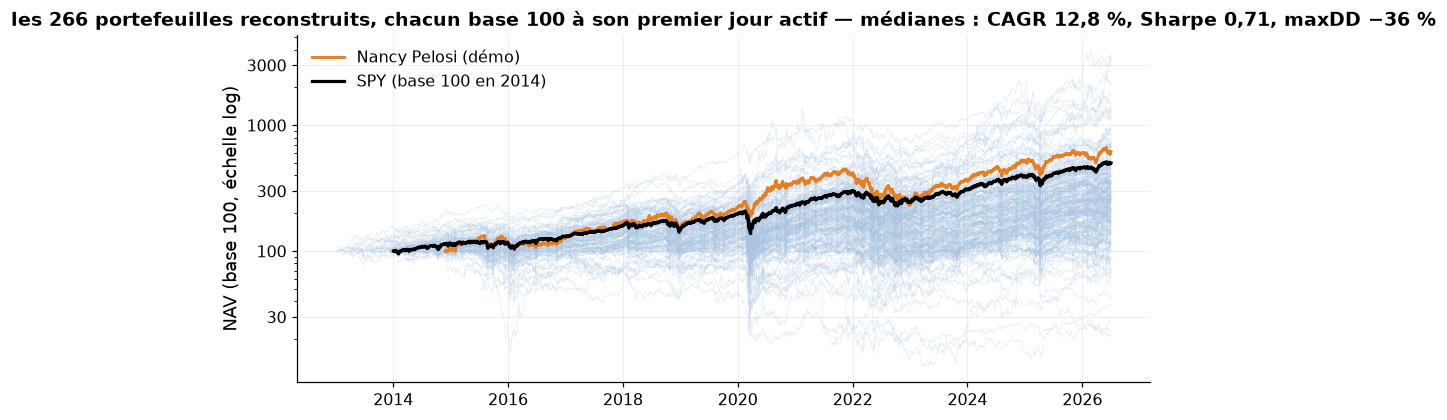
\includegraphics[height=0.52\textheight]{fig_05b_spaghetti_nav.png}\\[0.5mm]
  {\scriptsize\color{black!60} 266 portefeuilles reconstruits — médianes : CAGR 12,8 \%, Sharpe 0,71}
\end{frame}

% ═════════════ CHAPITRE B — STRATÉGIE 1 ═════════════
\chapdivider{Chapitre B · Stratégie 1}{Repérer et copier les « talents »}{qui bat le SPY ? on classe par l'IR et l'alpha, on copie le top-$K$}

% ── B1 · Éligibilité ──
\begin{frame}{La porte d'entrée : 223 membres sur 266 sont jugeables}
  \centering
  {\footnotesize éligible $\iff$ $n_{\text{trades}} \geq 10$ \textbf{et} $n_{\text{jours}} \geq 126$ ($\sim$ 6 mois de bourse)}\\[2mm]
  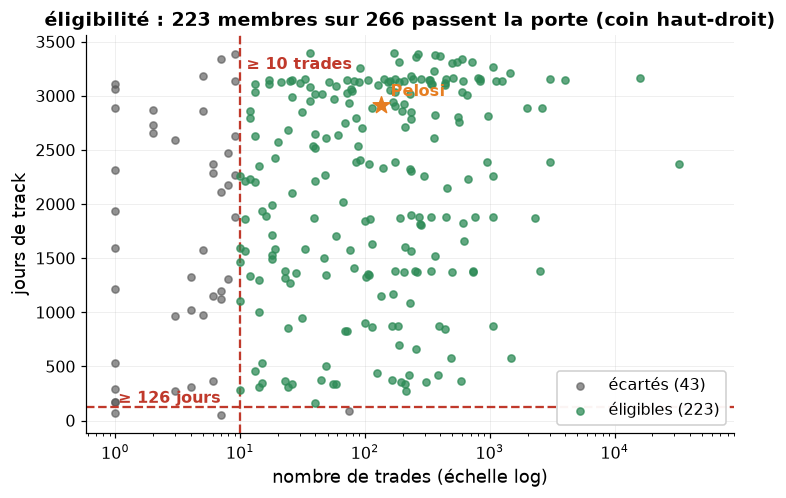
\includegraphics[height=0.62\textheight]{fig_05b_eligibilite.png}\\[1.5mm]
  {\scriptsize\color{black!60} sous les seuils : trop court pour distinguer chance et talent —
   \textbf{exclus du jugement}, pas des données}
\end{frame}

% ── B2 · Les deux mètres : IR & alpha ──
\begin{frame}{Deux mètres pour « battre le SPY » : l'écart brut (IR) ou l'alpha ajusté du $\beta$}
  \begin{columns}[T]
    \begin{column}{0.54\textwidth}
      {\color{helec}\footnotesize\textbf{Le mètre IR — suppose $\beta = 1$}\quad
       {\color{black!60}($x$ = excès quotidien sur le SPY)}}
      $$x(t)=r_P(t)-r_{\mathrm{SPY}}(t)\qquad \mathrm{IR}=\frac{\overline{x}}{\sigma(x)}\sqrt{252}$$
      {\color{selec}\footnotesize\textbf{Le mètre appraisal — estime $\beta$, le retire}}
      $$r_P(t)=\alpha+\beta\,r_{\mathrm{SPY}}(t)+\varepsilon(t)$$
      $$\mathrm{appr}=\frac{\alpha}{\sigma(\varepsilon)}\sqrt{252}\qquad
        \alpha_{\mathrm{ann}}=(1+\alpha)^{252}-1$$
      \centering
      \badgel{hocr}{$\beta=1 \ \Rightarrow\ $ appraisal $=$ IR}\\[1mm]
      {\scriptsize test unilatéral, seuil $t>1{,}645$}
    \end{column}
    \begin{column}{0.44\textwidth}\centering
      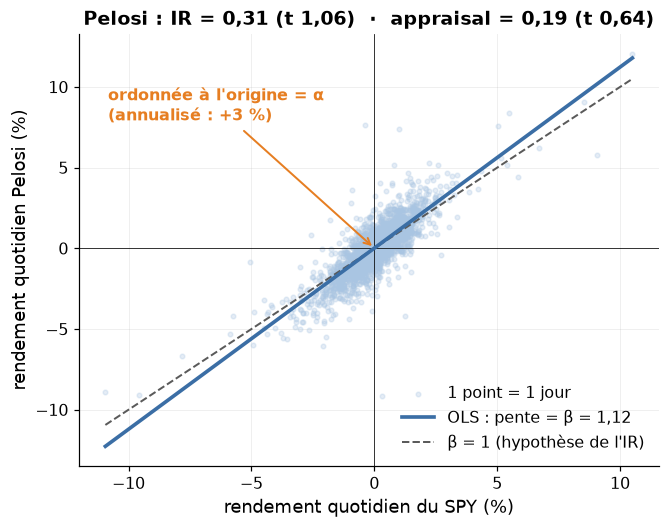
\includegraphics[width=0.93\linewidth]{fig_05b_regression_demo.png}\\[0.5mm]
      {\scriptsize\color{black!60} la pente absorbe le marché ;
       l'ordonnée à l'origine, c'est le talent}
    \end{column}
  \end{columns}
\end{frame}

% ── B3 · La mesure ne trouve presque rien (20 → 12 ≈ 11) ──
\begin{frame}{La mesure ne trouve presque rien : 20 « gagnants », 12 après le $\beta$, 11 par hasard}
  \centering
  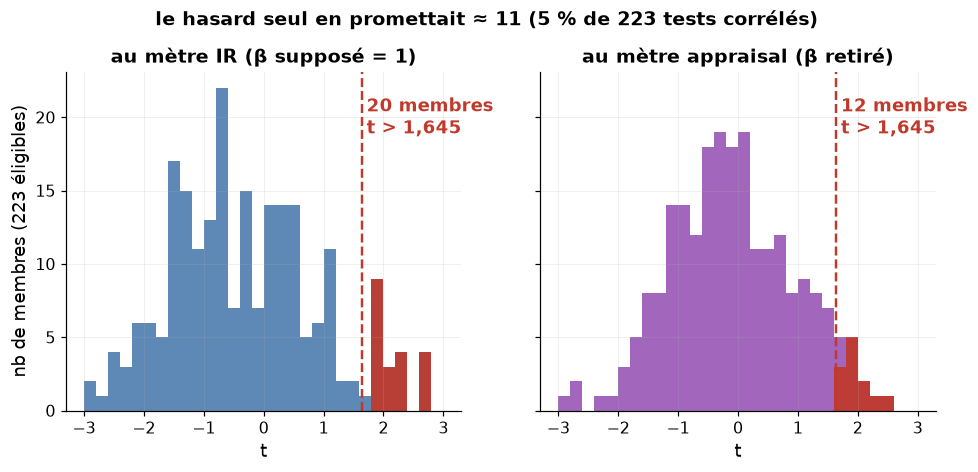
\includegraphics[height=0.58\textheight]{fig_05b_hist_t.png}\\[2mm]
  {\footnotesize \textbf{20} membres battent le SPY à l'IR, \textbf{12} seulement une fois le $\beta$ retiré (appraisal) —
   pour \textbf{$\approx$11} attendus par pur hasard (5 \% de 223)}\\[0.6mm]
  {\scriptsize\color{black!60} ajusté du $\beta$, le surnombre de « talents » retombe au niveau du bruit
   (détail en annexe)}
\end{frame}

% ── B4 · On copie le top-K en parts (walk-forward + parts, fusionnés) ──
\begin{frame}{On copie le top-$K$ en parts — sans jamais regarder le futur}
  \begin{columns}[T]
    \begin{column}{0.51\textwidth}
      {\footnotesize \textbf{walk-forward} : à chaque coupe fin $Y$, on classe les éligibles
       ($t_{\text{crit}}>1{,}645$) et on tient le top-$K$ toute l'année $Y{+}1$ —
       \textbf{aucune info postérieure à la coupe}}\\[2.5mm]
      {\footnotesize \textbf{en parts} : chaque élu $k$ = un fonds de prix $\mathrm{NAV}^k$ ;
       à la coupe on redéploie le capital $W$, puis buy-and-hold}
      $$\mathrm{nbr}^k_Y=\frac{w_k\,W}{\mathrm{NAV}^k(t^R_Y)},\qquad w_k=\tfrac{1}{|S_Y|}$$
      $$\mathrm{NAV}(t)=\!\!\sum_{k\in S_Y}\!\!\mathrm{nbr}^k_Y\,\mathrm{NAV}^k(t)$$
      $$r_{\text{strat}}(t)=\frac{\mathrm{NAV}(t)}{\mathrm{NAV}(t{-}1)}-1$$
      {\scriptsize\color{black!60} autofinancé (NAV continue) ; 11 coupes, fin 2015 → fin 2025
       — mécanique détaillée en annexe}
    \end{column}
    \begin{column}{0.47\textwidth}\centering
      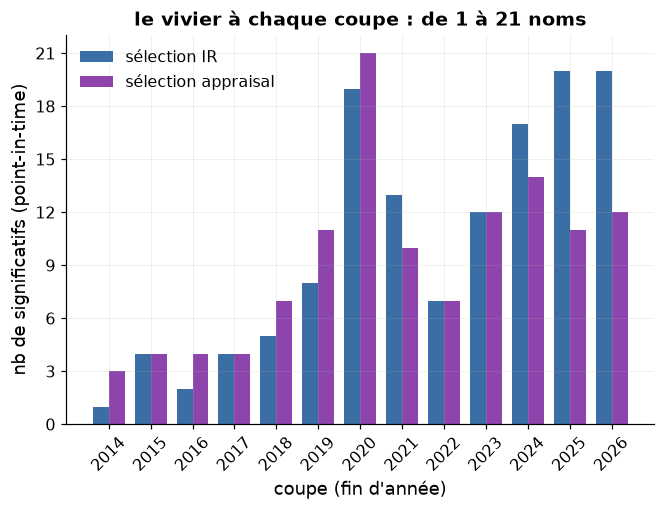
\includegraphics[width=\linewidth]{fig_05b_nsig_par_an.png}\\[1mm]
      {\scriptsize\color{black!60} le vivier à chaque coupe :
       de quoi alimenter un top-$K$ chaque année}
    \end{column}
  \end{columns}
\end{frame}

% ── B5 · Résultat top-4 ──
\begin{frame}{Top-4 : +3,1 \%/an d'excès… mais $t = 0{,}94$, et l'alpha dit zéro}
  \centering
  {\footnotesize 1 année civile = 1 observation :
   $x_Y=\prod_{t\in Y}(1+r_{\text{strat}})-\prod_{t\in Y}(1+r_{\mathrm{SPY}})$ ;\;
   $t=\overline{x}/\sigma(x)\cdot\sqrt{11}$ ; seuil $t_{10}\approx 1{,}81$}\\[1mm]
  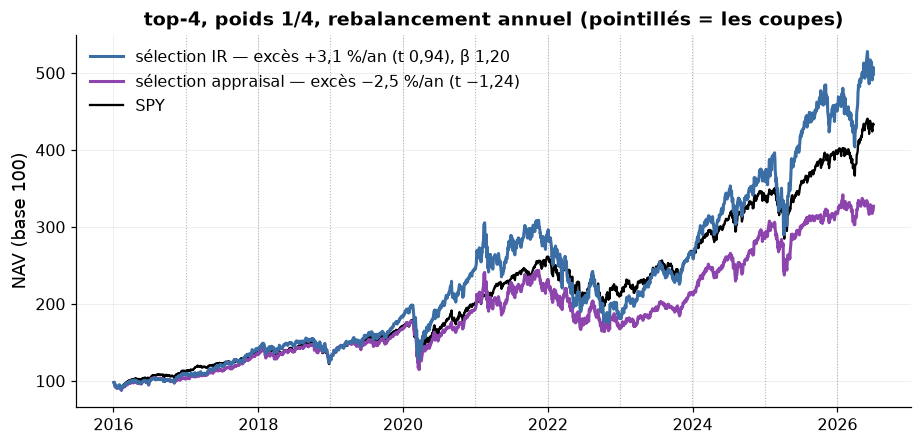
\includegraphics[height=0.47\textheight]{fig_05b_nav_top4.png}\\[2mm]
  \tuile{helec}{+3,1 \%/an}{excès brut\\7/11 années}\hfill
  \tuile{alertred}{t = 0,94}{$<$ 1,81 —\\indiscernable du hasard}\hfill
  \tuile{warnorange}{$\beta$ = 1,20}{l'excès = du style,\\pas du talent}\hfill
  \tuile{grisC}{$\alpha \approx 0$}{$t_{\text{appr}}$ −0,13 ;\\appraisal −2,5 \%/an}
\end{frame}

% ── B6 · On pousse : optimiser K et la cadence ──
\begin{frame}{On pousse : optimiser le nombre $K$, accélérer la cadence}
  \centering
  {\footnotesize le top-4 ne passe pas → on laisse $K$ \textbf{s'ajuster chaque année}
   ($K^{*}(Y)=\arg\max_{K\in[4,20]}$ score sur le passé, walk-forward) et on rebalance tous les 6 mois}\\[1mm]
  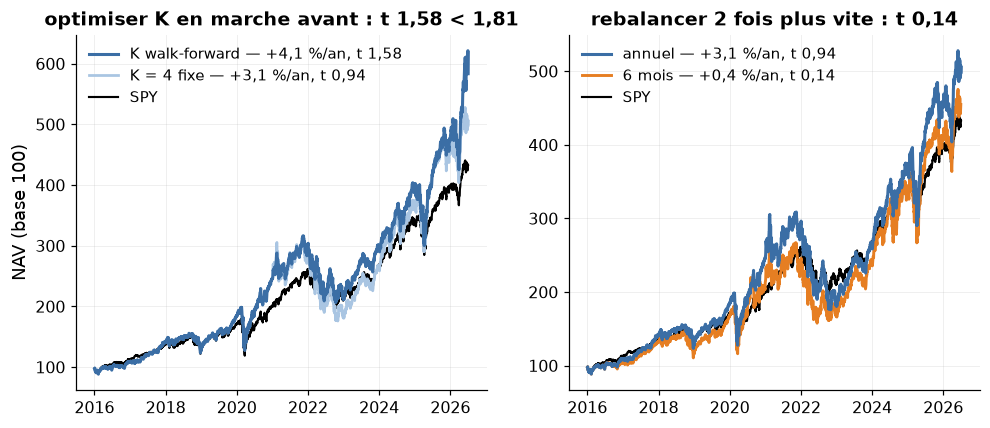
\includegraphics[width=0.66\textwidth]{fig_05b_k_et_cadence.png}\\[1.5mm]
  \badge{helec}{K walk-forward : +4,1 \%/an, t = 1,58 < 1,81}\;
  \badge{warnorange}{6 mois : +0,4 \%/an, t = 0,14}\\[1.2mm]
  {\scriptsize\color{black!60} plus de liberté sur $K$ et la cadence — le $t$ monte un peu, ne passe jamais le seuil}
\end{frame}

% ── B7 · On pousse encore : changer la pondération ──
\begin{frame}{On pousse encore : changer la répartition du capital}
  \begin{columns}[T]
    \begin{column}{0.46\textwidth}
      {\footnotesize au lieu de $1/K$, on pondère par le \textbf{risque} :}\\[2mm]
      {\footnotesize \textbf{inverse-vol} — $w_k \propto 1/\sigma_k$\\[1mm]
       \textbf{ERC} — contributions au risque égales\\[1mm]
       \textbf{GMV} — variance minimale, $\min_{w}\, w^{\top}\Sigma w$}\\[2.5mm]
      {\scriptsize\color{black!60} + on stabilise $\Sigma$ par shrinkage (Ledoit-Wolf) — détail en annexe}
    \end{column}
    \begin{column}{0.52\textwidth}\centering
      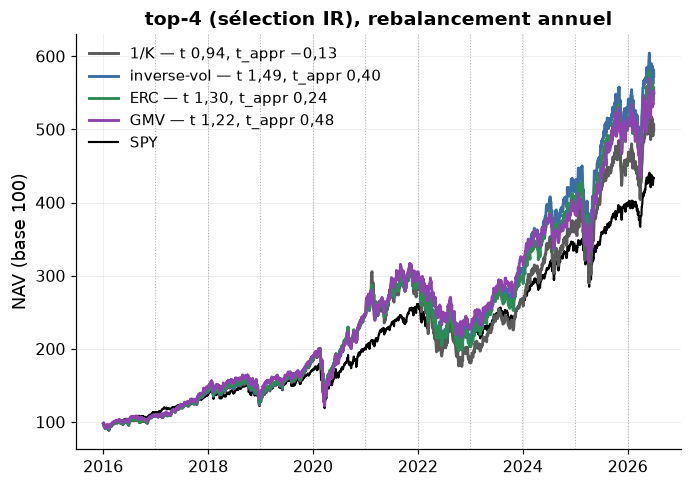
\includegraphics[width=\linewidth]{fig_05b_ponderations.png}\\[1mm]
      \badgel{hocr}{inverse-vol : t 0,94 → 1,49}\;
      \badge{alertred}{GMV : sur-ajuste, −4,5 \%/an}
    \end{column}
  \end{columns}
  \vspace{1.5mm}
  \centering
  {\scriptsize\color{black!60} \textbf{max $t_{\text{appr}} = +0{,}48$} sur toutes les pondérations —
   aucune ne fait apparaître d'$\alpha$}
\end{frame}

% ═════════════ CHAPITRE C — STRATÉGIE 2 ═════════════
\chapdivider{Chapitre C · Stratégie 2}{Changer de règle : le Sharpe}{ni $K$, ni la cadence, ni les poids n'ont passé le seuil — on change la règle de sélection}

% ── C1 · Le Sharpe brut ──
\begin{frame}{Nouvelle règle : classer au Sharpe brut, sans test de significativité}
  \centering
  {\footnotesize $\mathrm{Sharpe}=\dfrac{\overline{r_P}}{\sigma(r_P)}\sqrt{252}$ ;\quad
   éligible v2 $\iff n_{\text{jours}}\ge 126$ \textbf{et} $\mathrm{Sharpe}>0{,}4$ — \textbf{plus aucun test t}}\\[1.5mm]
  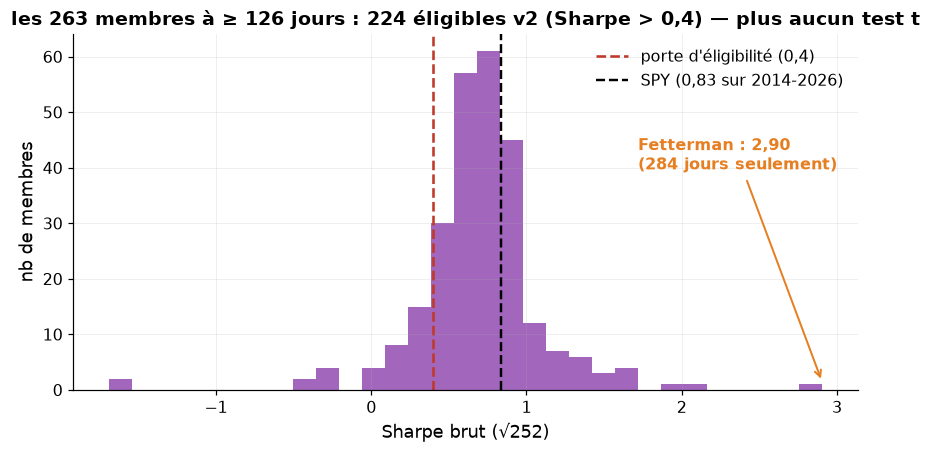
\includegraphics[height=0.52\textheight]{fig_05b_hist_sharpe.png}\\[1.5mm]
  {\footnotesize \textbf{224} éligibles (vs 223 en stratégie 1 — presque les mêmes) ;
   \textbf{même moteur} de copie en parts, seule la règle de classement change}\\[0.4mm]
  {\scriptsize\color{black!60} au prix d'admettre des historiques courts en tête (Fetterman 284 j, Sewell 4 trades)}
\end{frame}

% ── C2 · Balayage K ──
\begin{frame}{Même résultat : le $t$ plafonne à 1,22, loin du seuil}
  \centering
  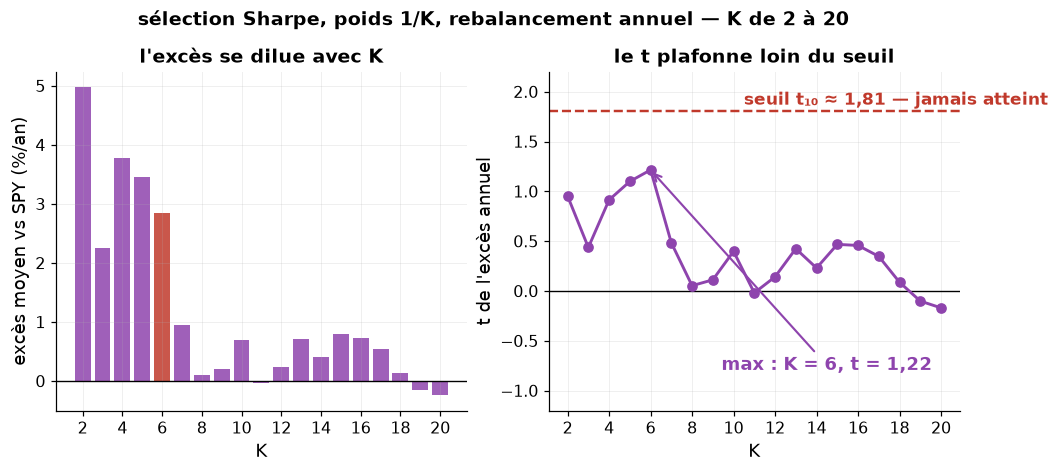
\includegraphics[width=0.62\textwidth]{fig_05b_balayage_k.png}\\[2mm]
  {\footnotesize testé sur \textbf{5 pondérations × $K$ de 2 à 20 × 2 cadences} : le meilleur cas est $K=6$,
   \textbf{$t=1{,}22$} ($<1{,}81$) ; l'excès se dilue quand $K$ grandit}\\[0.6mm]
  {\scriptsize\color{black!60} Sharpe 0,93 vs SPY 0,87 — le couple rendement/risque ne bouge pas ;
   pas mieux que la stratégie 1}
\end{frame}

% ═════════════ CHAPITRE D — VERDICT ═════════════
% ── D1 · Verdict ──
\begin{frame}{Verdict : un $\beta$ de style $\approx$ 1,2 — et zéro alpha, sous toutes les coutures}
  \centering
  \resizebox{0.97\textwidth}{!}{%
  \begin{tikzpicture}[node distance=4.5mm]
    \node[bande=helec, text width=2.9cm] (q1) {\textbf{QUI}\\[0.5mm]IR · appraisal · Sharpe};
    \node[bande=helec, text width=2.9cm, right=of q1] (q2) {\textbf{COMBIEN}\\[0.5mm]$K\in[2,20]$, fixe\\ou walk-forward};
    \node[bande=helec, text width=2.9cm, right=of q2] (q3) {\textbf{QUAND}\\[0.5mm]annuel · 6 mois};
    \node[bande=helec, text width=2.9cm, right=of q3] (q4) {\textbf{COMMENT}\\[0.5mm]5 pondérations ×\\4 estimateurs $\Sigma$};
    \node[bande=alertred, text width=2.4cm, right=of q4] (q5) {\textbf{même\\verdict}};
    \draw[arr] (q1) -- (q2); \draw[arr] (q2) -- (q3);
    \draw[arr] (q3) -- (q4); \draw[arr] (q4) -- (q5);
  \end{tikzpicture}}\\[4mm]
  \tuile{alertred}{1,58}{max $t$, stratégie 1\\(seuil 1,81)}\hfill
  \tuile{alertred}{1,22}{max $t$, stratégie 2\\(seuil 1,81)}\hfill
  \tuile{alertred}{+0,99}{max $t_{\text{appr}}$, tout compris\\(seuil 1,645)}\hfill
  \tuile{warnorange}{$\beta$ ≈ 1,20}{l'excès brut n'était\\que du style}\\[2.5mm]
  {\footnotesize ce n'est pas un réglage manqué : ni \emph{qui}, ni \emph{combien},
   ni \emph{quand}, ni \emph{comment} — rien n'apporte d'$\alpha$}
\end{frame}

% ── D2 · La suite ──
\begin{frame}{Un résultat négatif propre — et trois portes encore ouvertes}
  \begin{columns}[T]
    \begin{column}{0.32\textwidth}
      \carte{helec}{Le signal événementiel}{réagir au moment de la \textbf{divulgation}
       des PTR (fenêtres courtes autour du dépôt), plutôt que détenir en continu}
    \end{column}
    \begin{column}{0.32\textwidth}
      \carte{selec}{Le protocole pré-enregistré}{hypothèses, grille de tests et jalons
       \textbf{gelés avant} de regarder les données — plus de balayage a posteriori}
    \end{column}
    \begin{column}{0.32\textwidth}
      \carte{okgreen}{L'out-of-sample}{\textbf{geler} les règles, juger sur les données
       neuves que le pipeline S1-S2 continue de capter}
    \end{column}
  \end{columns}
  \vspace{5mm}
  \centering
  \badge{grisC}{et POURQUOI le classement ne pouvait pas marcher : l'autopsie (Partie III) — au prochain épisode}\\[3mm]
  {\footnotesize savoir que ça ne marche pas — \textbf{et pouvoir le prouver} — est déjà un actif de recherche}
\end{frame}

% ═════════════ ANNEXE — PARTIE II : compléments techniques ═════════════
\chapdivider{Annexe · Partie II}{Sous le capot}{le détail technique : shrinkage de $\Sigma$, contre-preuve membre par membre, moteur en parts}

% ── An3 · Ledoit-Wolf (ex-S3-14) ──
\begin{frame}{Le shrinkage répare l'estimateur de $\Sigma$ — pas la stratégie}
  \centering
  {\footnotesize $\Sigma_{\text{shrink}}=\delta\,F+(1-\delta)\,\Sigma_{\text{emp}}$,\;
   $\delta=\frac{\pi-\rho}{T\gamma}$ borné à $[0,1]$ —
   3 cibles $F$ : diagonale (LW 2004) · single-factor (LW 2001) · corrélation constante (LW 2003)}\\[1mm]
  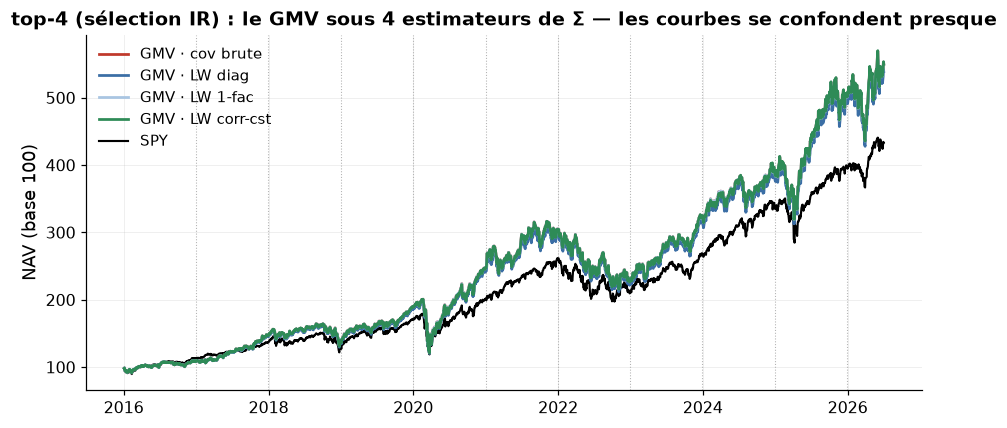
\includegraphics[height=0.40\textheight]{fig_05b_gmv_ledoitwolf.png}\\[1.5mm]
  \tuile{okgreen}{−4,5 → −4,3}{\%/an : l'artefact GMV\\(sél. appr) tempéré}\hfill
  \tuile{okgreen}{−2,76 → −2,46}{le t remonte…\\sans devenir positif}\hfill
  \tuile{helec}{50 → 25}{conditionnement\\de $\Sigma$ (LW diag)}\hfill
  \tuile{grisC}{0,67 → 0,55}{concentration HHI\\du panier GMV}\\[1.5mm]
  {\scriptsize\color{black!60} intensité mesurée $\delta_{\text{LW}} \approx 0{,}05$ —
   verdict invariant à l'estimateur : \textbf{$\beta$ de style $\approx$ 1,20, zéro $\alpha$}}
\end{frame}

% ── An4 · Contre-preuve IR ↔ β (ex-S3-8) ──
\begin{frame}{La contre-preuve point par point : la queue droite de l'IR, c'était du $\beta$}
  \centering
  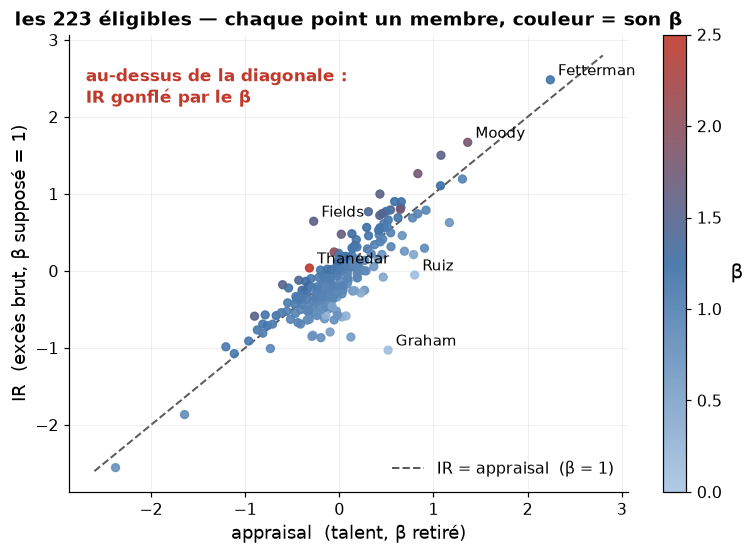
\includegraphics[height=0.63\textheight]{fig_05b_ir_vs_appraisal.png}\\[1mm]
  {\footnotesize au-dessus de la diagonale : classé par l'IR \textbf{grâce à son $\beta$} —
   l'ajustement dégonfle la queue droite}\\[0.8mm]
  {\scriptsize\color{black!60} c'est la version « membre par membre » du 20 → 12 :
   on juge chaque stratégie en excès brut \textbf{et} en $t_{\mathrm{appr}}$}
\end{frame}

% ── An5 · Moteur en parts détaillé (ex-S3-10) ──
\begin{frame}{Le moteur en parts, en détail : compter, redéployer, tenir}
  \centering
  {\footnotesize membre $k$ = un fonds au prix de part $\mathrm{NAV}^k(t)=\prod_{s\le t}(1+r_k(s))$ ;
   on en détient $\mathrm{nbr}^k$ parts ; poids cibles $w_k=1/|S_Y|$ ; capital initial $W = 100$}\\[4mm]
  \resizebox{0.98\textwidth}{!}{%
  \begin{tikzpicture}[node distance=7mm]
    \node[step=grisC, text width=4.4cm] (n1)
      {\textbf{(i) COMPTER} à la coupe $t^R_Y$\\[1.5mm]
       $\displaystyle W=\!\!\sum_{k\in S_{Y-1}}\!\!\mathrm{nbr}^k_{Y-1}\,\mathrm{NAV}^k(t^R_Y)$};
    \node[step=helec, text width=4.0cm, right=of n1] (n2)
      {\textbf{(ii) REDÉPLOYER} sur la nouvelle sélection $S_Y$\\[1.5mm]
       $\displaystyle \mathrm{nbr}^k_Y=\frac{w_k\,W}{\mathrm{NAV}^k(t^R_Y)}$};
    \node[step=okgreen, text width=5.0cm, right=of n2] (n3)
      {\textbf{(iii) TENIR} (buy-and-hold, parts figées)\\[1.5mm]
       $\displaystyle \mathrm{NAV}(t)=\sum_{k\in S_Y}\mathrm{nbr}^k_Y\,\mathrm{NAV}^k(t)$\\[1mm]
       $\displaystyle r_{\text{strat}}(t)=\frac{\mathrm{NAV}(t)}{\mathrm{NAV}(t{-}1)}-1$};
    \draw[arr] (n1) -- (n2);
    \draw[arr] (n2) -- (n3);
    \draw[arr] (n3.south) .. controls +(0,-1.1) and +(0,-1.1) .. (n1.south)
      node[midway, below, font=\scriptsize\bfseries, gray] {coupe suivante};
  \end{tikzpicture}}\\[4mm]
  \badge{okgreen}{autofinancé — aucun apport, aucun retrait : la NAV est continue}\;
  \badge{warnorange}{entre deux coupes les poids DÉRIVENT (buy-and-hold, pas constant-mix)}
\end{frame}

% ─────── Annexe · les 5 types de rapports « patrimoine », fiche par fiche ───────
% (déplacées ici depuis le corps du deck ; chiffres : docs/ANALYSE_FILING_TYPES_HOUSE.md)

% ── An-O ── (profil mesuré : 3 835 numériques scannés ; census)
\begin{frame}{Annexe — \texttt{O}, le rapport annuel}
  \begin{columns}[c]
    \begin{column}{0.34\textwidth}\centering
      \href{https://disclosures-clerk.house.gov/public_disc/financial-pdfs/2023/10059952.pdf}{\fcolorbox{black!30}{white}{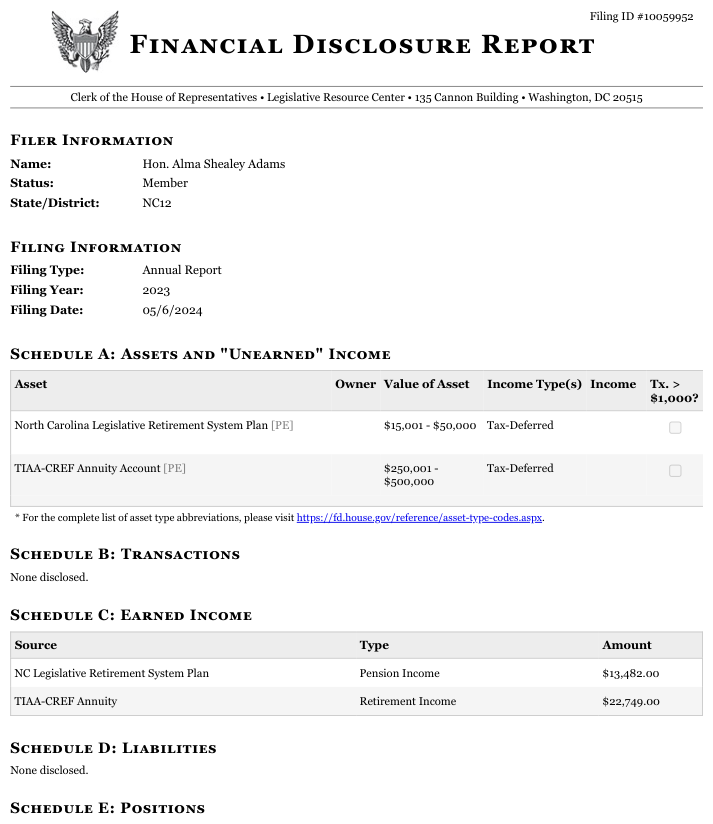
\includegraphics[height=54mm]{slides/ftype_o.png}}}\\[0.5mm]
      {\scriptsize\color{black!60} Alma Adams, 2023 — cliquable}
    \end{column}
    \begin{column}{0.64\textwidth}
      {\footnotesize
      \textbf{Qui, quand} — chaque \textbf{membre en poste}, une fois par an,
      au printemps-été suivant l'année couverte (pics mesurés : mai, puis août
      après extension).\\[1.2mm]
      \textbf{Ce qu'il contient} — 9 sections : actifs \& revenus de placement (A),
      \textbf{transactions de l'année (B)}, salaires (C), dettes (D), postes occupés (E),
      accords (F), cadeaux (G), voyages payés (H), dons reçus (I).\\[1.2mm]
      \textbf{En chiffres} — \textbf{4\,625} dépôts (98 \% de membres) ·
      3\,905 numériques / \textbf{720 scannés} · 5 pages en médiane (jusqu'à 251) ·
      \textbf{31 \%} ont des transactions en Schedule B.}\\[1.5mm]
      \badge{warnorange}{le plus gros gisement hors PTR — divulgué à N+1}
    \end{column}
  \end{columns}
\end{frame}

% ── An-C ── (échantillon 39 numériques : sections A/C/D/E/F/J, 0 % Schedule B)
\begin{frame}{Annexe — \texttt{C}, le rapport de candidat}
  \begin{columns}[c]
    \begin{column}{0.34\textwidth}\centering
      \href{https://disclosures-clerk.house.gov/public_disc/financial-pdfs/2023/10056211.pdf}{\fcolorbox{black!30}{white}{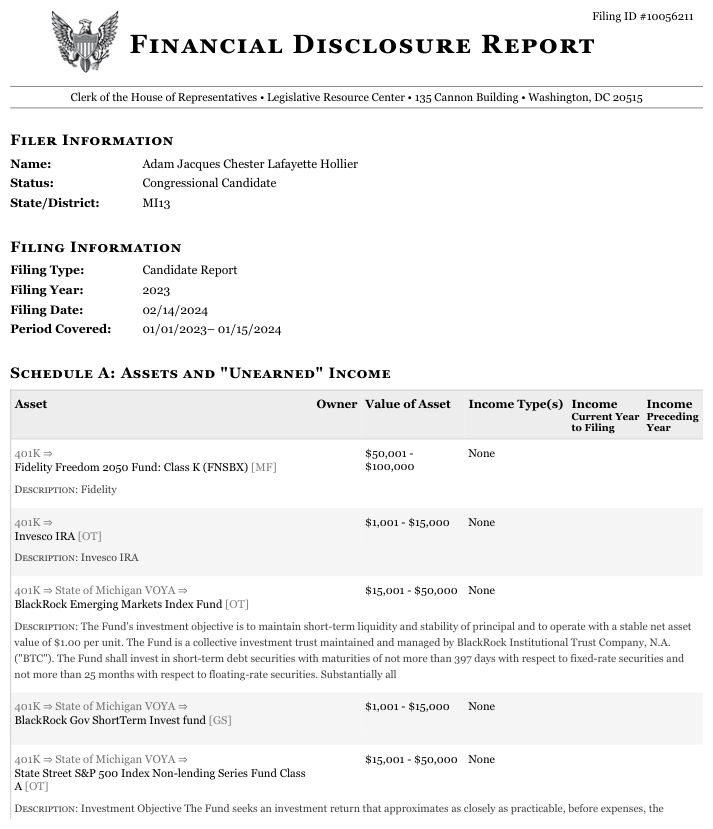
\includegraphics[height=54mm]{slides/ftype_c.png}}}\\[0.5mm]
      {\scriptsize\color{black!60} Adam Hollier, candidat MI13, 2023 — cliquable}
    \end{column}
    \begin{column}{0.64\textwidth}
      {\footnotesize
      \textbf{Qui, quand} — toute personne qui \textbf{se porte candidate} à la
      Chambre (une fois sa campagne au-delà de 5\,000 \$) — avant d'être élue, et
      le plus souvent sans jamais l'être.\\[1.2mm]
      \textbf{Ce qu'il contient} — la photo du patrimoine du candidat :
      actifs (A), salaires (C), dettes (D), postes (E), accords (F),
      compensations >\,5\,000 \$ (J). \textbf{Pas de section transactions} —
      0 sur les 39 échantillonnés.\\[1.2mm]
      \textbf{En chiffres} — \textbf{10\,105} dépôts, le type le plus fréquent de
      l'index · \textbf{77 \% déposés par des candidats jamais élus} ·
      3 pages en médiane.}\\[1.5mm]
      \badge{grisC}{hors périmètre : pas élu, pas de transactions}
    \end{column}
  \end{columns}
\end{frame}

% ── An-H ── (369 numériques : sections A/C/D/E/F/J, 0 % Schedule B)
\begin{frame}{Annexe — \texttt{H}, la déclaration d'entrée}
  \begin{columns}[c]
    \begin{column}{0.34\textwidth}\centering
      \href{https://disclosures-clerk.house.gov/public_disc/financial-pdfs/2023/10062638.pdf}{\fcolorbox{black!30}{white}{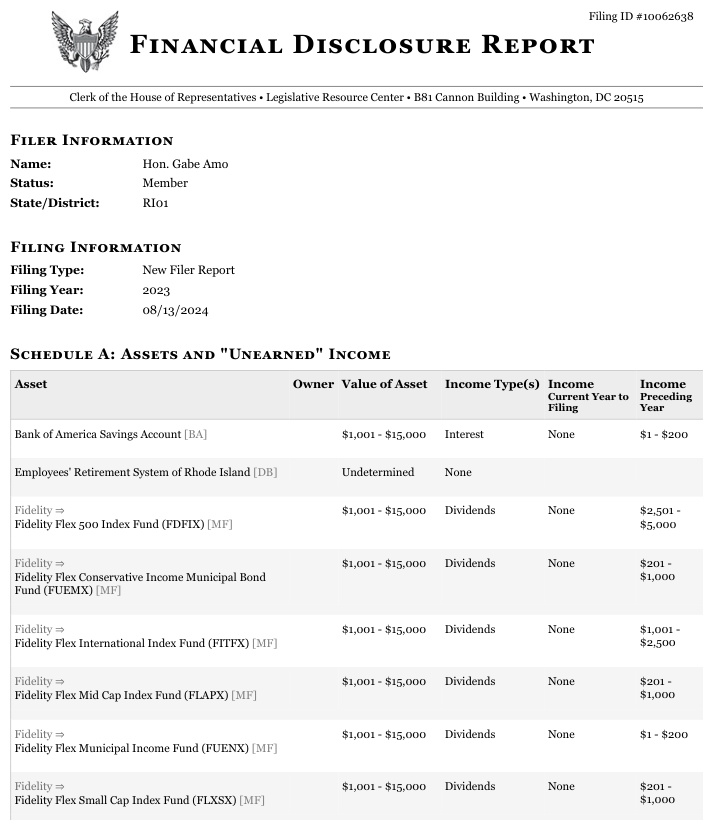
\includegraphics[height=54mm]{slides/ftype_h.png}}}\\[0.5mm]
      {\scriptsize\color{black!60} Gabe Amo, nouveau membre RI01, 2023 — cliquable}
    \end{column}
    \begin{column}{0.64\textwidth}
      {\footnotesize
      \textbf{Qui, quand} — un \textbf{membre qui vient d'entrer en fonction}
      (élection partielle, prise de poste) : sa photo de départ.\\[1.2mm]
      \textbf{Ce qu'il contient} — le même formulaire réduit que le candidat :
      actifs (A), salaires (C), dettes (D), postes (E), accords (F),
      compensations (J). \textbf{Pas de section transactions} —
      0 sur les 369 numériques analysés.\\[1.2mm]
      \textbf{En chiffres} — \textbf{395} dépôts (97 \% membres) ·
      quasi tout numérique (383) · 4 pages en médiane.}\\[1.5mm]
      \badge{grisC}{une photo d'entrée : rien à extraire pour le signal}
    \end{column}
  \end{columns}
\end{frame}

% ── An-T ── (287 numériques : ABCDEFGHI, 28 % Schedule B ; dépôt janv-févr)
\begin{frame}{Annexe — \texttt{T}, la déclaration de sortie}
  \begin{columns}[c]
    \begin{column}{0.34\textwidth}\centering
      \href{https://disclosures-clerk.house.gov/public_disc/financial-pdfs/2023/10050798.pdf}{\fcolorbox{black!30}{white}{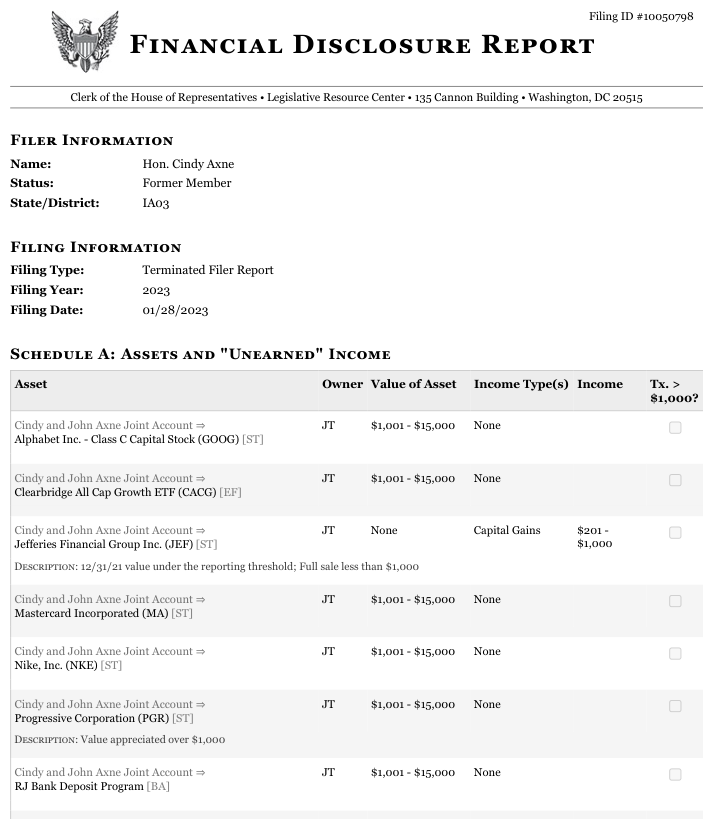
\includegraphics[height=54mm]{slides/ftype_t.png}}}\\[0.5mm]
      {\scriptsize\color{black!60} Cindy Axne, départ de la Chambre, 2023 — cliquable}
    \end{column}
    \begin{column}{0.64\textwidth}
      {\footnotesize
      \textbf{Qui, quand} — un membre qui \textbf{quitte la Chambre} (fin de mandat,
      démission) — déposé surtout en janvier-février suivant le départ (mesuré).\\[1.2mm]
      \textbf{Ce qu'il contient} — le formulaire complet du rapport annuel
      (9 sections, \textbf{dont les transactions (B)}) sur l'année partielle
      jusqu'au départ. \textbf{28 \%} en contiennent.\\[1.2mm]
      \textbf{En chiffres} — \textbf{392} dépôts (99 \% membres) ·
      292 numériques / 100 scannés · 5 pages en médiane.\\[1.2mm]
      \textbf{Exemple réel} — la sortie d'Eric Cantor (2014) contient des achats
      d'ETF jamais déposés en PTR — ils font partie des 173 trades « annuel-seul ».}\\[1.5mm]
      \badge{warnorange}{petite source de trades manqués — surtout 2014-2016}
    \end{column}
  \end{columns}
\end{frame}

% ── An-A ── (1 285 numériques : sections du doc corrigé, 26 % Schedule B)
\begin{frame}{Annexe — \texttt{A}, l'amendement}
  \begin{columns}[c]
    \begin{column}{0.34\textwidth}\centering
      \href{https://disclosures-clerk.house.gov/public_disc/financial-pdfs/2023/10062190.pdf}{\fcolorbox{black!30}{white}{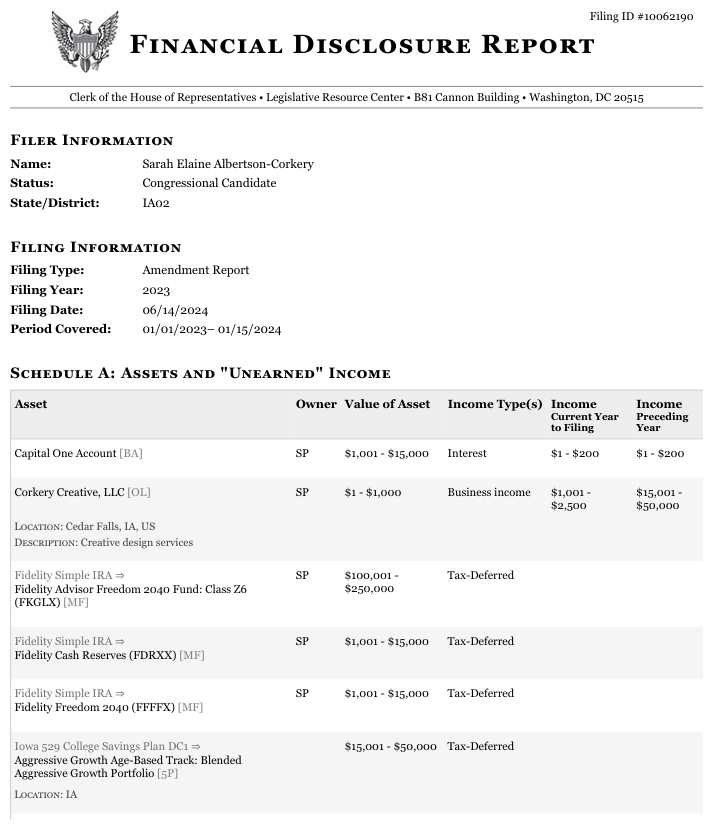
\includegraphics[height=54mm]{slides/ftype_a.png}}}\\[0.5mm]
      {\scriptsize\color{black!60} Sarah Albertson-Corkery, 2023 — cliquable}
    \end{column}
    \begin{column}{0.64\textwidth}
      {\footnotesize
      \textbf{Qui, quand} — n'importe quel déposant qui \textbf{corrige un dépôt
      antérieur} (annuel, candidat, sortie…) — le document corrigé est re-déposé
      en entier.\\[1.2mm]
      \textbf{Ce qu'il contient} — les sections \textbf{du document qu'il corrige} :
      un amendement d'annuel a une Schedule B, un amendement de candidat n'en a pas
      (mesuré : 26 \% avec transactions).\\[1.2mm]
      \textbf{En chiffres} — \textbf{2\,298} dépôts (72 \% membres,
      le reste candidats) · 5 pages en médiane.\\[1.2mm]
      \textbf{Piège mesuré} — l'amendement \textbf{répète} les trades de l'annuel
      qu'il corrige (ex. Pelosi 2014 : le même trade apparaît 3 fois O+A+A) —
      notre mesure les dédoublonne.}\\[1.5mm]
      \badge{grisC}{rien de neuf en soi : suit le sort du document corrigé}
    \end{column}
  \end{columns}
\end{frame}

\end{document}
